\documentclass[aspectratio=169]{beamer}
\usetheme{metropolis}
\usepackage{booktabs}
\title{AI: The Big Picture}
\subtitle{A dive into the past, present and future of frontier AI development}
\author{Kai Zuberbühler}
\date{\today}
\usepackage[backend=biber,
    style=apa]{biblatex}
\usepackage{cleveref}
\usepackage{textcomp}
\usepackage{mfirstuc}
\addbibresource{references.bib}

% Fixes
\DeclareFieldFormat{title}{\capitalisewords{#1}}
\setbeamertemplate{bibliography item}{}
\setlength{\bibhang}{0em}
\setlength{\itemindent}{-\bibhang}

\begin{document}
    \frame{\titlepage}
    \begin{frame}{Table of Contents}
        \setbeamertemplate{section in toc}[sections numbered]
        \tableofcontents[hideallsubsections]
    \end{frame}


    \section{Scaling}
    \begin{frame}
        \frametitle{Main Factors for Training Better AI Models}
        \begin{itemize}
            \item Size (Parameter Count)
            \begin{itemize}
                \item Increase the size of the model which requires \alert{more compute}
                \item Drawback: During inference, the model also requires \alert{more compute}
                \item Has not really grown anymore in the past years (GPT-4.5 is a notable exception).
            \end{itemize}
            \item Quality of Data
            \begin{itemize}
                \item One approach: Filter and augment data using AI which requires \alert{more compute}
            \end{itemize}
            \item Quantity of Data
            \begin{itemize}
                \item Increase the size of the training dataset which requires \alert{more compute}
                \item Another approach: Generate new data using AI which requires \alert{more compute}
            \end{itemize}
            \item Architecture
            \begin{itemize}
                \item Increase research which requires more researchers and \alert{more compute}
                \item Roughly equivalent to tripling compute per year~\parencite{ho_algorithmic_2024}
            \end{itemize}
        \end{itemize}
    \end{frame}
    \begin{frame}{Scaling Law Formulas}
        \begin{figure}
            \[
                \text{Performance} = \log(\text{Model Size} \cdot \text{Data Quantity} \cdot \text{Data Quality} \cdot \text{Architecture Efficiency})
            \]
            \caption{Oversimplified scaling law for language models}
        \end{figure}
        \begin{figure}
            \[
                \hat{L}(N, D) \triangleq E + \frac{A}{N^\alpha} + \frac{B}{D^\beta}
            \]
            \caption{Scaling law for language models where L is the loss of the model, N is the number of model parameters and D is the number of training tokens~\parencite{hoffmann_training_2022}}
        \end{figure}
    \end{frame}
    \begin{frame}{Predicting Loss with Scaling Laws Is Easy ...}
        \begin{figure}
            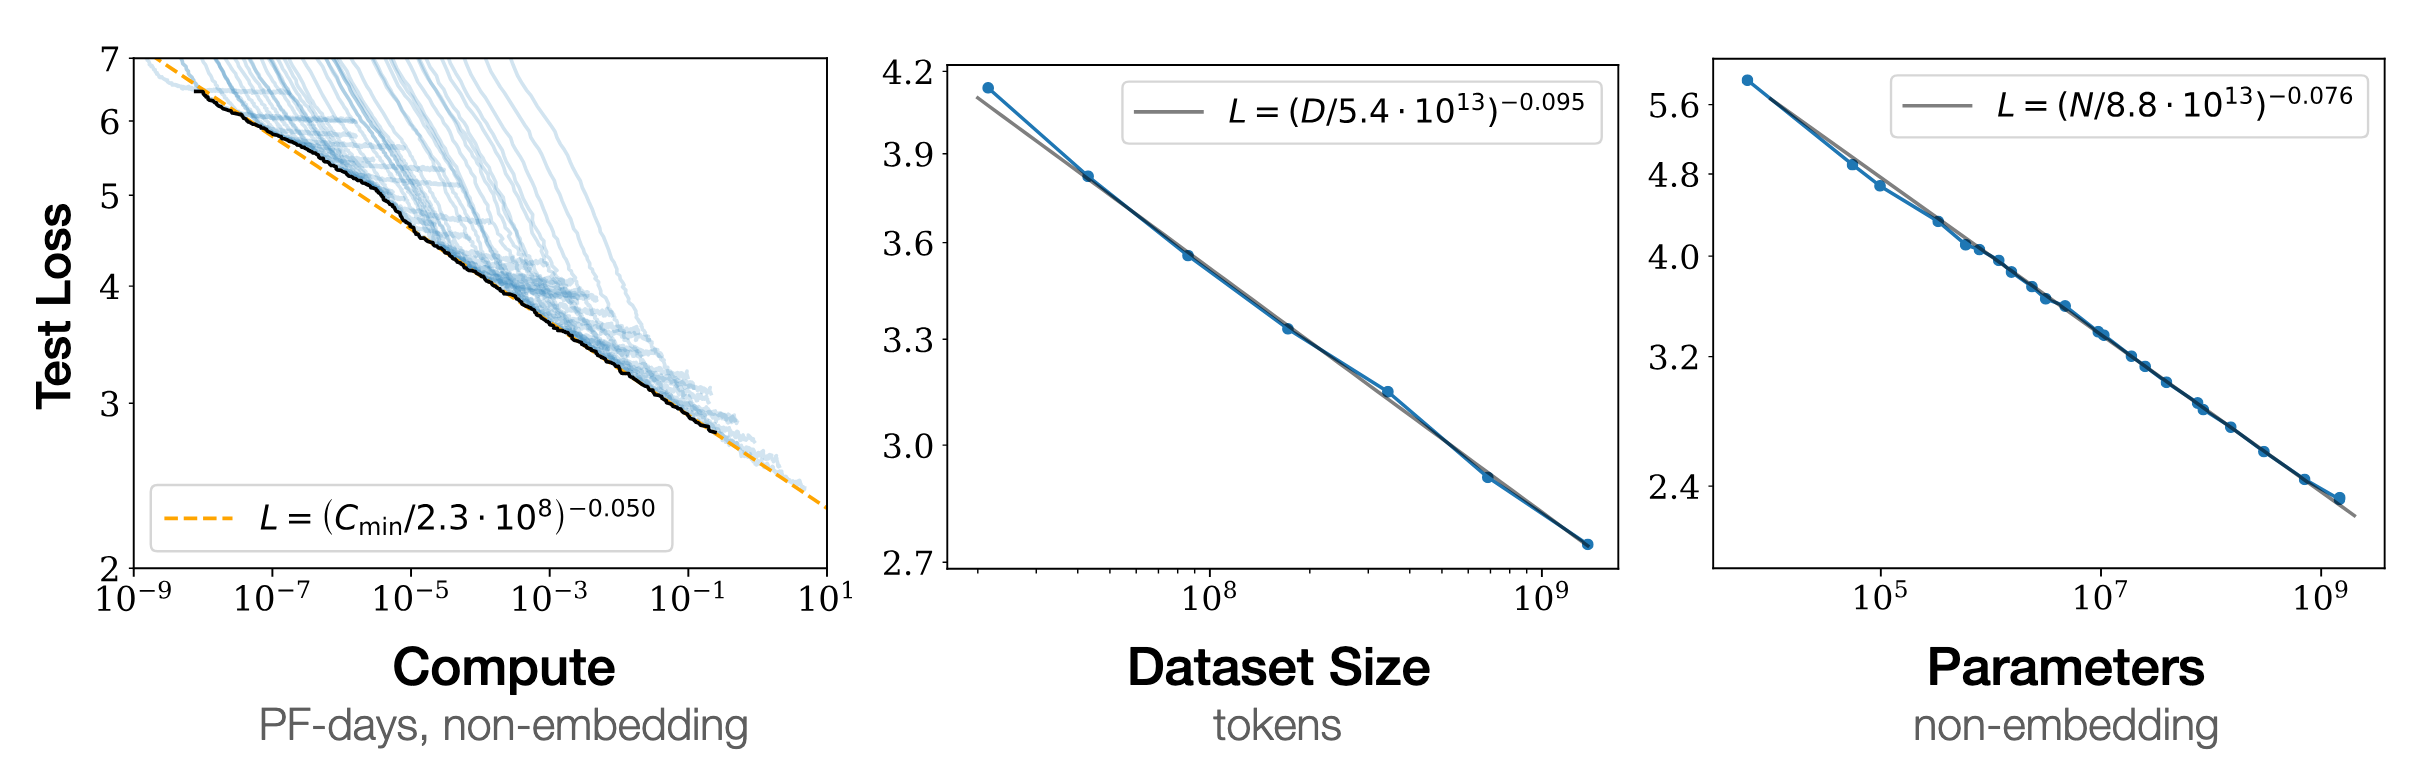
\includegraphics[width=1\textwidth]{images/kaplan-et-al-2020-scaling}
            \caption{Observed log-linear language model performance improvements with increasing compute, dataset size and parameters~\parencite{kaplan_scaling_2020}}
        \end{figure}
    \end{frame}
    \begin{frame}{... But Predicting Benchmark Performance Is Harder}
        \begin{figure}
            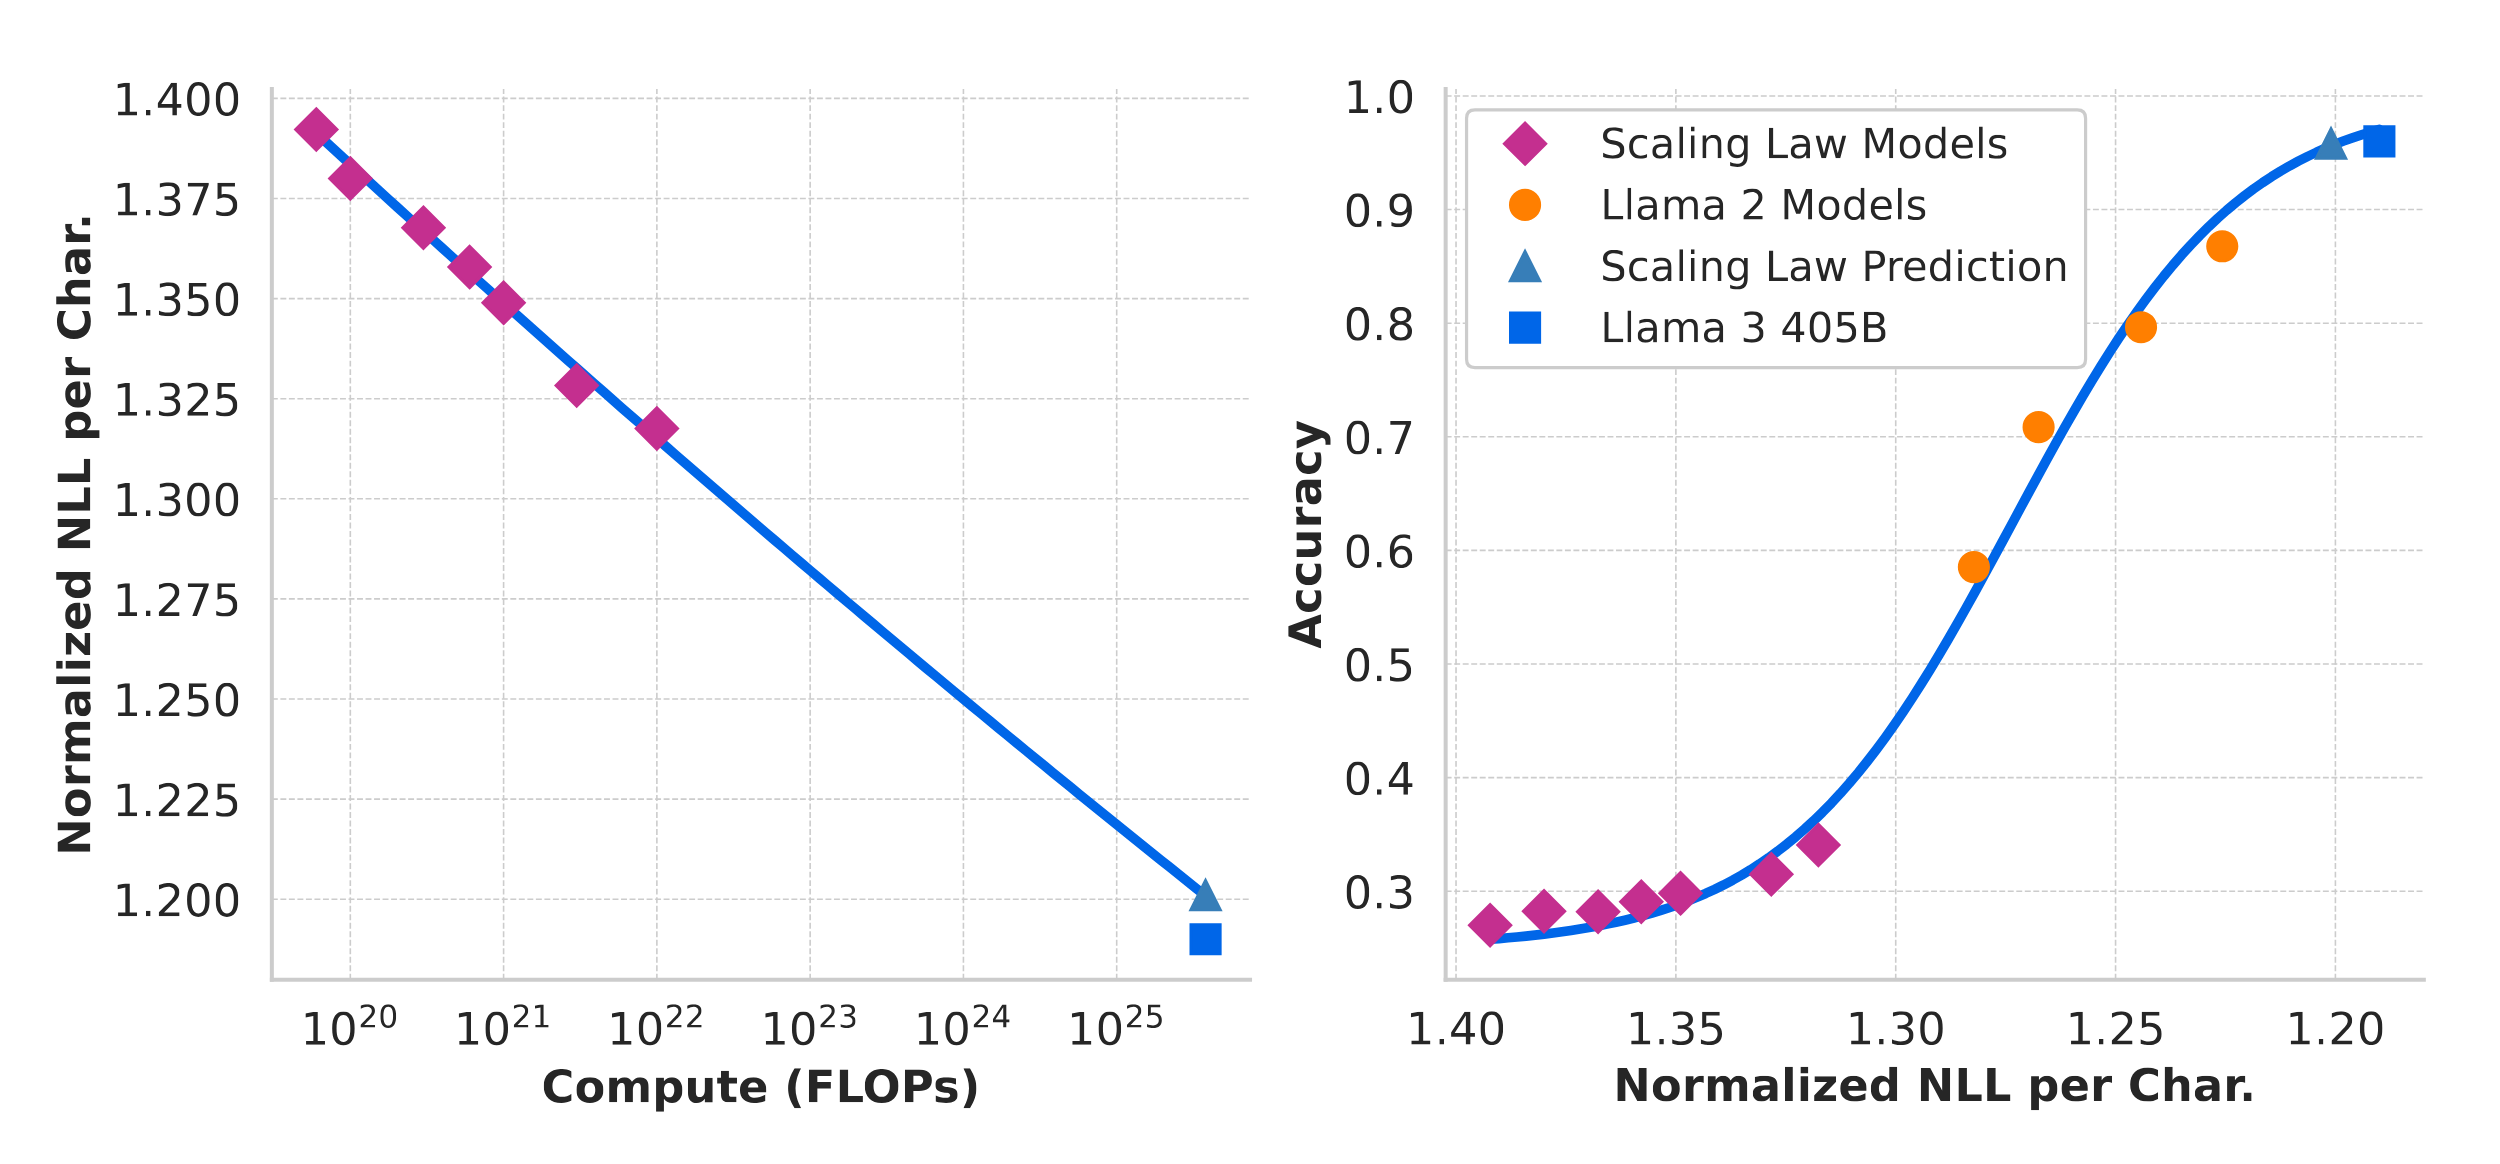
\includegraphics[height=0.35\textwidth]{images/llama-3-scaling-law-prediction}
            \caption{Predicted and observed performance on the ARC Challenge benchmark for the Llama 3 models. At some point, the performance on the benchmark starts to increase faster than an extrapolation would have suggested.~\parencite{grattafiori_llama_2024}}
        \end{figure}
    \end{frame}
    \begin{frame}
        \frametitle{Training Compute of Frontier AI Models Grows by About 4-5x Per Year}
        \begin{figure}
            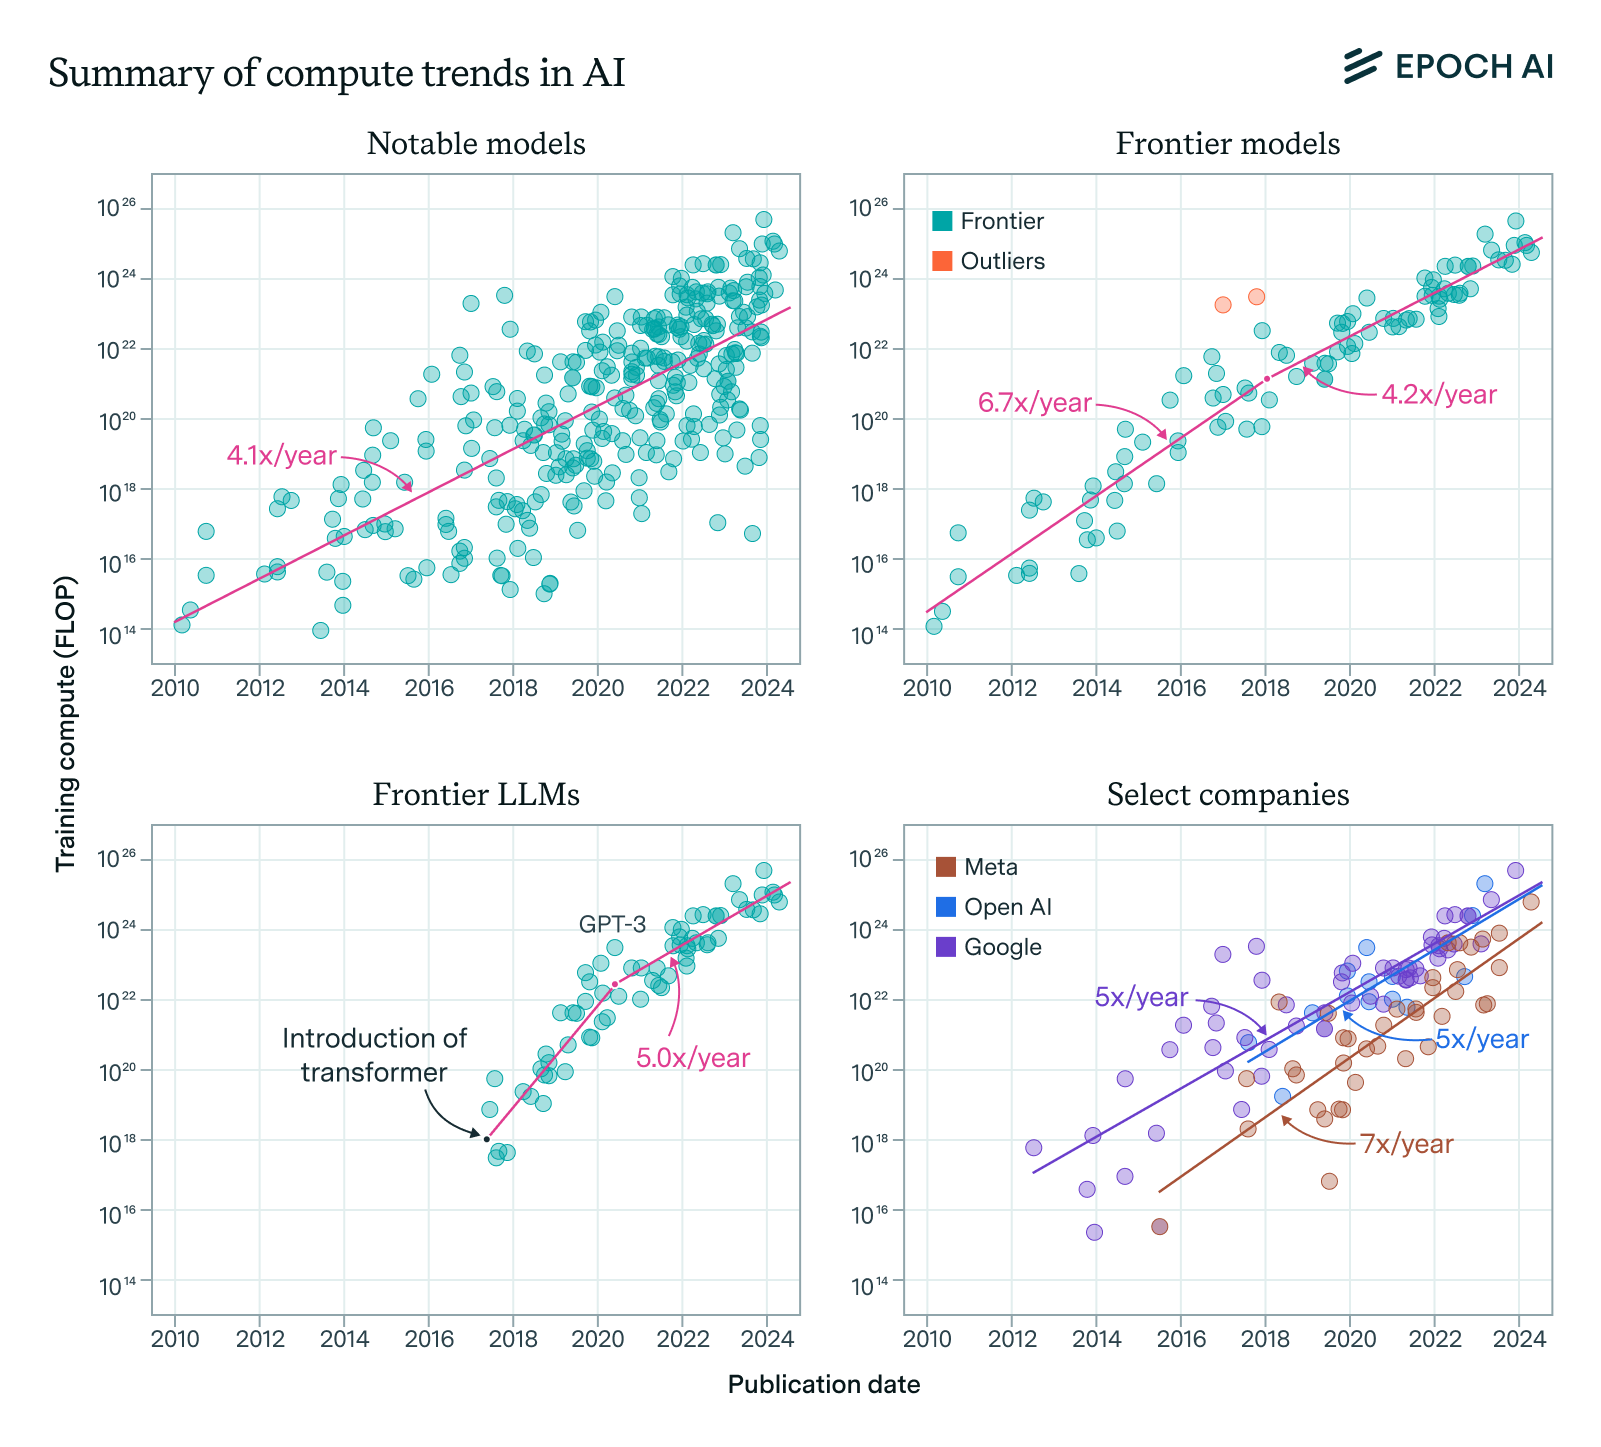
\includegraphics[height=0.45\textwidth]{images/summary_figure}
            \caption{Summary of compute trends in AI~\parencite{epoch2024trainingcomputeoffrontieraimodelsgrowsby45xperyear}}
        \end{figure}
    \end{frame}
    \begin{frame}
        \frametitle{Can AI Scaling Continue Through 2030?}
        \begin{itemize}
            \item Epoch AI, a research institute, released a lengthy report in August 2024 about whether scaling AI at the current trajectory can continue through 2030~\parencite{epoch2024canaiscalingcontinuethrough2030}
            \item They identify and research \alert{electric power}, \alert{chip manufacturing}, \alert{data} and \alert{latency} as key constraints.
            \item Much information is this presentation comes from this report or other reports by Epoch AI\@.
            \item Due to the emergence of reasoning models and news on the data center build-outs, the report is already pretty outdated.
        \end{itemize}
    \end{frame}
    
    \begin{frame}
        \frametitle{Scaling: In a Nutshell}
        \begin{itemize}
            \item The training compute of frontier AI models continues to grow by 4-5x per year, following a log-linear scaling trend that has persisted for over a decade.
            \item Improving AI performance requires more compute through scaling model size, data quantity, data quality, or architecture efficiency.
            \item Scaling laws reliably predict model loss, but benchmark performance is significantly less predictable.
            \item Epoch AI's analysis identifies electric power, chip manufacturing, data availability, and latency as key constraints that must be overcome to maintain the current scaling trajectory through 2030.
        \end{itemize}
    \end{frame}


    \section{Data and Architecture}
    \begin{frame}
        \frametitle{Training Phases of Language Models}
        \begin{itemize}
            \item Pre-Training~\parencite{radford_language_2019}
            \begin{itemize}
                \item Model learns to predict the next token based on the given context
                \item Dataset of text and other modalities mostly from publicly available data
                \item Can be seen as ``System 1'' (fast thinking)
            \end{itemize}
            \item Instruction-Tuning / RLHF~\parencite{wei_finetuned_2021, ouyang_training_2022}
            \begin{itemize}
                \item Model learns to converse and follow instructions in a specific way
                \item Dataset with user-assistant conversations or human preference data
                \item Key to making language models usable for everyday people (see ChatGPT)
            \end{itemize}
            \item Reinforcement Learning to Scale Chain-of-Thought Reasoning~\parencite{openai_o1_system_card_2024}
            \begin{itemize}
                \item Model learns to use chain-of-thought to ``think'' longer to solve problems
                \item Dataset with problems and corresponding solutions through which the model develops successful chain-of-thought reasoning strategies on its own
                \item Can be seen as ``System 2'' (slow thinking)
                \item First introduced in September 2024 by OpenAI and has become the main focus of AI labs in the past few months
            \end{itemize}
        \end{itemize}
    \end{frame}
    \begin{frame}
        \frametitle{Non-Reasoning Models Significantly Under-Perform Humans In Key Areas}
        Key domains with benchmark examples:
        \begin{itemize}
            \item Reasoning
            \begin{itemize}
                \item ARC-AGI-Pub~\parencite{chollet_o3_2024}
                \begin{itemize}
                    \item Semi-Private Eval: 14\% (Claude 3.5 Sonnet) vs.\ 77\% (MTurkers)
                    \item Public Eval: 21\% (Claude 3.5 Sonnet) vs.\ 64\% (Humans)~\parencite{legris2024harcrobustestimatehuman}
                \end{itemize}
            \end{itemize}
            \item Planning
            \begin{itemize}
                \item PlanBench~\parencite{valmeekam2024llmscantplanlrms}
                \begin{itemize}
                    \item Mystery Blocksworld (0-shot): 1\% (Llama 3.1 405B)
                \end{itemize}
            \end{itemize}
            \item Autonomy
            \begin{itemize}
                \item OSWorld~\parencite{OSWorld}
                \begin{itemize}
                    \item 22\% (Claude 3.5 Sonnet, with Screenshots) vs.\ 72\% (Humans)
                \end{itemize}
                \item GAIA~\parencite{mialon2023gaia}
                \begin{itemize}
                    \item 65\% (h2oGPTe Agent using Claude 3.5 Sonnet) vs.\ 92\% (Humans)
                \end{itemize}
            \end{itemize}
        \end{itemize}
    \end{frame}
    \begin{frame}
        \frametitle{Will We Run Out Of Human-Made Data for Pre-Training?}
        \begin{itemize}
            \item The indexed web is estimated to contain roughly 500 trillion tokens of human-generated text and will grow by approximately 50\% by 2030
            \begin{itemize}
                \item About 30 times larger than the largest datasets currently used (about 15 trillion tokens).
                With the current trajectory, we would hit the ``data wall'' in about five years.
            \end{itemize}
            \item It's possible to train several times over the same data (multiple epochs)
            \item Inclusion of other modalities (like images, video and audio), the ``deep web'' (that includes many social media platforms) and private data can further expand the effective data pool
            \begin{itemize}
                \item Converting multimodal content into text-equivalent tokens could roughly triple the available dataset size
            \end{itemize}
            \item The remaining data is likely of lower quality than the data already used
            \item The median projection from Epoch AI is that it's possible to train models with 80,000x the compute of GPT-4 without significant diminishing returns.
        \end{itemize}
    \end{frame}
    \begin{frame}
        \frametitle{Can We Just Generate More Data?}
        \begin{itemize}
            \item Using AI to generate training data is increasingly used, particularly for model distillation in post-training, but still unproven at large scale for pre-training data
            \item This brings the risk of producing low-quality data, e.g. with hallucinations or a lack of diversity, potentially resulting in ``model collapse''~\parencite{shumailov2024curserecursiontraininggenerated}
            \item Scaling inference-time compute is a possible way to increase model performance when generating data~\parencite{epoch2023tradingoffcomputeintrainingandinference}, especially now with reasoning models
            \item Using AI-driven verifiers (and non-AI verifiers, e.g. code compilers) to filter generated data by assessed quality is a promising approach given that verification is easier than generation~\parencite{feng2024modelcollapsescalingsynthesized}
            \item Any large-scale application will likely use a sophisticated synthetic data generation pipeline and focus on generating new data out of existing data~\parencite{hao2025magamassivegenreaudiencereformulation}
            \item It's unclear how cost-efficient high-quality synthetic data is
        \end{itemize}
    \end{frame}
    \begin{frame}
        \frametitle{The Costs of LLMs Are Plummeting}
        \begin{itemize}
            \item The cost of an AI model with GPT-4-level quality has dropped by around 75x between Q1 and Q4 2024.~\parencite{artificial_analysis_2024}
            \item This drop is due to a variety of factors including training on more and higher quality data, post-training techniques, distillation, architectural improvements (e.g. increased sparsity through mixture-of-experts), software improvements and potentially price dumping.
            \item An analysis of open-weight models shows that the ``capability density'' of LLMs (based on the total parameter count of models and their results on widely used benchmarks) is currently growing exponentially, doubling approximately every three months.~\parencite{xiao2024densinglawllms}
        \end{itemize}
    \end{frame}
    \begin{frame}
        \frametitle{What are ``Reasoning Models'' Exactly?}
        \begin{itemize}
            \item The model ``thinks'' using long chain-of-thought before giving a final answer.
            \item Reinforcement learning (RL) is used on an existing instruction-tuned language model to scale and improve this chain-of-thought ``thinking''.
            \item Each answer is graded by a reward function to steer the model towards longer and more efficient reasoning.
            The reward function could e.g. be an AI model comparing the answer to a sample solution or unit tests for code.~\parencite{kimiteam2025kimik15scalingreinforcement}
            \item Such problem-answer pairs might come from a specialized dataset or be extracted from the web using AI.~\parencite{yeo2025demystifyinglongchainofthoughtreasoning}
            \item Through this training, the model discovers and learns better and longer reasoning chains that result in better answers.
            \item Small-scale domain-specific experiments show that even models as small as 1.5B parameters can develop long chain-of-thought abilities, even on consumer GPUs.~\parencite{tinyzero2025, unsloth_train_2025}
        \end{itemize}
    \end{frame}
    \begin{frame}
        \begin{figure}
            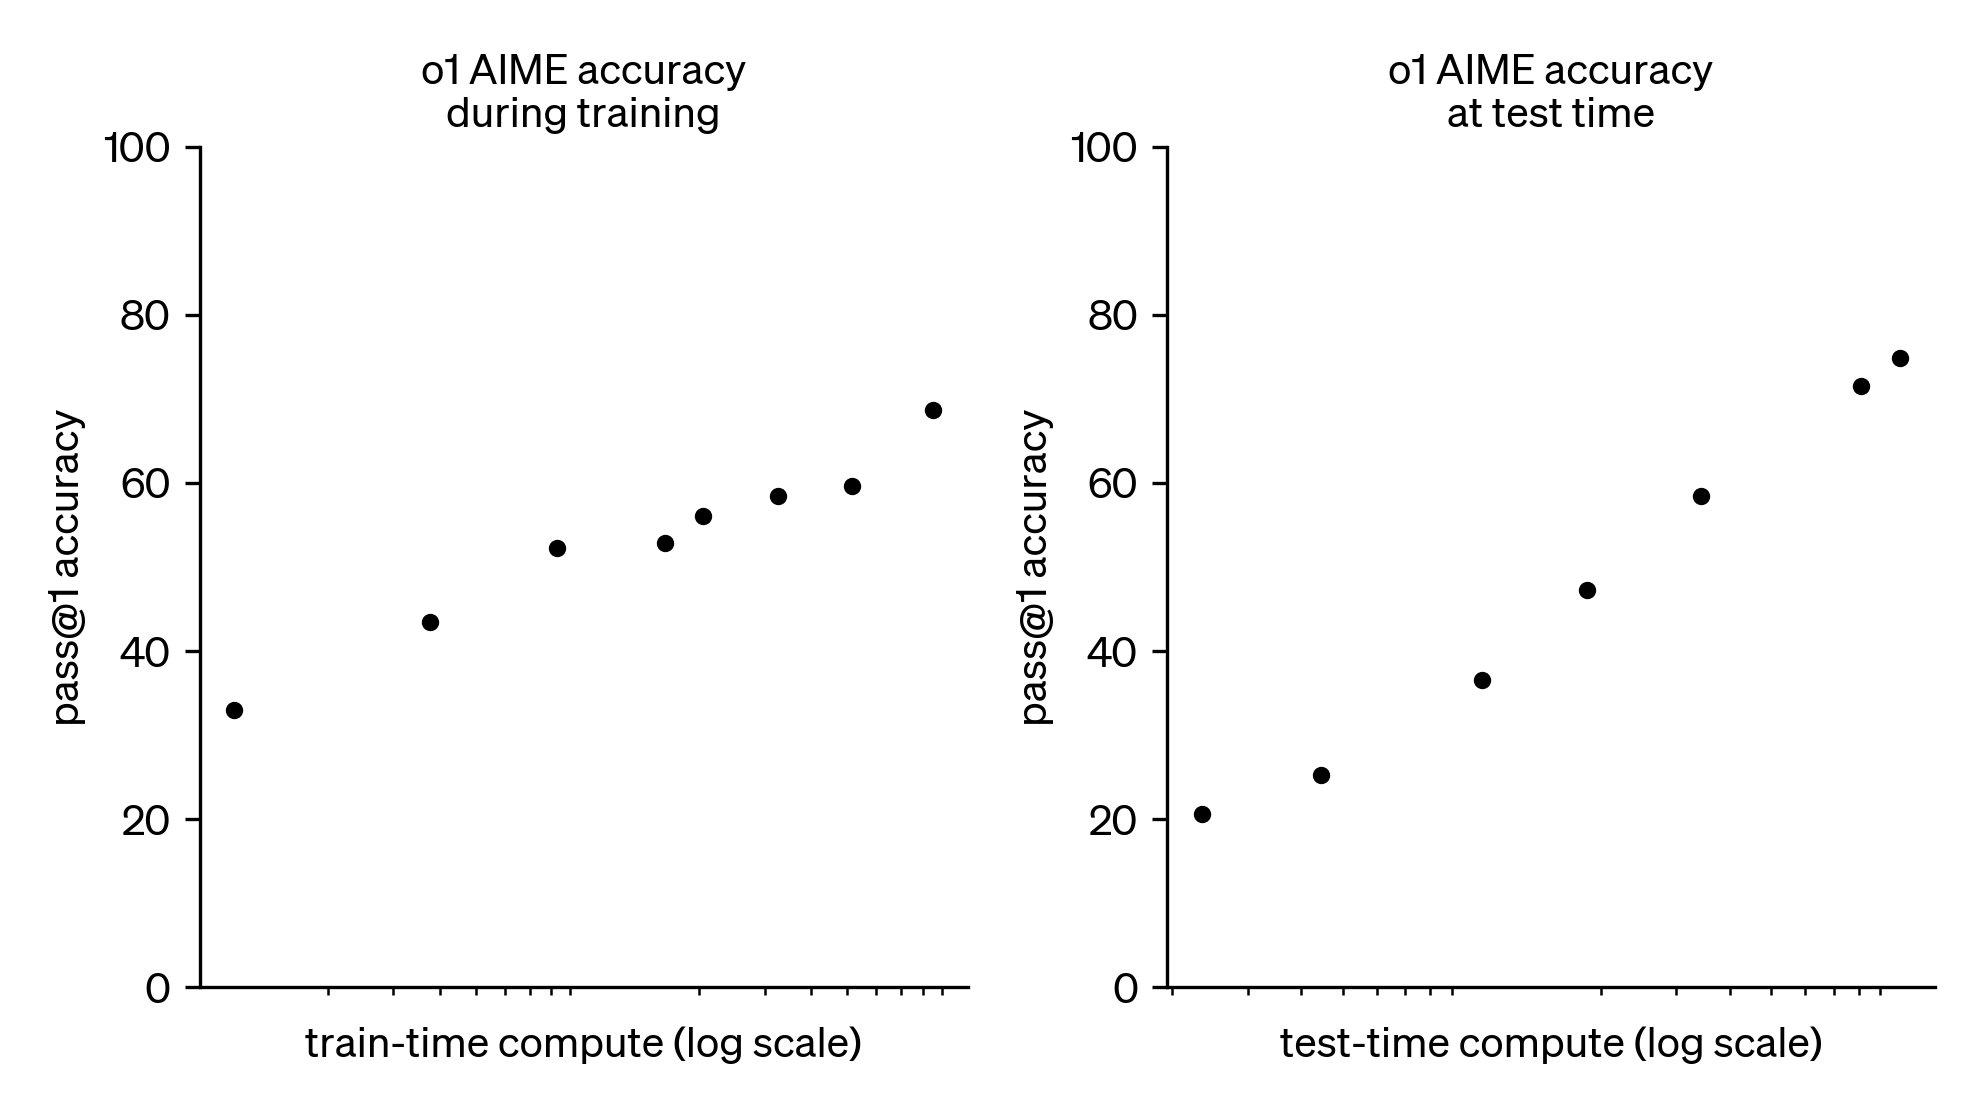
\includegraphics[height=0.45\textwidth]{images/o1-scaling-laws}
            \caption{Reasoning models introduce two new compute scaling paradigms: Scaling chain-of-thought reasoning with reinforcement learning during post-training and scaling the length of the chain-of-thought during inference.~\parencite{openai_learning_to_reason_with_llms_2024}}
        \end{figure}
    \end{frame}
    \begin{frame}
        \frametitle{Benefits of Reasoning Models}
        \begin{itemize}
            \item Reasoning models outperform non-reasoning models in many tasks, most notably and significantly in reasoning, mathematics and coding.
            \begin{itemize}
                \item Top reasoning models are now reaching Olympiad-level performance in competitive coding and competitive mathematics.
            \end{itemize}
            \item Reinforcement learning (RL) seems to generalize significantly better than supervised fine-tuning (SFT) for LLM post-training.~\parencite{chu2025sftmemorizesrlgeneralizes}
            \item Therefore, RL training is likely significantly more data efficient than pre-training, although the details have yet to be properly researched.
            \item This might significantly push the ``data wall'' into the future.
            \item While the model usually ``thinks'' longer for harder and shorter for easier problems automatically, it's also possible to manually steer how long the model ``thinks''.
            \item RL can actually be creative and result in novel solutions.
        \end{itemize}
    \end{frame}
    \begin{frame}
        \frametitle{Drawbacks and Limitations of Reasoning Models}
        \begin{itemize}
            \item Reasoning models generate many more tokens per query than non-reasoning models, requiring \alert{more compute} and resulting in slower response times (up to several minutes) and higher costs.
            \item Reinforcement learning (RL) brings the risk of ``reward hacking'' where the model exploits loopholes in the reward function without achieving the desired behavior.
            \item RL requires problems where answers can be subjectively graded, ideally in a cheap and fully automated way.
            \item It's currently unclear whether significant improvements in agency, creative writing, instruction following, long-context handling, vision, physical world understanding and some other domains can be achieved.
        \end{itemize}
    \end{frame}
    \begin{frame}
        \begin{figure}
            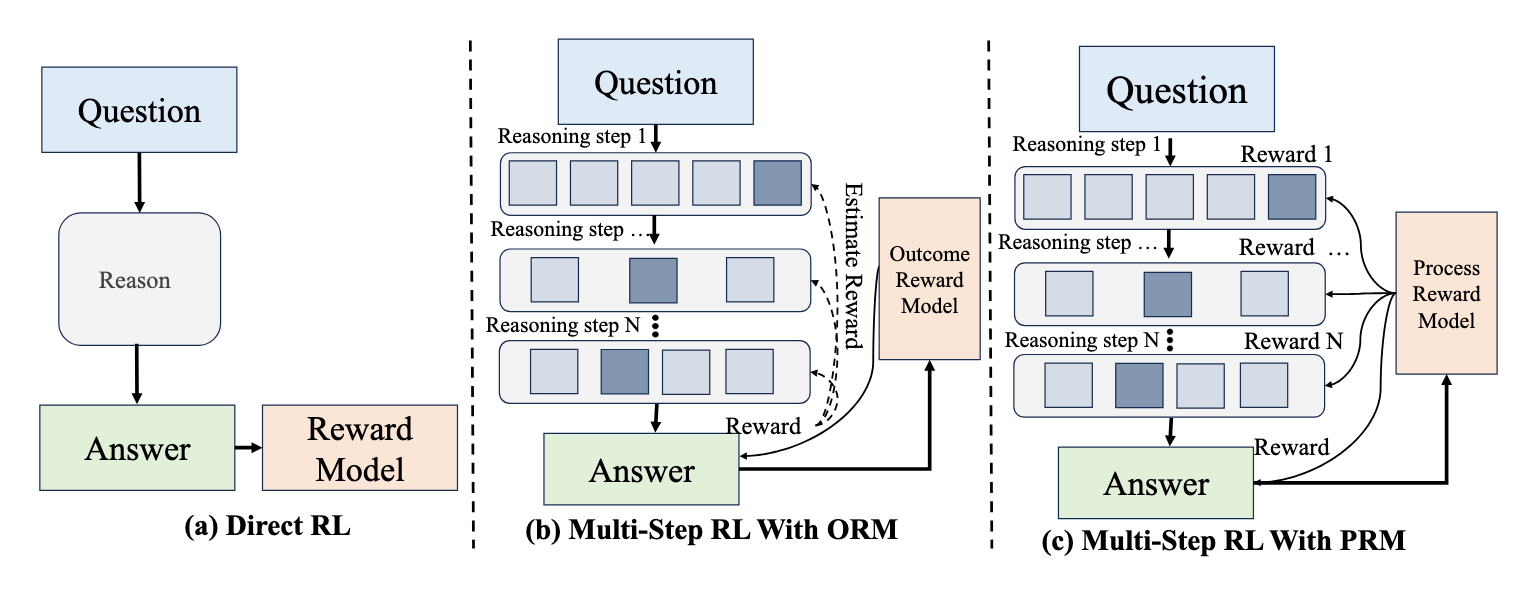
\includegraphics[width=1\textwidth]{images/rl-reward-models}
            \caption{Comparison of different approaches to rewarding models during RL training. The model reasons using chain-of-thought before giving a final answer. Reward models grade the answer and/or the reasoning steps of the model being trained.~\parencite{xu2025largereasoningmodelssurvey}}
        \end{figure}
    \end{frame}
    \begin{frame}
        \begin{figure}
            \begin{columns}
                \begin{column}{0.4\textwidth}
                    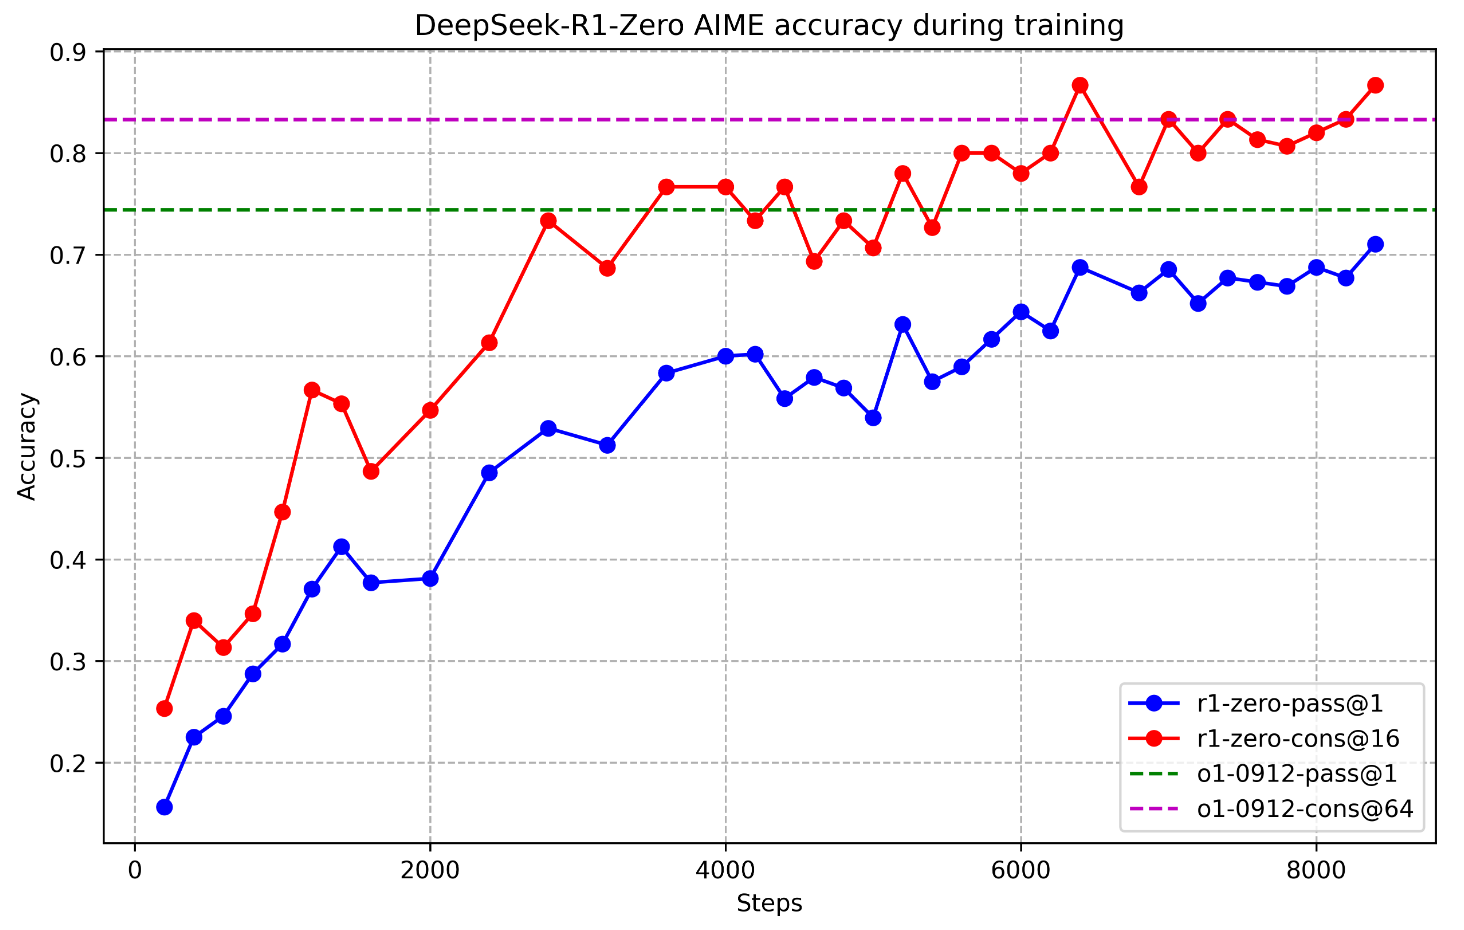
\includegraphics[width=\linewidth]{images/deepseek-r1-zero-aime}
                \end{column}
                \begin{column}{0.45\textwidth}
                    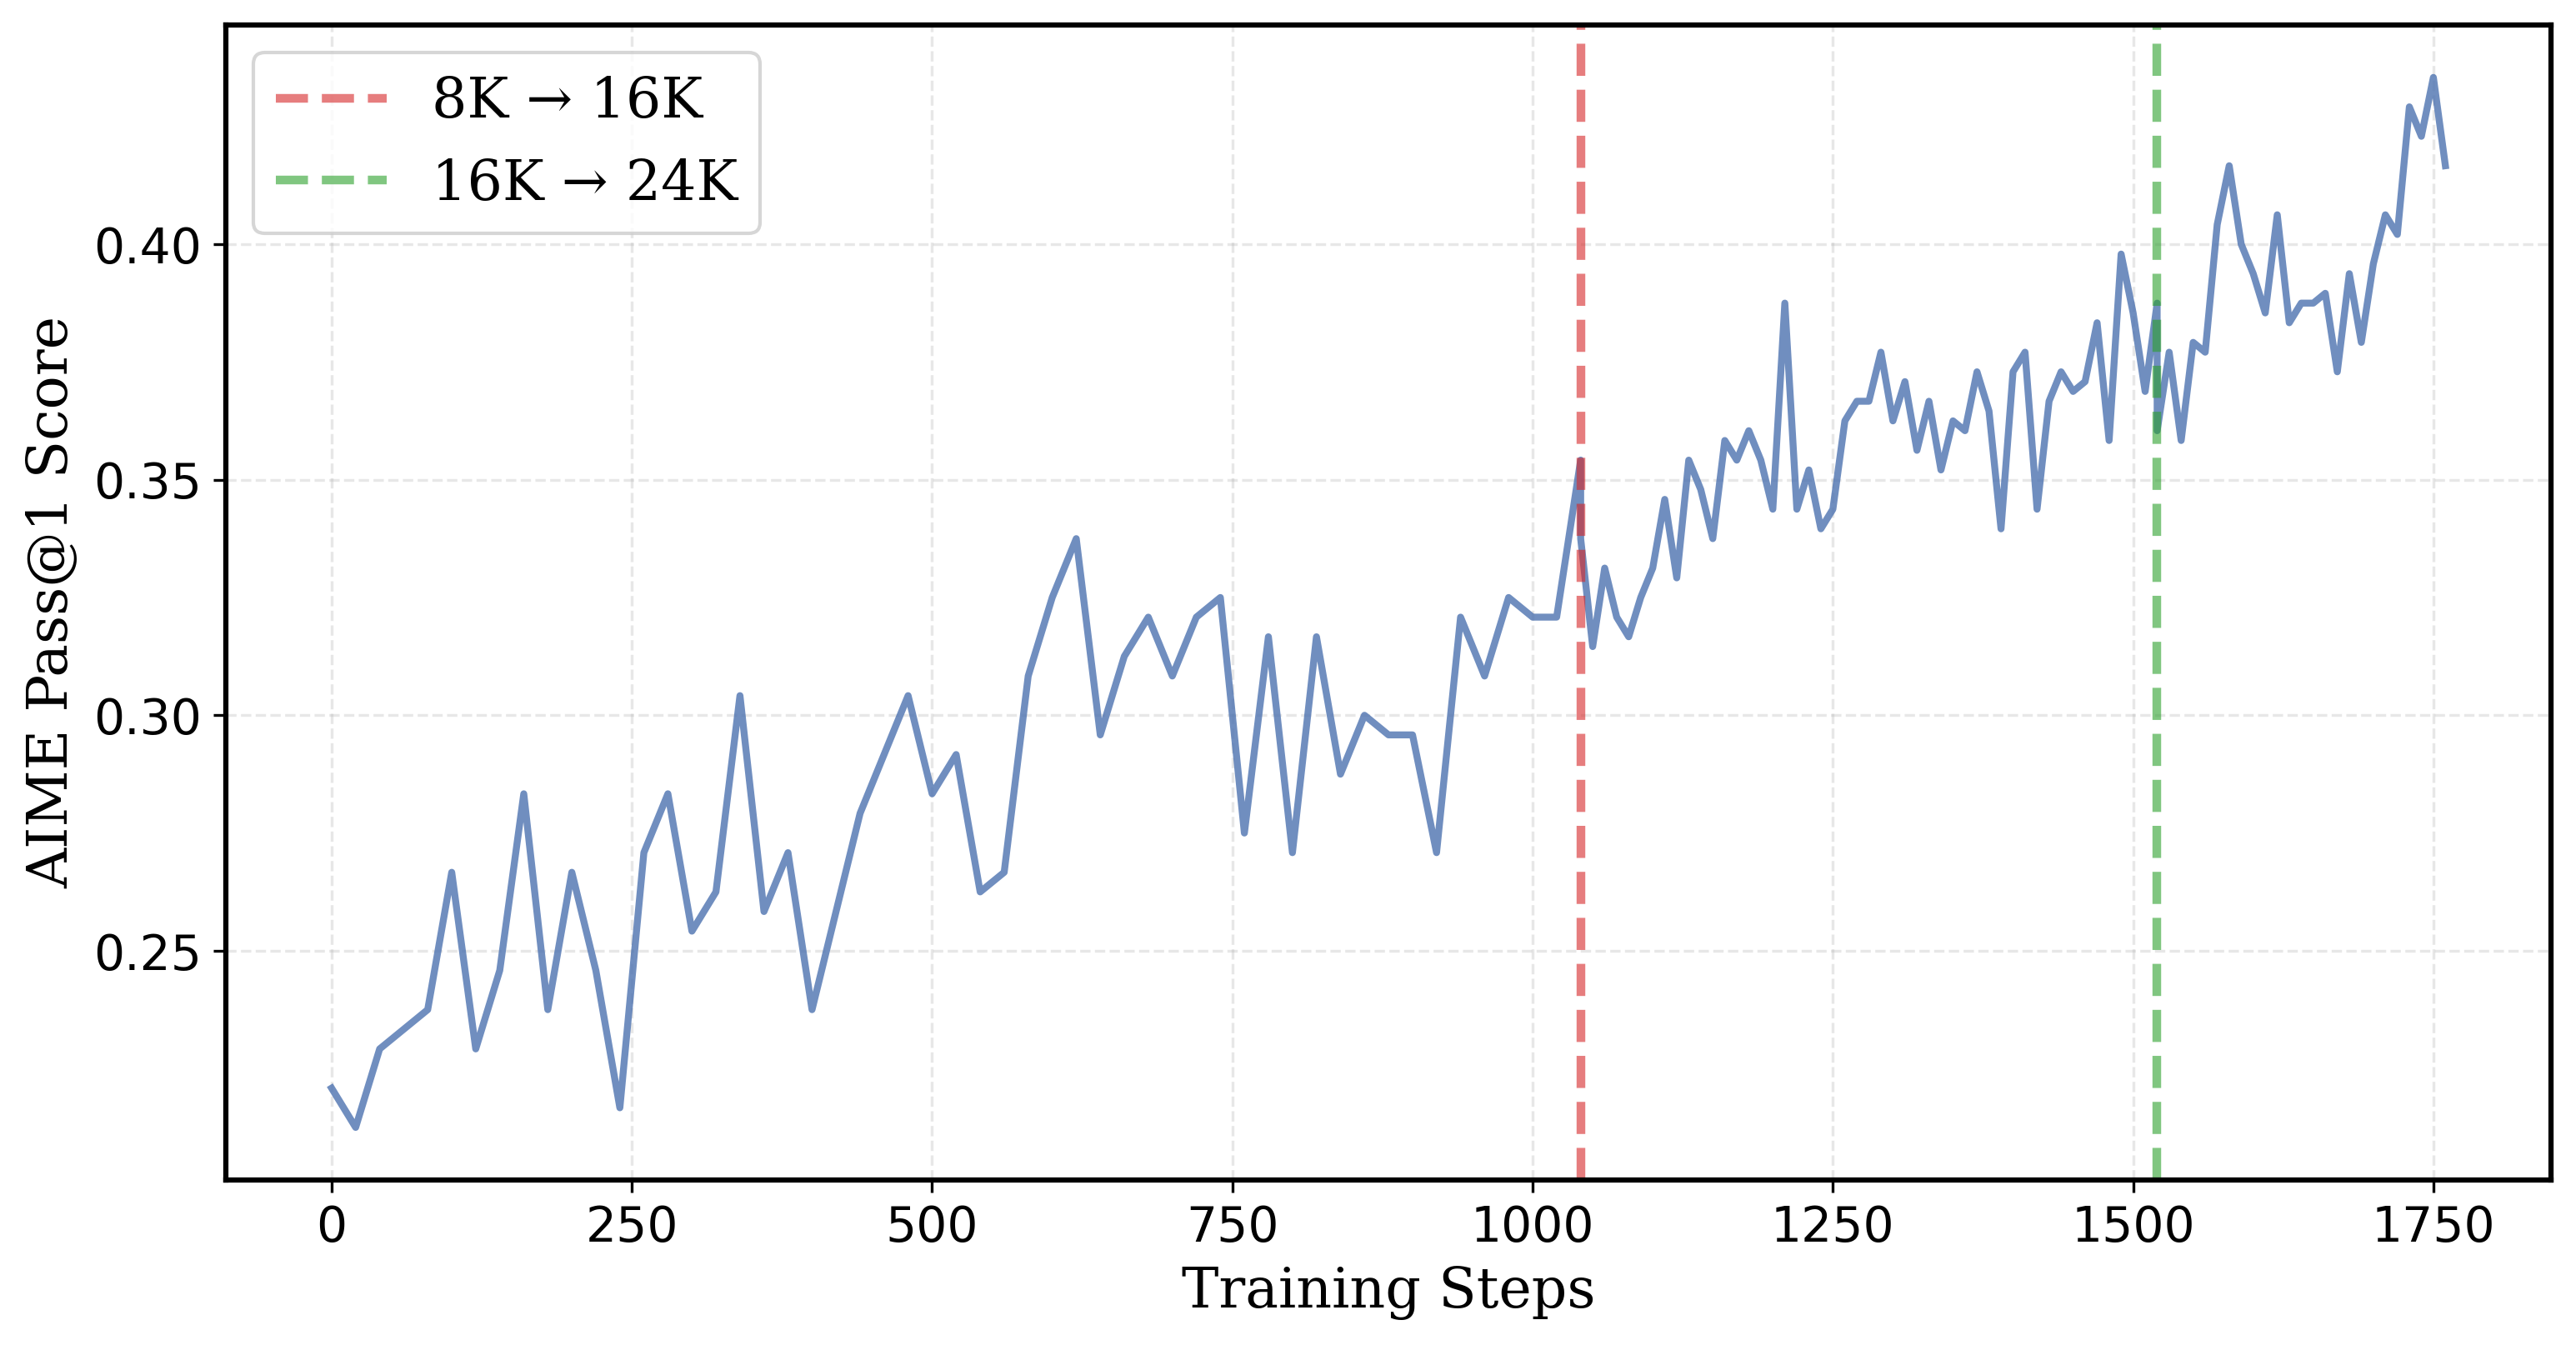
\includegraphics[width=\linewidth]{images/deepscaler-aime}
                \end{column}
            \end{columns}
            \begin{columns}
                \begin{column}{0.4\textwidth}
                    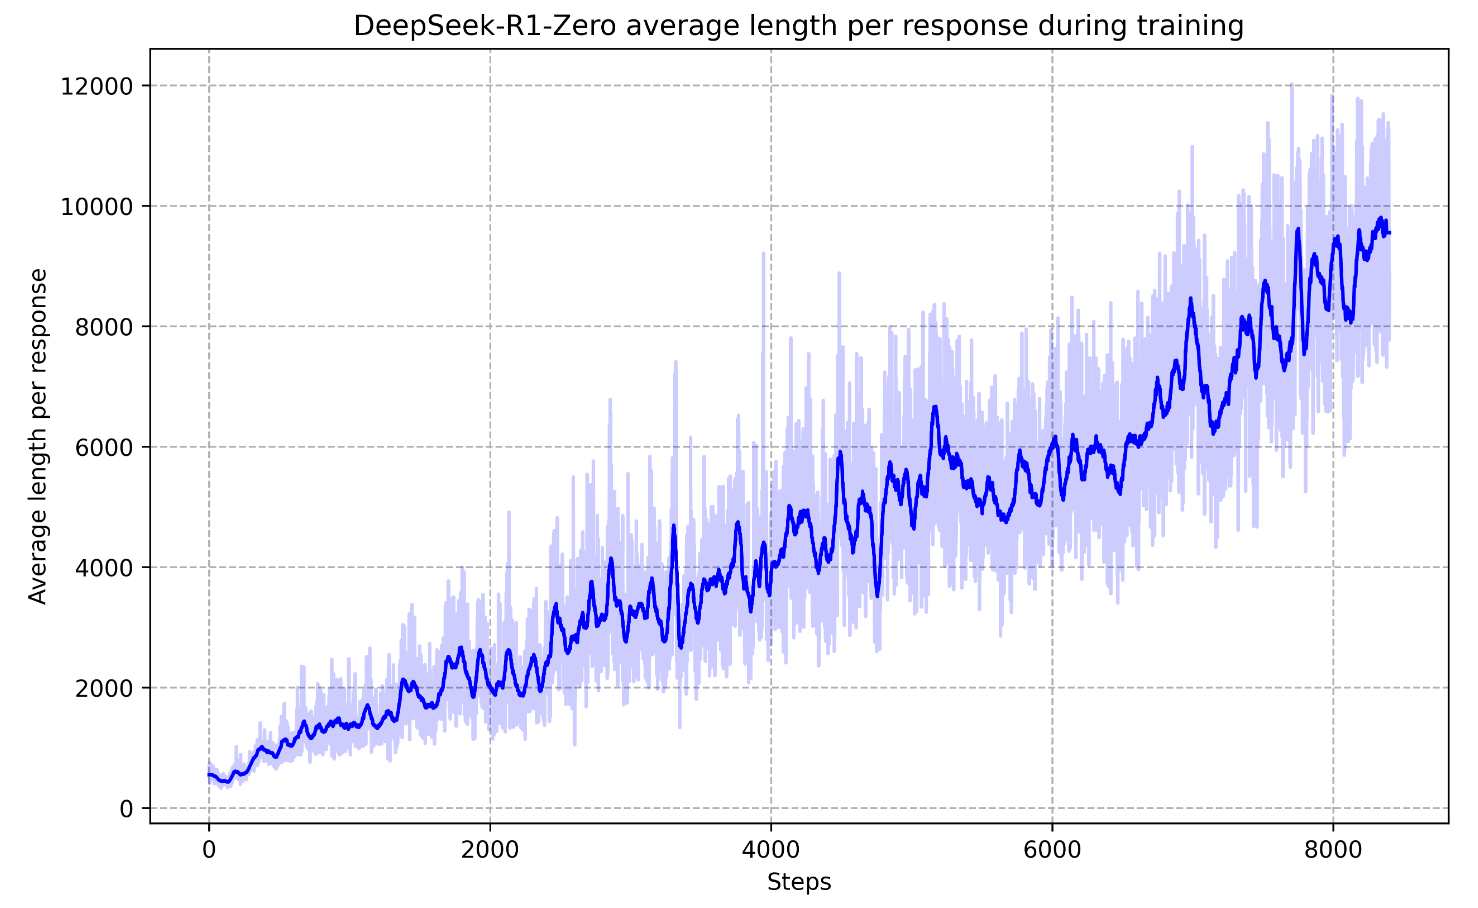
\includegraphics[width=\linewidth]{images/deepseek-r1-zero-response-length}
                \end{column}
                \begin{column}{0.45\textwidth}
                    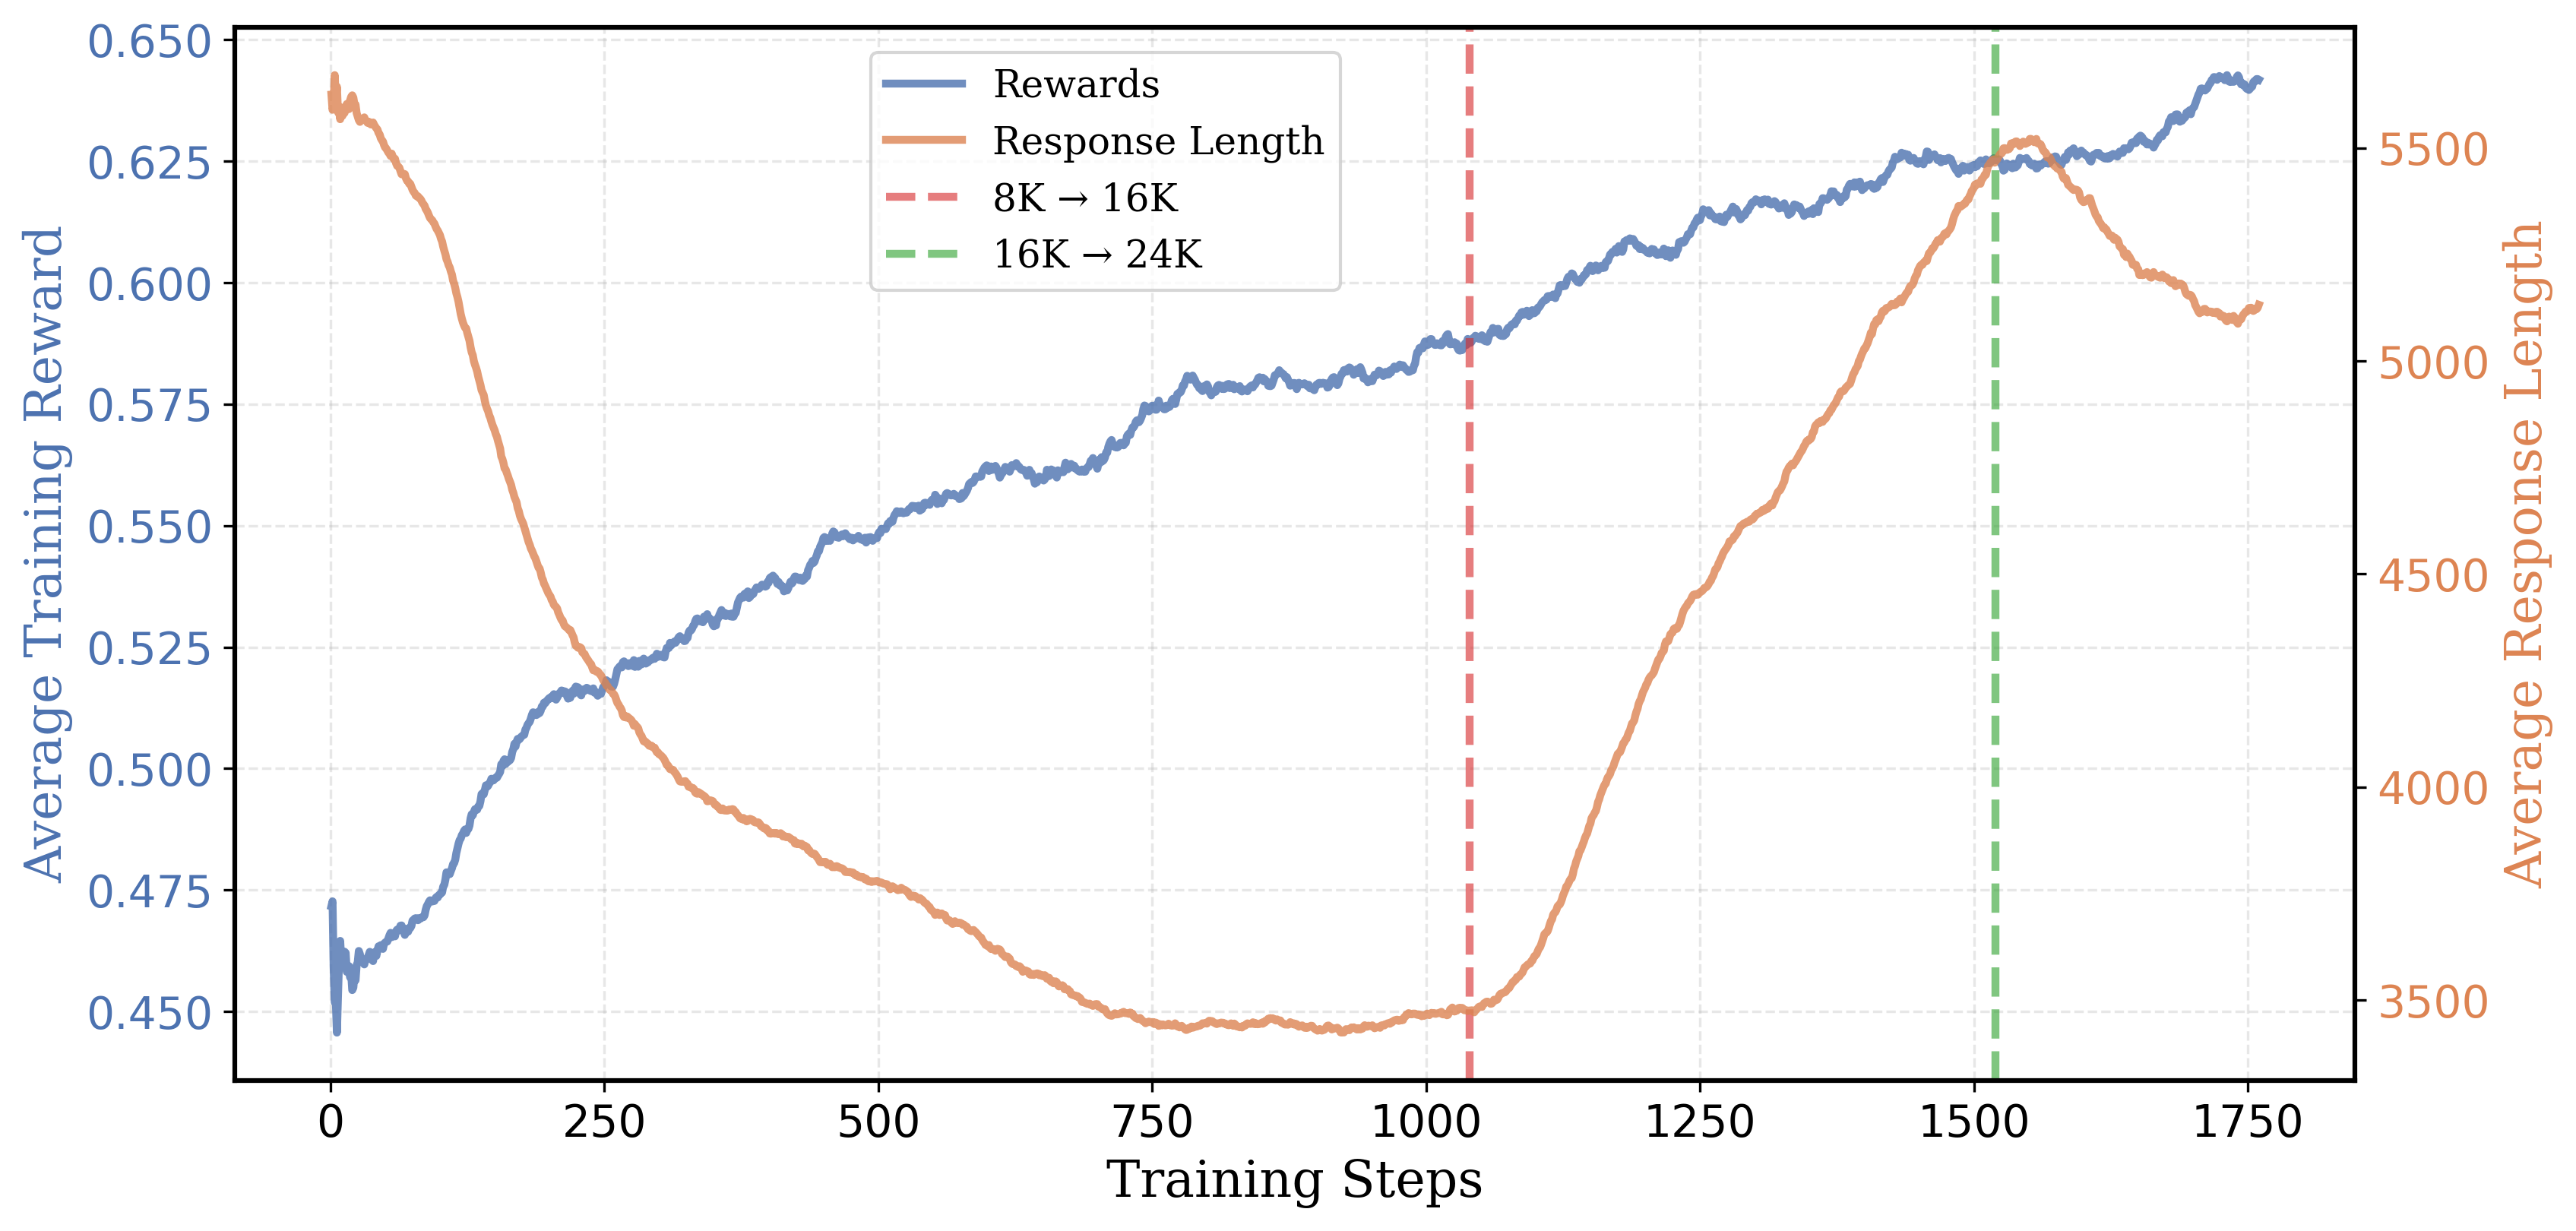
\includegraphics[width=\linewidth]{images/deepscaler-reward-response-length}
                \end{column}
            \end{columns}
            \caption{Accuracy on AIME (top) and response length (bottom) of Deepseek-R1-Zero (left) and DeepScaleR-1.5B (right) during RL training.~\parencite{deepseekai2025, deepscaler2025}}
        \end{figure}
    \end{frame}
        \begin{frame}
        \begin{figure}
            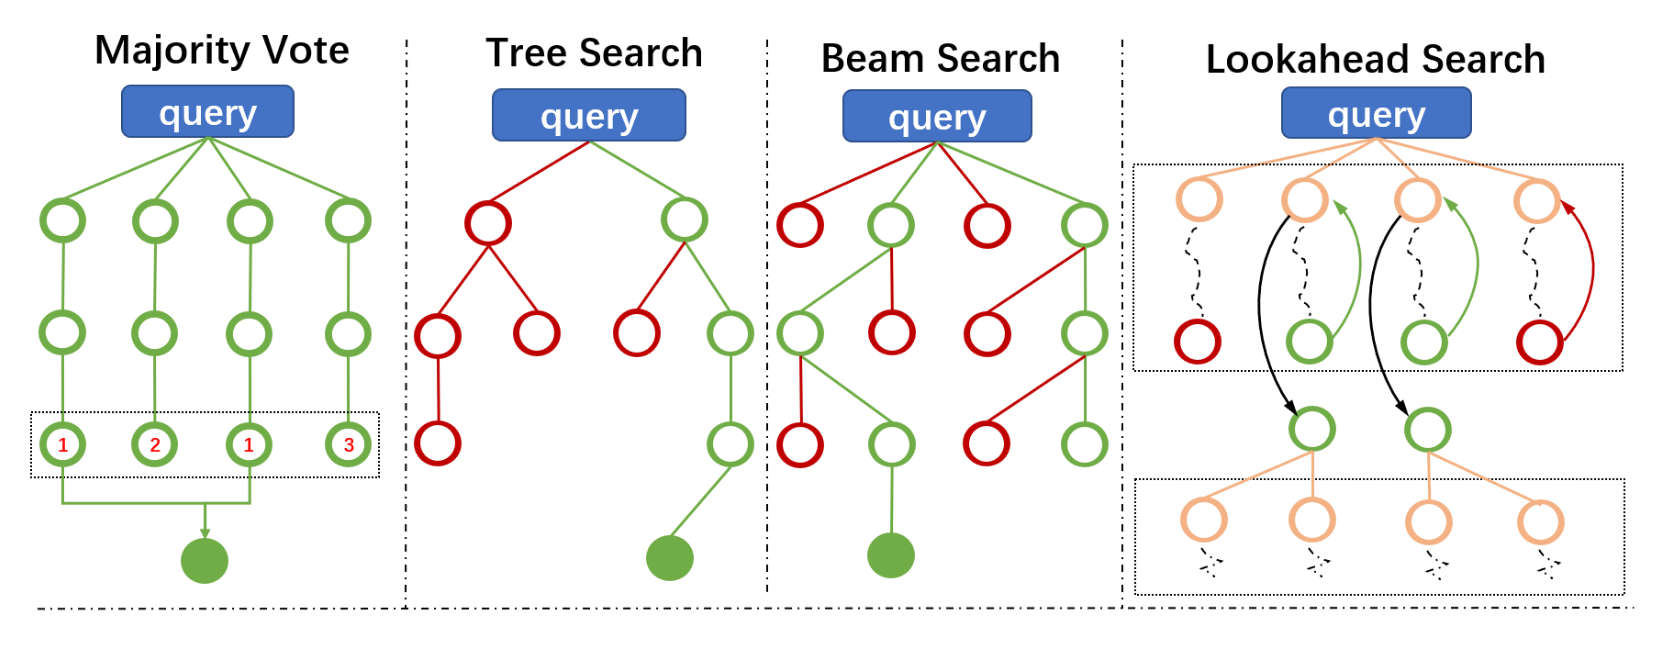
\includegraphics[width=1\textwidth]{images/inference-time-search-algorithms}
            \caption{Comparison of different search algorithms to further scale inference-time compute. Such a method is likely used for the "Pro" mode of OpenAI o1.~\parencite{xu2025largereasoningmodelssurvey}}
        \end{figure}
    \end{frame}
    \begin{frame}
        \frametitle{Reasoning Models Make Big Jumps in Reasoning and Planning}
        \begin{itemize}
            \item Reasoning
            \begin{itemize}
                \item ARC-AGI-Pub~\parencite{chollet_o3_2024}
                \begin{itemize}
                    \item Semi-Private Eval: \alert{76\% (OpenAI o3)} vs.\ 77\% (MTurkers)
                    \item Public Eval: \alert{83\% (OpenAI o3)} vs.\ 64\% (Humans)~\parencite{legris2024harcrobustestimatehuman}
                \end{itemize}
            \end{itemize}
            \item Planning
            \begin{itemize}
                \item PlanBench~\parencite{valmeekam2024llmscantplanlrms}
                \begin{itemize}
                    \item Mystery Blocksworld (0-shot): \alert{53\% (OpenAI o1-preview)}
                \end{itemize}
            \end{itemize}
            \item Autonomy
            \begin{itemize}
                \item OSWorld~\parencite{OSWorld}
                \begin{itemize}
                    \item 38\% (OpenAI CUA) vs.\ 72\% (Humans)
                \end{itemize}
                \item GAIA~\parencite{mialon2023gaia}
                \begin{itemize}
                    \item 67\% (OpenAI Deep Research)~\parencite{openai_deep_research_2025} vs.\ 92\% (Humans)
                \end{itemize}
            \end{itemize}
        \end{itemize}
    \end{frame}
    \begin{frame}
        \frametitle{How Far Have Reasoning Models Been Scaled so Far?}
        \begin{itemize}
            \item DeepSeek R1 is estimated to have only used 6.1e23 FLOP during RL training on 2 trillion tokens~\parencite{erdil_deepseek_2025}
            \begin{itemize}
                \item 15,405 H800 days or roughly 1/34th of the compute used to train GPT-4
                \item If current compute scaling trends can be sustained, a training run requiring more than 300,000x the compute would be possible in 2030
            \end{itemize}
            \item It is unknown what type of data and how much data was used for training any state-of-the-art reasoning model
            \item State-of-the-art reasoning models like OpenAI o3-mini and DeepSeek R1 generate up to several thousands of reasoning tokens for each response
            \begin{itemize}
                \item Current state-of-the-art language models support context lengths ranging from 128,000 to 2,000,000 tokens
            \end{itemize}
        \end{itemize}
    \end{frame}
    \begin{frame}
        \frametitle{Could Reinforcement Learning Solve Autonomy?}
        \begin{itemize}
            \item AI agents aim to make AI able to act in digital environments like a virtual machine or a web browser to solve multi-step tasks
            \item AI agents currently still have major issues like difficulty interacting with GUIs, difficulty solving long-horizon tasks and a lack of commonsense and social skills~\parencite{xu2024theagentcompanybenchmarkingllmagents}
            \item Applying reinforcement learning to AI agents with verifiers checking the final results of multi-step tasks might be a promising approach~\parencite{pan2024trainingsoftwareengineeringagents}
            \item The tasks and the environments might be human-made or even AI-generated~\parencite{hu2024agentgenenhancingplanningabilities} and need to overcome the simulation-to-reality gap
        \end{itemize}
    \end{frame}
    \begin{frame}
        \begin{figure}
            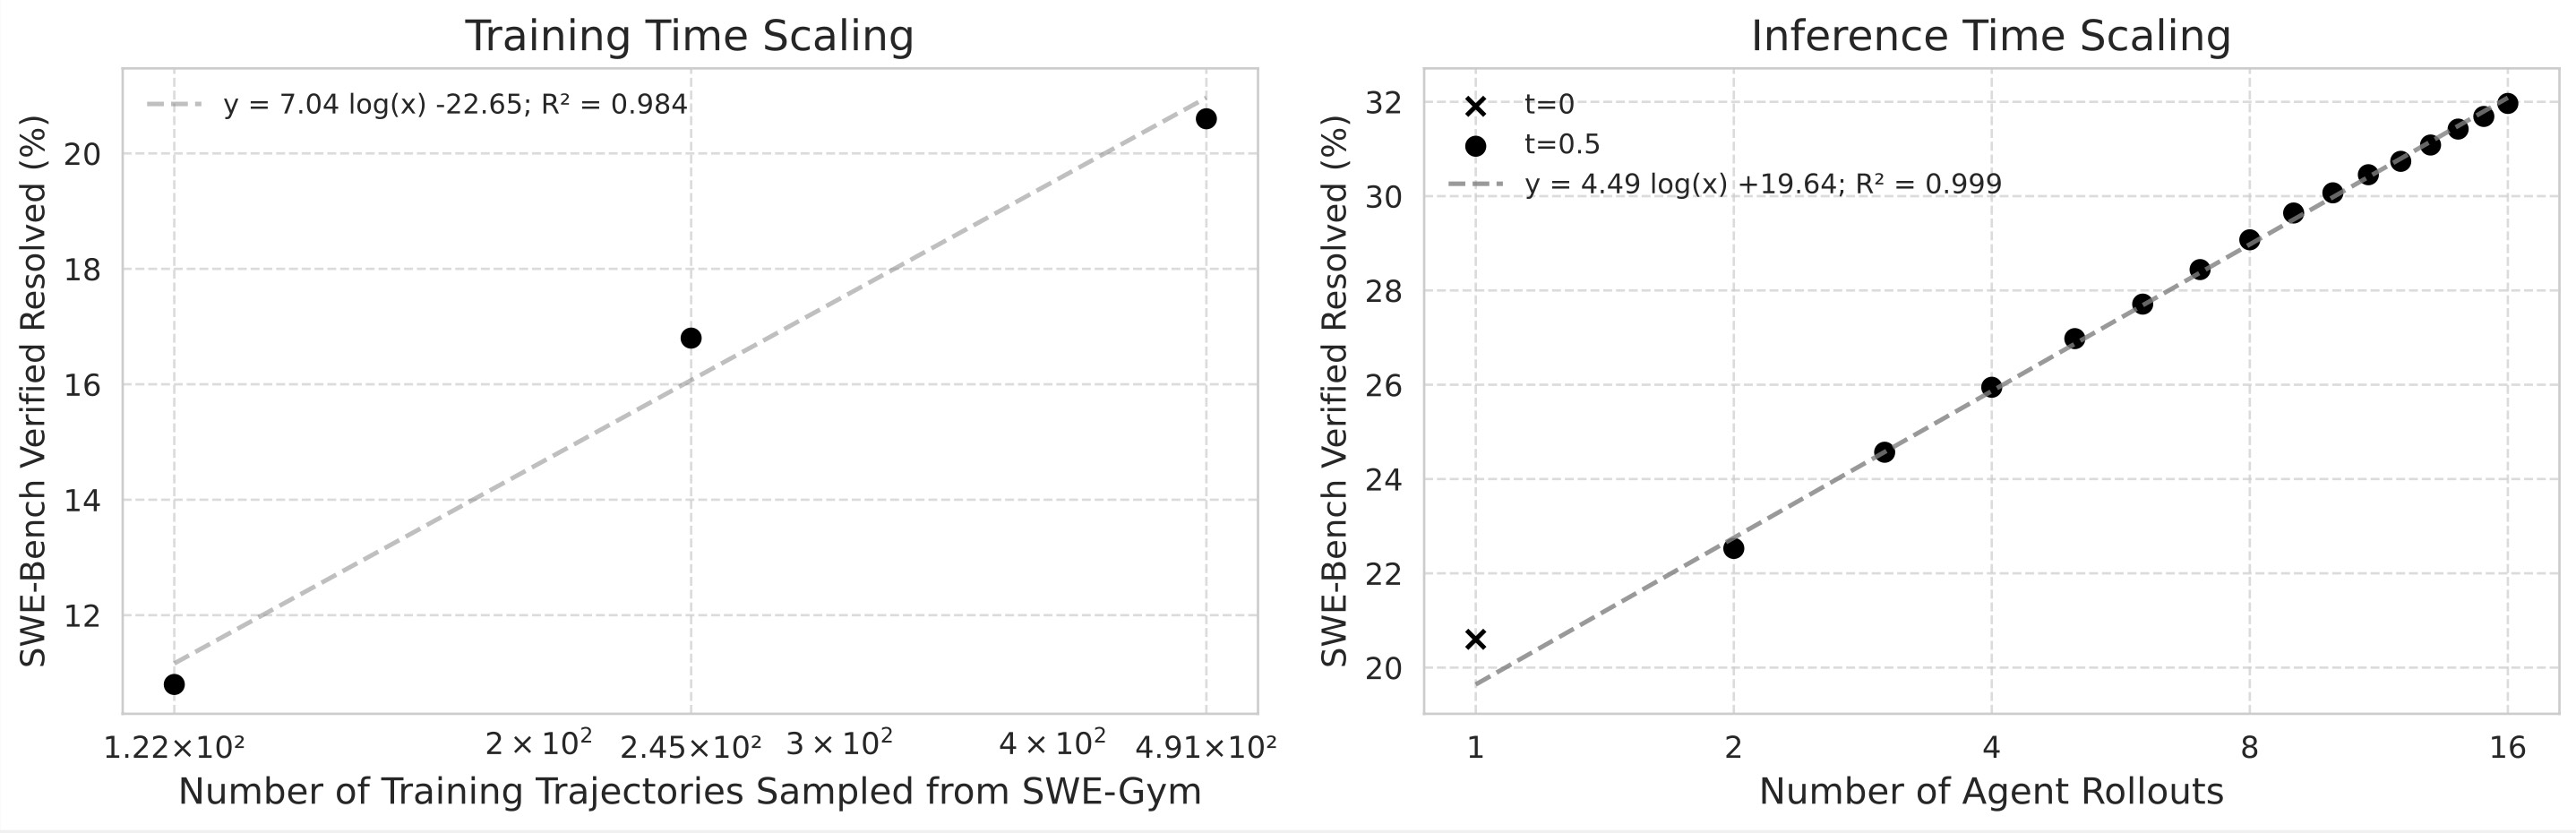
\includegraphics[width=1\textwidth]{images/swegym-agent-scaling}
            \caption{Log-linear increase in performance of software engineering agents through training compute scaling and inference compute scaling. The agents were trained on 491 agent trajectories sampled from agents solving tasks in the SWE-Gym training environment.~\parencite{pan2024trainingsoftwareengineeringagents} Large-scale agent training, especially the potential of reinforcement learning by scaling chain-of-throught reasoning, still has to be properly researched.}
        \end{figure}
    \end{frame}
    \begin{frame}
        \frametitle{Data and Architecture: In a Nutshell}
        \begin{itemize}
            \item Language model training involves three distinct phases: pre-training, instruction-tuning, and now reinforcement learning (RL) to scale reasoning.
            \item The industry faces a ``data wall'' within five years at current scaling trends.
            \item AI-generated training data is increasingly used but brings risks, making verification of generated content crucial for maintaining quality.
            \item Reasoning models represent a fundamental shift, enabling breakthrough performance in areas where previous models significantly underperformed humans.
            \item These models require more inference compute but may help overcome the looming ``data wall'' since RL training appears more data-efficient than pre-training.
            \item Despite impressive gains in reasoning, planning, math and coding, reasoning models have barely been scaled so far due to them only being discovered recently.
            \item The potential application of RL to agent training could transform AI autonomy, though significant challenges and uncertainties remain.
        \end{itemize}
    \end{frame}


    \section{Finance}
    \begin{frame}
        \frametitle{How Much Would Autonomous Generalist AI Be Worth?}
        \begin{itemize}
            \item Imagine a system that can autonomously complete basically any job that a human can perform on a computer.
            \item Let's make a simple calculation to calculate how much such a system might be worth:
            \begin{itemize}
                \item Let's very conservatively assume that such an AI could perform work equivalent to 1\% of world GDP (imagine a 1\% increase in global productivity).
                \item Such AI would therefore make around \$1.15 trillion annually (1\% of world GDP).
                \item A tech company with such revenues could be valued at \$6.3 trillion (using current P/S ratio of the NASDAQ 100).
            \end{itemize}
            \item Even using very conservative estimates, it's clear that such AI would be worth an astronomical amount.
            \item Investing trillions of dollars into AI research and development seems worth it once it seems possible that autonomous generalist AI can be achieved.
        \end{itemize}
    \end{frame}
    \begin{frame}
        \frametitle{How Much Do Leading Tech Companies Make?}
        \begin{table}
            \centering
            \begin{tabular}{llrr}
                \toprule
                Company   & Country & Revenue & Net Income \\
                \midrule
                Amazon    & USA     & \$514B  & -\$3B      \\
                Apple     & USA     & \$394B  & \$100B     \\
                Google    & USA     & \$283B  & \$60B      \\
                Microsoft & USA     & \$198B  & \$73B      \\
                Alibaba   & China   & \$135B  & \$10B      \\
                Meta      & USA     & \$117B  & \$23B      \\
                ByteDance & China   & \$85B   & \$25B      \\
                Tencent   & China   & \$82B   & \$28B      \\
                SAP       & Germany & \$31B   & \$2B       \\
                Baidu     & China   & \$18B   & \$1B       \\
                \bottomrule
            \end{tabular}
            \caption{Revenue and net income of selected technology companies in 2022}
        \end{table}
    \end{frame}
    \begin{frame}
        \frametitle{How Much Are Leading Tech Companies Spending Now?}
        \begin{table}
            \centering
            \begin{tabular}{llrrrr}
                \toprule
                Company           & Country     & Q1 2023       & Q3/Q4 2024     &                &                \\
                \midrule
                \alert{Amazon}    & \alert{USA} & \alert{\$57B} & \alert{\$111B} & \alert{+\$55B} & \alert{+96\%}  \\
                Apple             & USA         & \$12B         & \$12B          & +\$0B          & +1\%           \\
                \alert{Google}    & \alert{USA} & \alert{\$25B} & \alert{\$57B}  & \alert{+\$32B} & \alert{+127\%} \\
                \alert{Microsoft} & \alert{USA} & \alert{\$26B} & \alert{\$63B}  & \alert{+\$37B} & \alert{+139\%} \\
                Alibaba           & China       & \$1B          & \$10B*         & +\$8B          & +560\%         \\
                \alert{Meta}      & \alert{USA} & \alert{\$27B} & \alert{\$58B}  & \alert{+\$30B} & \alert{+111\%} \\
                ByteDance         & China       & ?             & ?              & ?              & ?              \\
                Tencent           & China       & \$2B          & \$14B*         & +\$12B         & +497\%         \\
                SAP               & Germany     & €1B           & €1B            & +€0B           & +5\%           \\
                Baidu             & China       & \$1B          & \$1B*          & +\$0B          & +24\%          \\
                \bottomrule
            \end{tabular}
            \caption{Annualized capital expenditures (excluding leases) of selected technology companies}
        \end{table}
    \end{frame}
    \begin{frame}
        \frametitle{How Much Are Leading Tech Companies Planning to Spend?}
        \begin{itemize}
            \item Amazon expects total capital expenditures (capex) in 2025 to be at around \$105 billion with ``the vast majority of that capex spend is on AI for AWS'' for this ``once-in-a-lifetime type of business opportunity''.~\parencite{cnbc_amazon_2025}
            \item Google expects total capex to ``continue to increase in 2025'', hitting \$75 billion with the majority of it for data centers.~\parencite{data_center_dynamics_google_2025}
            \item Microsoft is ``on track to invest approximately \$80 billion'' on AI infrastructure in fiscal year 2025 while noting ``in many ways, artificial intelligence is the electricity of our age''.~\parencite{microsoft_golden_2025}
            \begin{itemize}
                \item Equivalent to 29\% of total expected revenue in 2025~\parencite{yahoo_finance_microsoft_2025}
            \end{itemize}
            \item Meta expects total capex in 2025 to be ``in the range of \$60 billion to \$65 billion'' while noting the ``hundreds of billions of dollars that we will invest into AI infrastructure over the long term''~\parencite{meta_earnings_call_2025}
            \item For comparison: Peak annual cost of Apollo and related programs was \$48 billion (1965, adjusted for inflation)~\parencite{planetary_society_how_2019}
        \end{itemize}
    \end{frame}
    \begin{frame}
        \frametitle{Finance: In a Nutshell}
        \begin{itemize}
            \item Amazon, Google, Microsoft and Meta are each making their most expensive bet yet with each of them roughly doubling their total capital expenditures in the past two years in order to spend unprecedented amounts on AI infrastructure.
            \item The annualized spending on AI infrastructure of each of these companies is now reaching the annual costs of the most expensive megaprojects ever (such as the Apollo program).
        \end{itemize}
    \end{frame}


    \section{Chips}
    \begin{frame}
        \frametitle{Chips Used For Training AI in the Past, Present and Future}
        \begin{itemize}
            \item Graphics Cards (2012-2016)
            \begin{itemize}
                \item \textcite{NIPS2012_c399862d} championed the use of graphics cards to train their groundbreaking AlexNet model
                \item Speeds up calculations with parallel computing and faster memory
            \end{itemize}
            \item AI Accelerators (2015-present)
            \begin{itemize}
                \item The first AI accelerators included Google's TPU v1 and NVIDIA's P100
                \item Designed for ML and HPC, usually featuring tensor cores, support for lower-precision arithmetic, high-bandwidth memory (HBM) and 2.5D packaging
            \end{itemize}
            \item ASICs and In-Memory Computing (2019-present)
            \begin{itemize}
                \item Examples include the Cerebras WSE~\parencite{cerebras_wse_3_2024}, the Groq LPU~\parencite{groq_groqrack_2024} (only for inference) and the Etched Sohu~\parencite{etched_announcement_2024} (only for inference)
            \end{itemize}
            \item Photonic Computing (Research Stage)
            \item Analog Neuromorphic Computing (Research Stage)
        \end{itemize}
    \end{frame}
    \begin{frame}
        \begin{figure}
            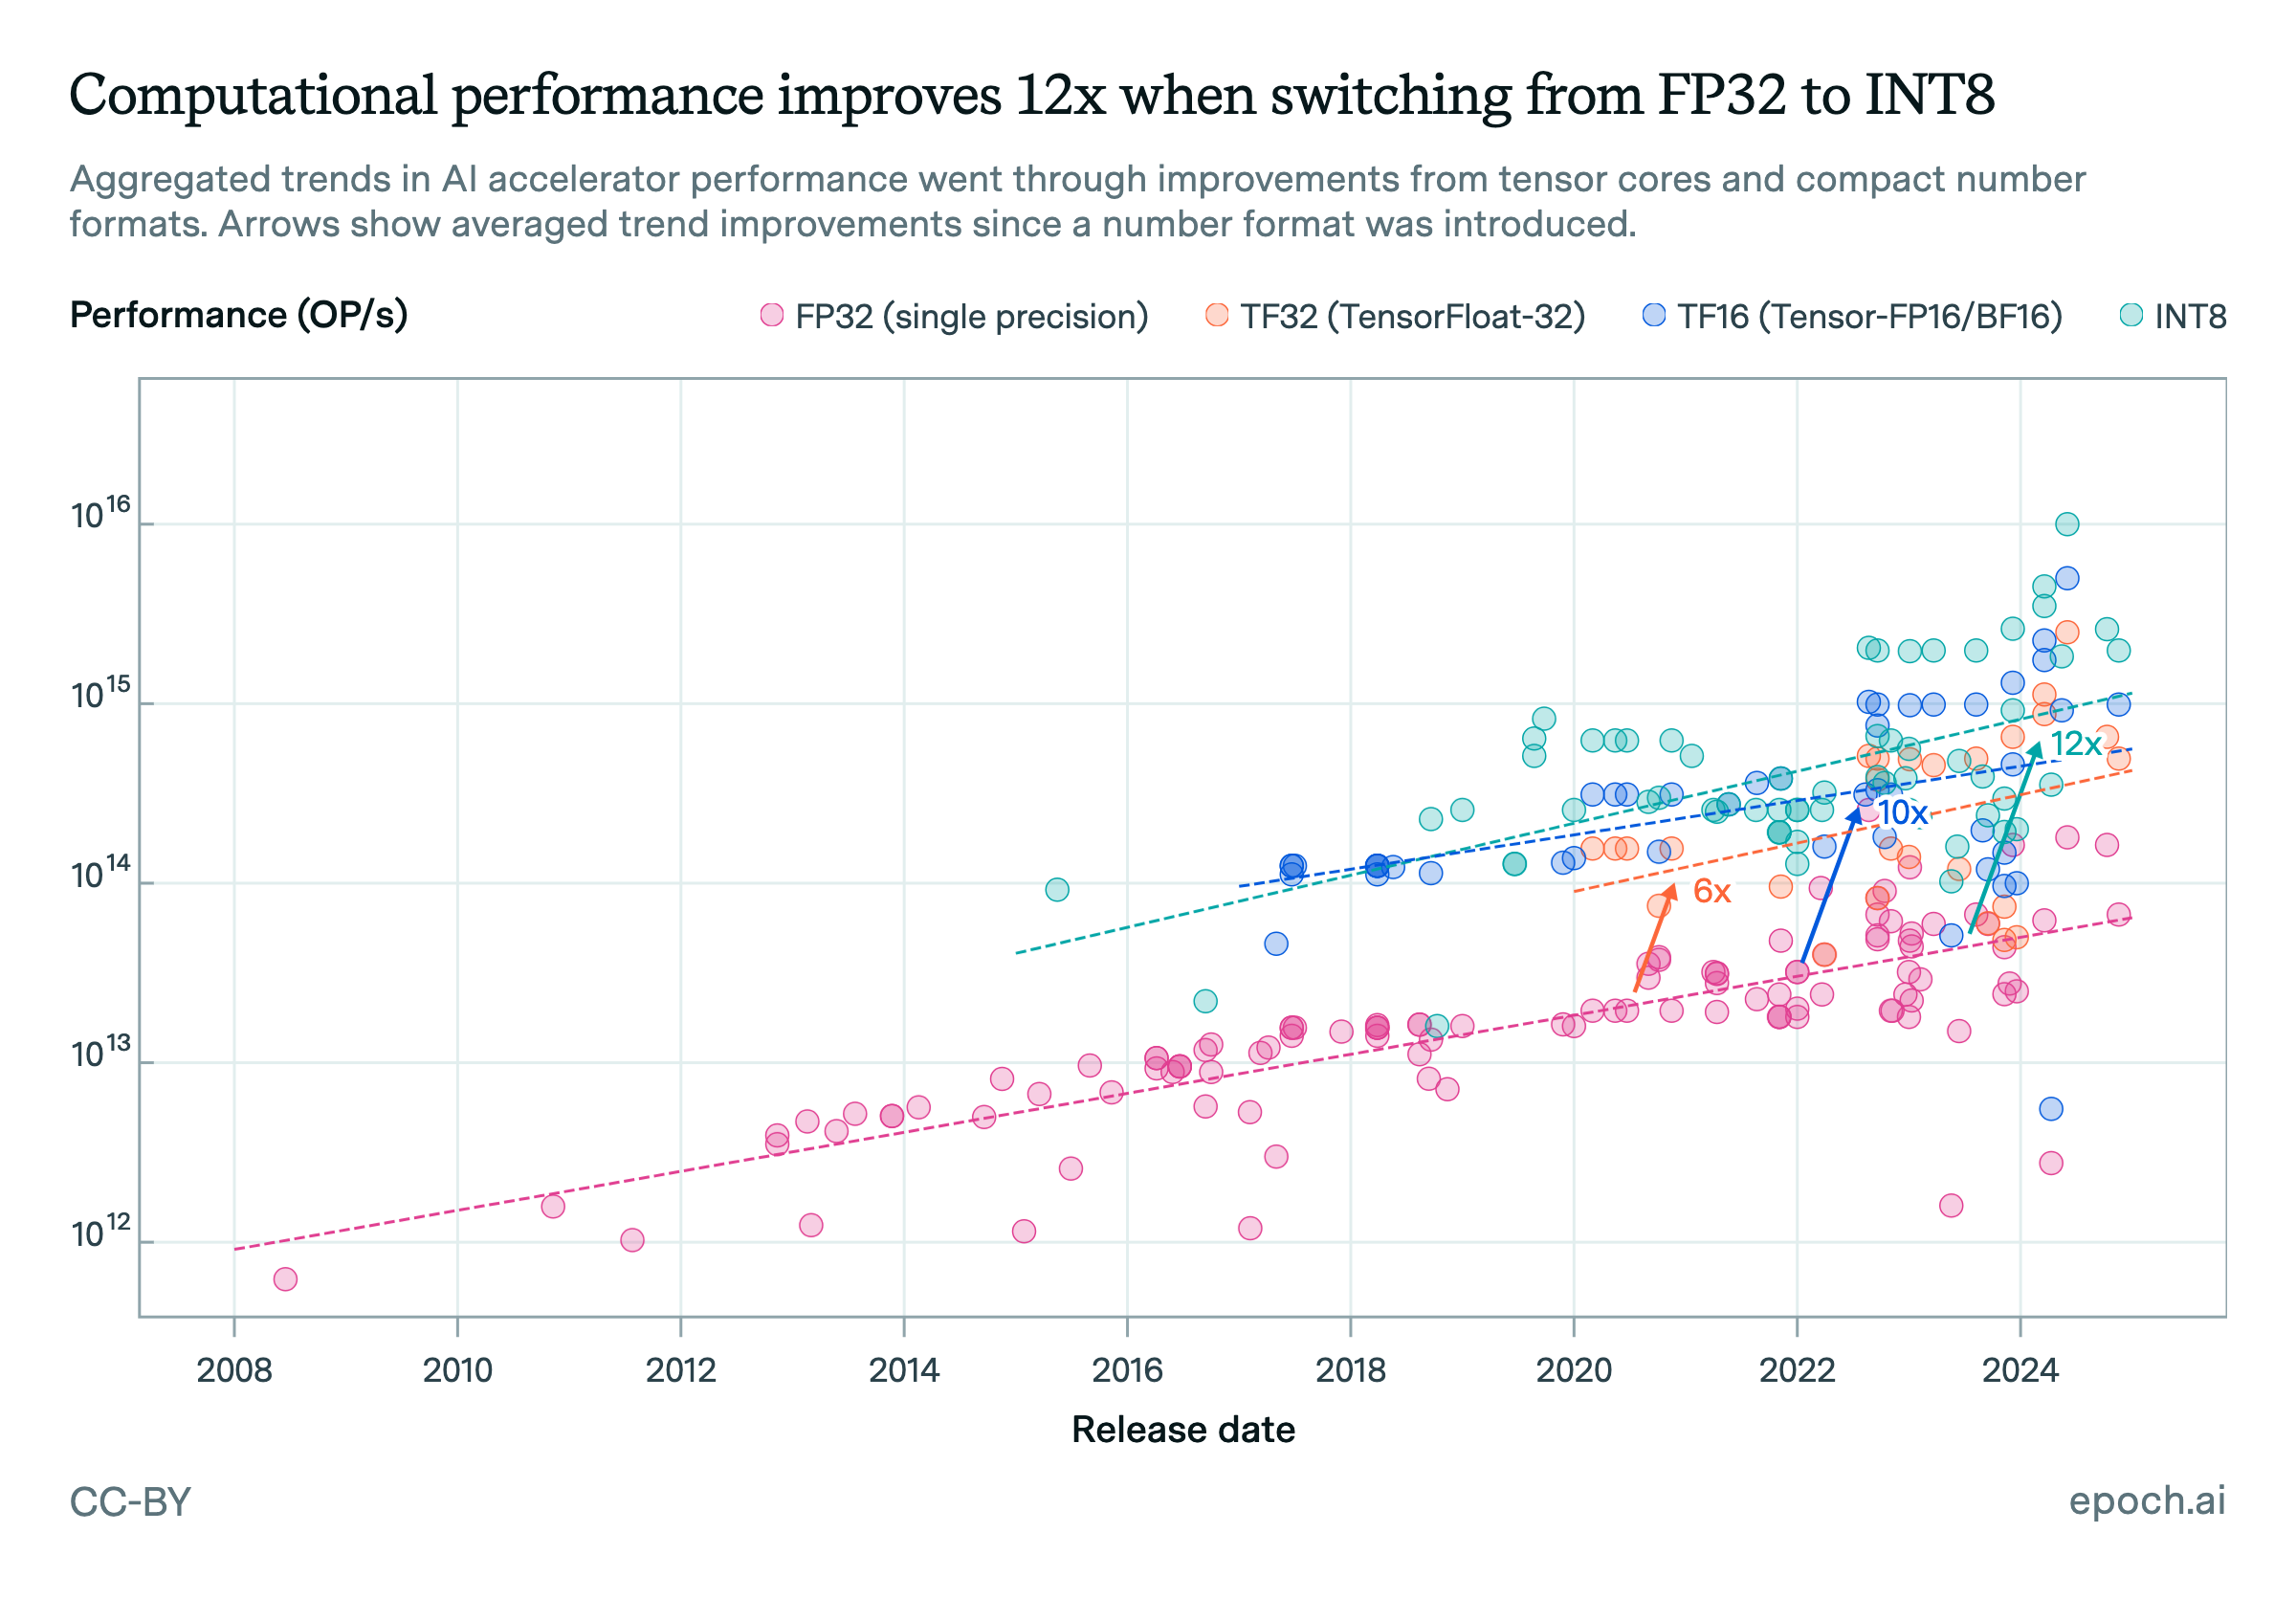
\includegraphics[height=0.45\textwidth]{images/hardware-performance-trend}
            \caption{AI accelerator performance is increasing rapidly, especially when including support for lower-precision arithmetic. The NVIDIA B200 (released in 2024) using FP8 offers 2,812x the peak performance of the NVIDIA GeForce GTX 580 (released in 2010) using FP32 (used by \textcite{NIPS2012_c399862d} to train AlexNet).~\parencite{epoch_ai_performance_2024}}
        \end{figure}
    \end{frame}
    \begin{frame}
        \frametitle{NVIDIA: King of the AI Hardware Market}
        \begin{itemize}
            \item Dominates the global AI hardware market, selling the overwhelming majority of AI accelerators
            \item 10x data center revenue growth in just two years
            \item Big profit margins on AI accelerators (produced for thousands of dollars, sold for tens of thousands of dollars)
            \item Ramped up production of Hopper GPUs during 2023 and 2024
            \item Currently ramping up production of the new Blackwell GPUs which are sold out for the next 12 months.~\parencite{tweaktown_nvidia_2024}
            \begin{itemize}
                \item The B200 offers roughly a 2.5x performance improvement over the H100.
                \item The new NVL72 racks connect 72 GPUs, ideal for large-scale AI training.
            \end{itemize}
        \end{itemize}
    \end{frame}
    \begin{frame}
        \begin{figure}
            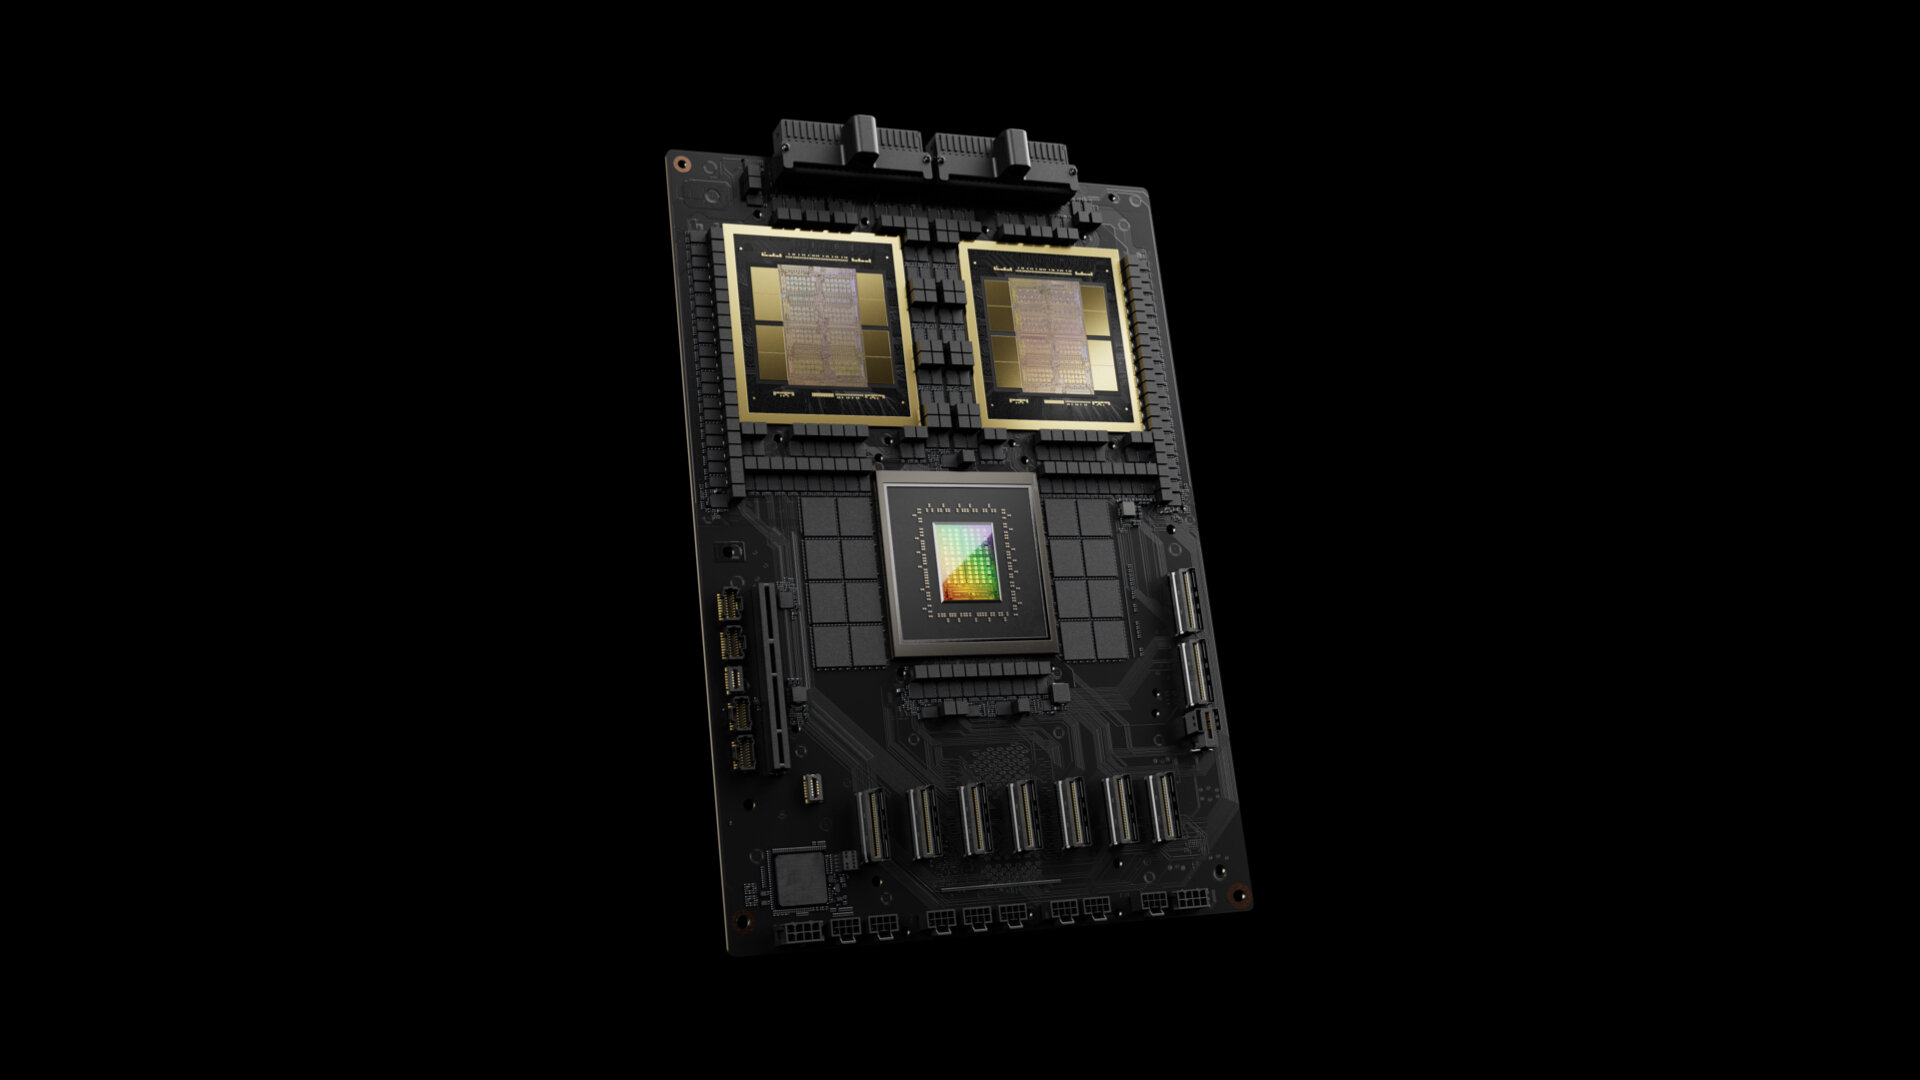
\includegraphics[height=0.5\textwidth]{images/gb200-superchip}
            \caption{NVIDIA GB200 ``superchip'' featuring 2 GPUs, 1 CPU, 384 GB HBM3e memory, 480 GB LPDDR5X memory and 2700 W TDP}~\parencite{nvidia_gb200_nvl72_2025}
        \end{figure}
    \end{frame}
    \begin{frame}
        \begin{figure}
            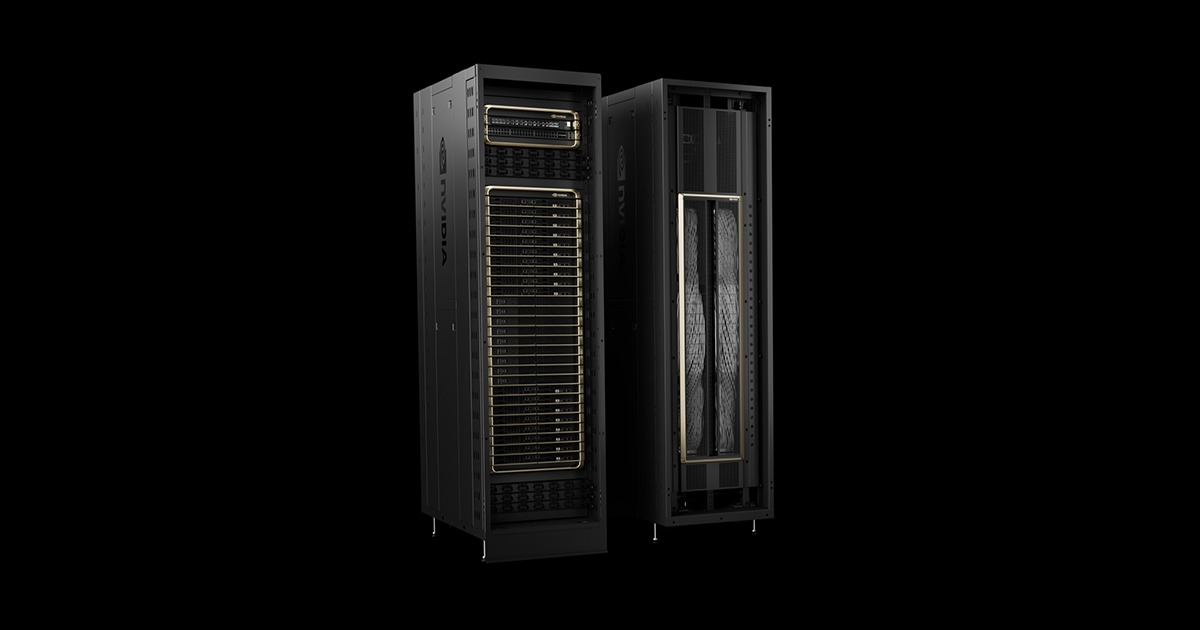
\includegraphics[height=0.5\textwidth]{images/gb-nvl72-og}
            \caption{Two NVIDIA GB200 NVL72 racks, each featuring 72 GPUs, 36 CPUs, 13.5 TB HBM3e memory, 17 TB LPDDR5X memory and 120 kW TDP}~\parencite{nvidia_gb200_nvl72_2025}
        \end{figure}
    \end{frame}
    \begin{frame}
        \begin{figure}
            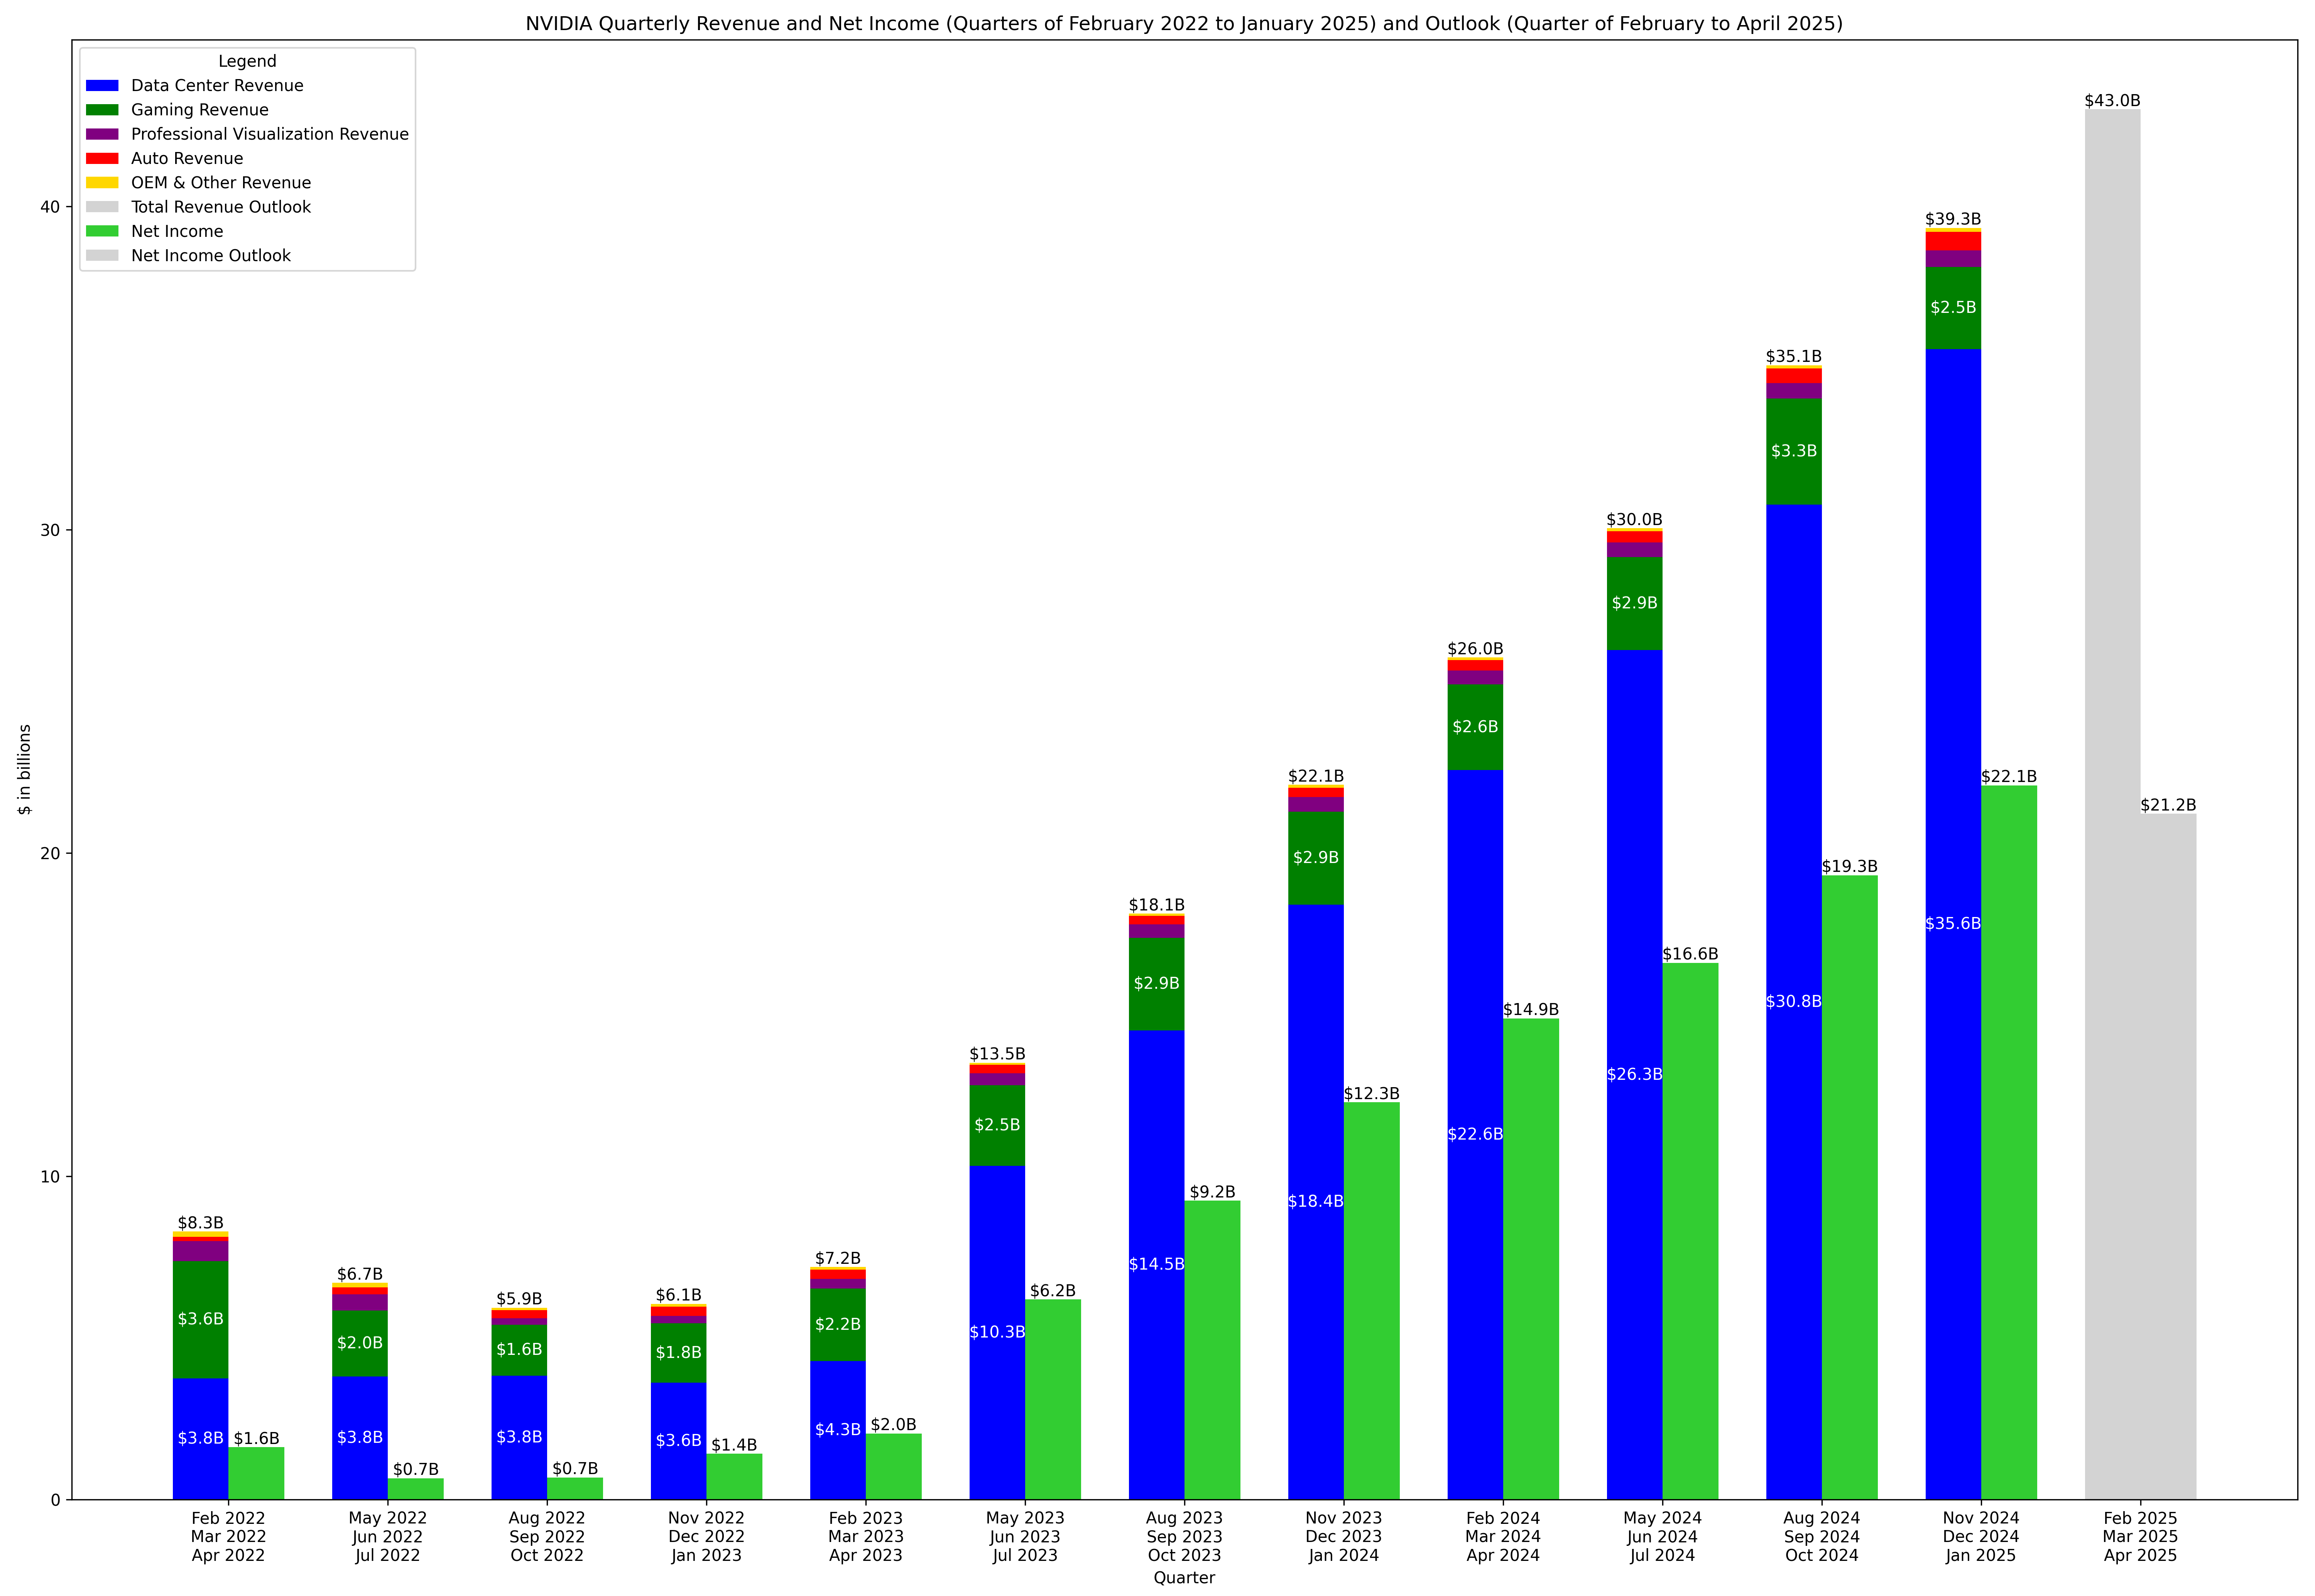
\includegraphics[height=0.5\textwidth]{images/nvidia-revenue}
            \caption{NVIDIA's quarterly data center revenue increased 10-fold from \$3.6B in Q4 2022 to \$35.6B in Q4 2024. In the same time, total profits increased 15-fold from \$1.4B to \$22.1B}
        \end{figure}
    \end{frame}
    \begin{frame}
        \begin{figure}
            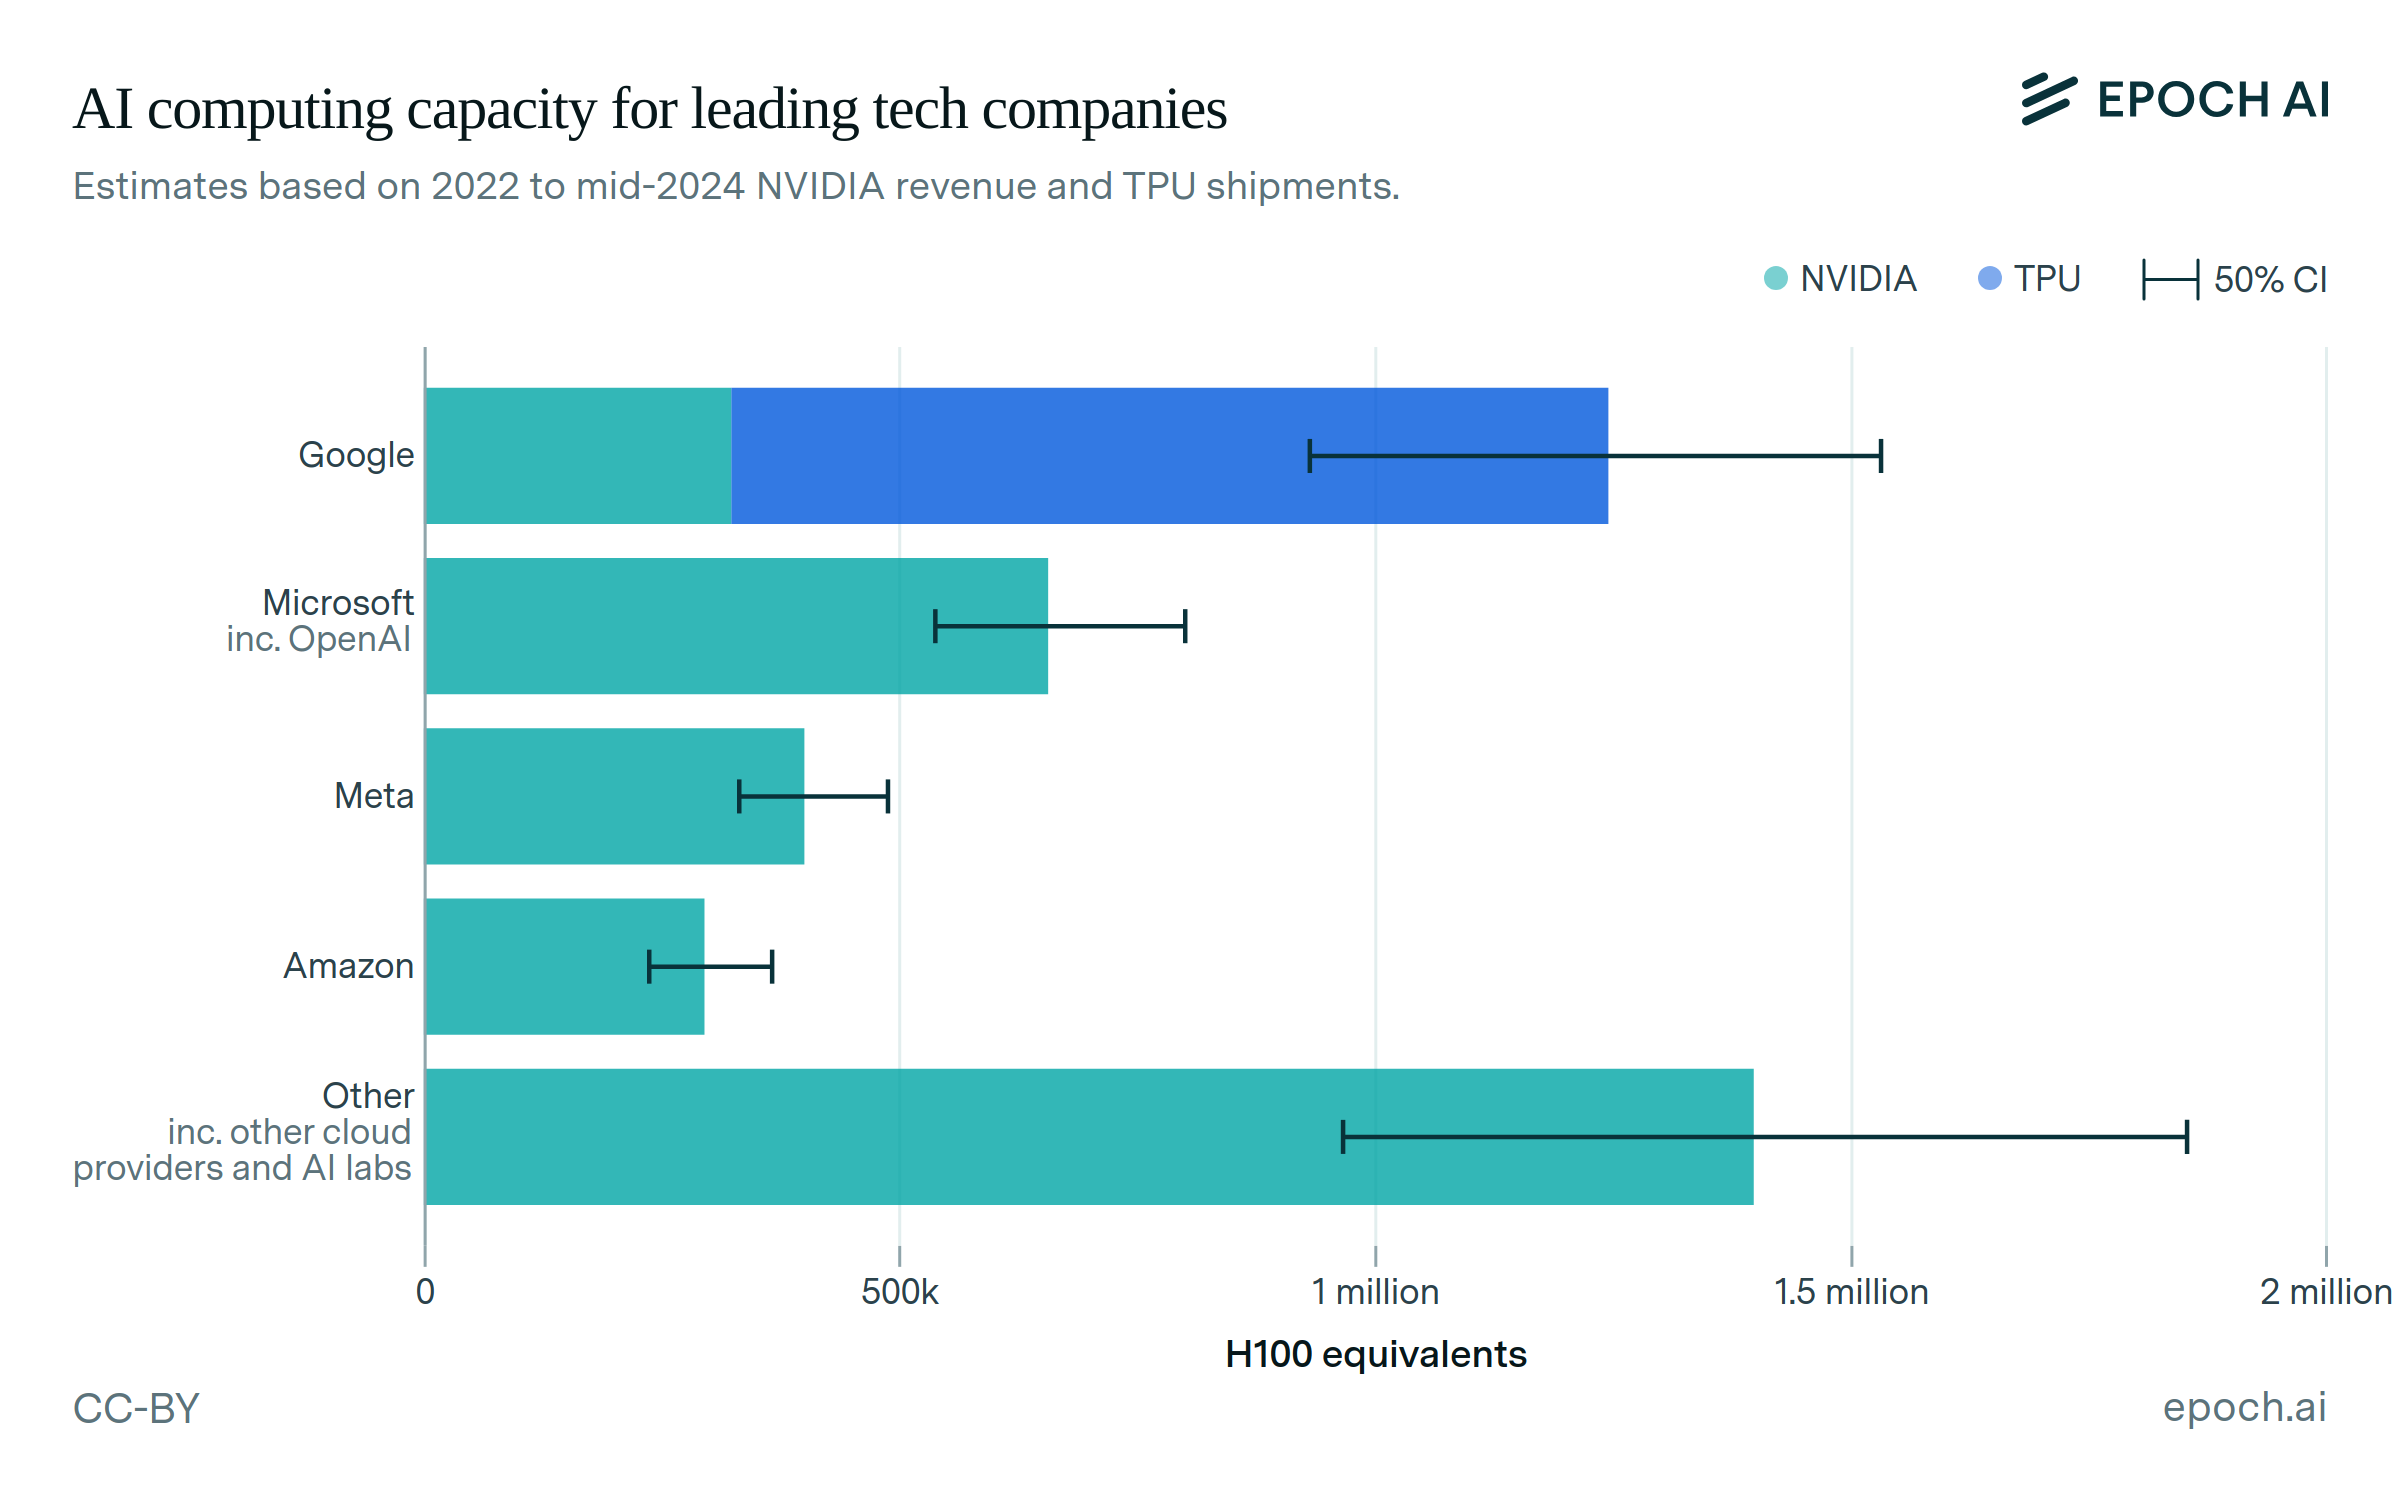
\includegraphics[height=0.5\textwidth]{images/computing-capacity}
            \caption{Estimated AI computing capacity of tech companies in mid-2024. Four companies are estimated to have purchased about half of NVIDIA's data center GPUs.~\parencite{epoch_ai_machine_learning_hardware_2024}}
        \end{figure}
    \end{frame}
    \begin{frame}
        \frametitle{Major Tech Companies Have Developed In-House AI Accelerators}
        Latest in-house chips for AI training:
        \begin{itemize}
            \item Amazon: AWS Trainium3~\parencite{tweaktown_amazon_2024}
            \item Google: Trillium~\parencite{google_tpu_2024}
            \begin{itemize}
                \item Sixth generation of TPU series that began in 2015
                \item Fully covers internal use for AI training and inference
                \item Allows them to train AI models for roughly a third of the compute cost compared to labs using NVIDIA hardware.~\parencite{epoch_notable_ai_models_2025}
            \end{itemize}
            \item Microsoft: Azure Maia 100~\parencite{microsoft_azure_maia_2023}
            \begin{itemize}
                \item First chip designed by Microsoft
            \end{itemize}
            \item Meta: MTIA v2~\parencite{meta_mtia_2024}
        \end{itemize}
    \end{frame}
    \begin{frame}
        \begin{figure}
            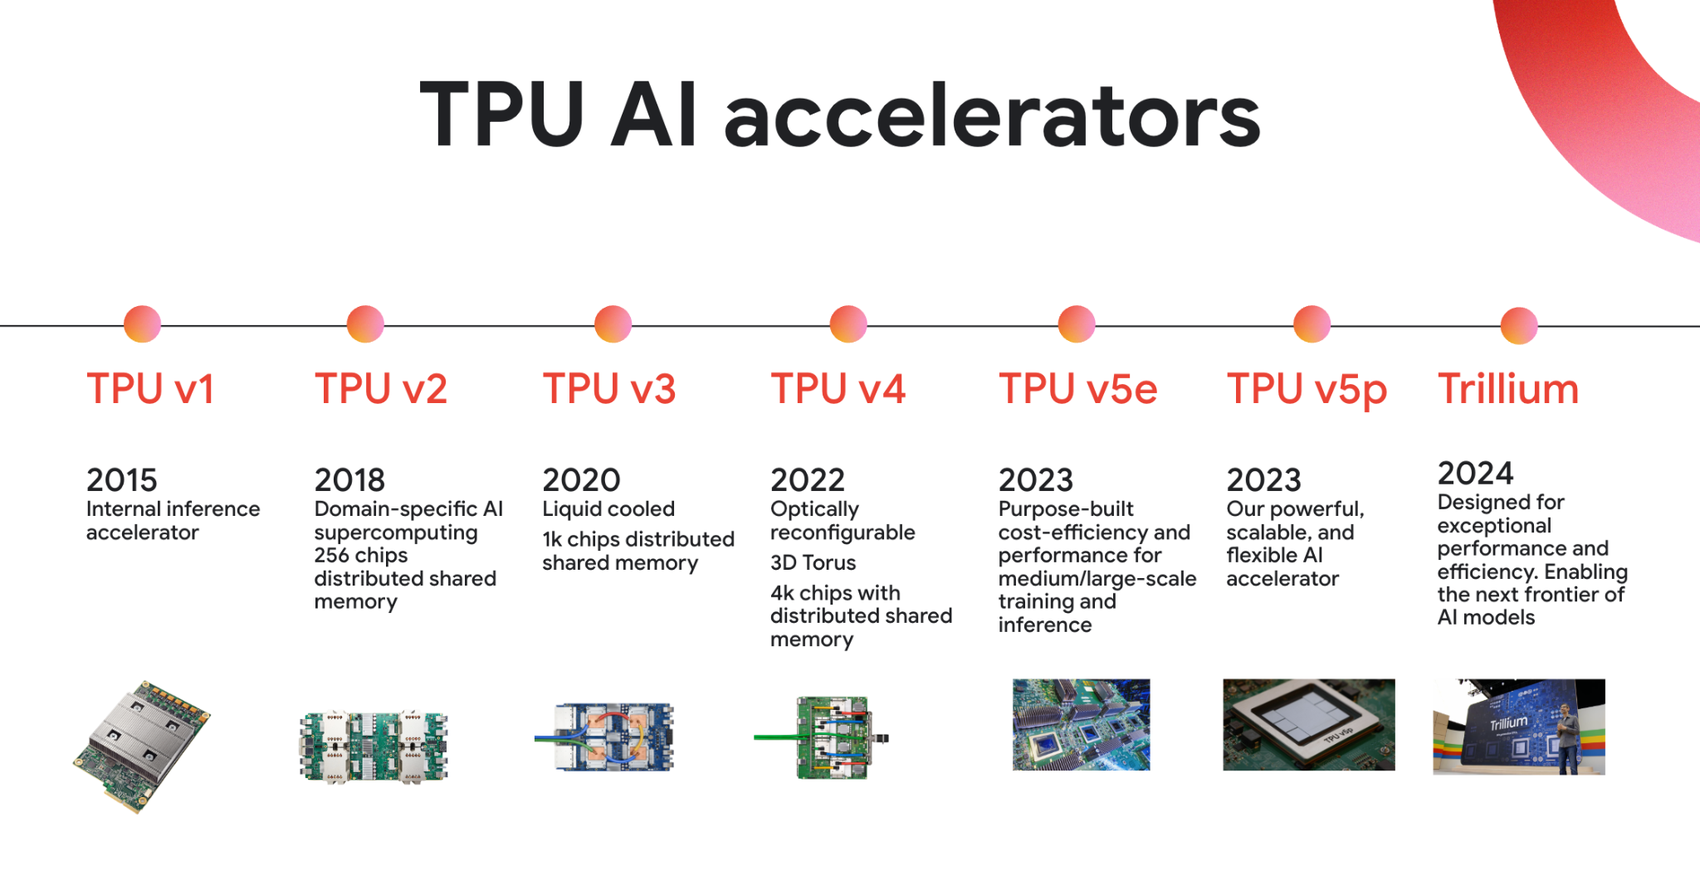
\includegraphics[height=0.5\textwidth]{images/tpu-history}
            \caption{Timeline of Google's TPU AI accelerators from TPU v1 in 2015 to Trillium, the sixth generation, in 2024~\parencite{google_tpu_2024}}
        \end{figure}
    \end{frame}
    \begin{frame}
        \frametitle{Current Situation of AI Accelerator Supply Chain}
        \begin{itemize}
            \item The production of AI accelerators is constrained by advanced chip packaging and high-bandwidth memory (HBM) availability.
            \begin{itemize}
                \item TSMC’s CoWoS process—critical for integrating logic and HBM—is expanding, but new packaging facilities require significant capital investment and highly specialized equipment.
                \item HBM supply remains tight, with current volumes nearly fully committed until 2026.
            \end{itemize}
            \item Projections indicate an annual growth in GPU production between 30\% and 100\%, yet estimates vary considerably.
            \item Competition among AI labs means that individual actors may only access a limited fraction of the total chip supply.
            \begin{itemize}
                \item Projections suggest manufacturing capacity sufficient for roughly 100 million H100-equivalent GPUs, with estimates ranging from 20 to 400 million, to be dedicated to training.
                Considering all factors, this would be \alert{roughly 5 times the estimated minimum requirements}.
            \end{itemize}
        \end{itemize}
    \end{frame}
    
    \begin{frame}
        \frametitle{Chips: In a Nutshell}
        \begin{itemize}
            \item Hardware used for AI training has evolved from graphics cards to specialized AI accelerators, with future directions including ASICs, in-memory computing, and experimental technologies like photonic and neuromorphic computing.
            \item NVIDIA dominates the AI hardware market, experiencing a 10x increase in data center revenue over two years while maintaining huge profit margins.
            \item Major tech companies including Google, Amazon, Meta and Microsoft have developed their own AI accelerators to reduce reliance on NVIDIA and lower costs, with Google's TPU series showing particular maturity.
            \item The computing capacity for AI is highly concentrated, with these four companies estimated to have purchased about half of all NVIDIA data center GPUs.
            \item While manufacturing constraints exist, particularly in chip packaging and high-bandwidth memory, current projections (with high uncertainty) suggest the chip industry can produce enough GPUs for AI training through 2030.
        \end{itemize}
    \end{frame}


    \section{Power}
    \begin{frame}
        \frametitle{What the Hell Is a Gigawatt?}
        \begin{itemize}
            \item 2 to 4 MW: Capacity of a wind turbine
            \item 10 to 30 MW: Mid-sized data center (non-AI)
            \item 50 MW: Large factory
            \item 5 to 300 MW: Small modular reactor (SMR)
            \item 1 GW: Nuclear power plant with single mid-sized reactor
            \item 2.1 GW: Peak load of Berlin grid (3.8 million residents)~\parencite{stromnetz_berlin_faktenblatt_2024}
            \item 7.6 GW: Peak load of Switzerland (9 million residents) in 2024~\parencite{swissgrid_netzlast_2025}
        \end{itemize}
    \end{frame}
    \begin{frame}
        \frametitle{How Much Power Could a Training Run in 2030 Require?}
        \begin{itemize}
            \item Epoch estimates a 24x increase in energy efficiency by 2030
            \begin{itemize}
                \item 4x through hardware efficiency improvements
                \item 2x through switching from FP16 to FP8 for training
                \item 3x through increasing the lengths of training runs
            \end{itemize}
            \item To sustain the current trajectory, interconnected data centers with a capacity of approximately \alert{6 gigawatts} working on one training run would be required
            \item Problem: Gigawatt-scale data centers can require significant upgrades to the local power infrastructure which can take many years
            \item Solution 1: Bringing data center and power generation as close together as possible, either by using existing or building new power generation
            \item Solution 2: Training on geographically distributed data centers
            \begin{itemize}
                \item It's currently unclear how well this works due to bandwidth constraints
            \end{itemize}
        \end{itemize}
    \end{frame}
    \begin{frame}
        \frametitle{How Much Power Might AI Require in Total?}
        \begin{itemize}
            \item A report released by the U.S. Department of Energy in December 2024 finds that data centers consumed about 4.4\% of total U.S. electricity in 2023 and are expected to consume approximately 6.7 to 12\% of total U.S. electricity by 2028.~\parencite{doe_2024}
            \item The PJM Interconnection, the largest regional transmission organization (RTO) in the U.S., forecasted in January 2025 that its peak load would grow 36\% in the next 10 years. As recently as 2022, they forecasted no peak load growth over the same time frame.~\parencite{pjm_2025}
            \item Federal, state and local governments, utility companies, energy companies, RTOs and technology companies are well aware of this challenge and taking action.
            \item While the U.S. is accustomed to flat electricity demand in the past few decades, a ramp-up of this size appears manageable with these actions.
        \end{itemize}
    \end{frame}
    \begin{frame}
        \begin{figure}
            \begin{columns}
                \begin{column}{0.5\textwidth}
                    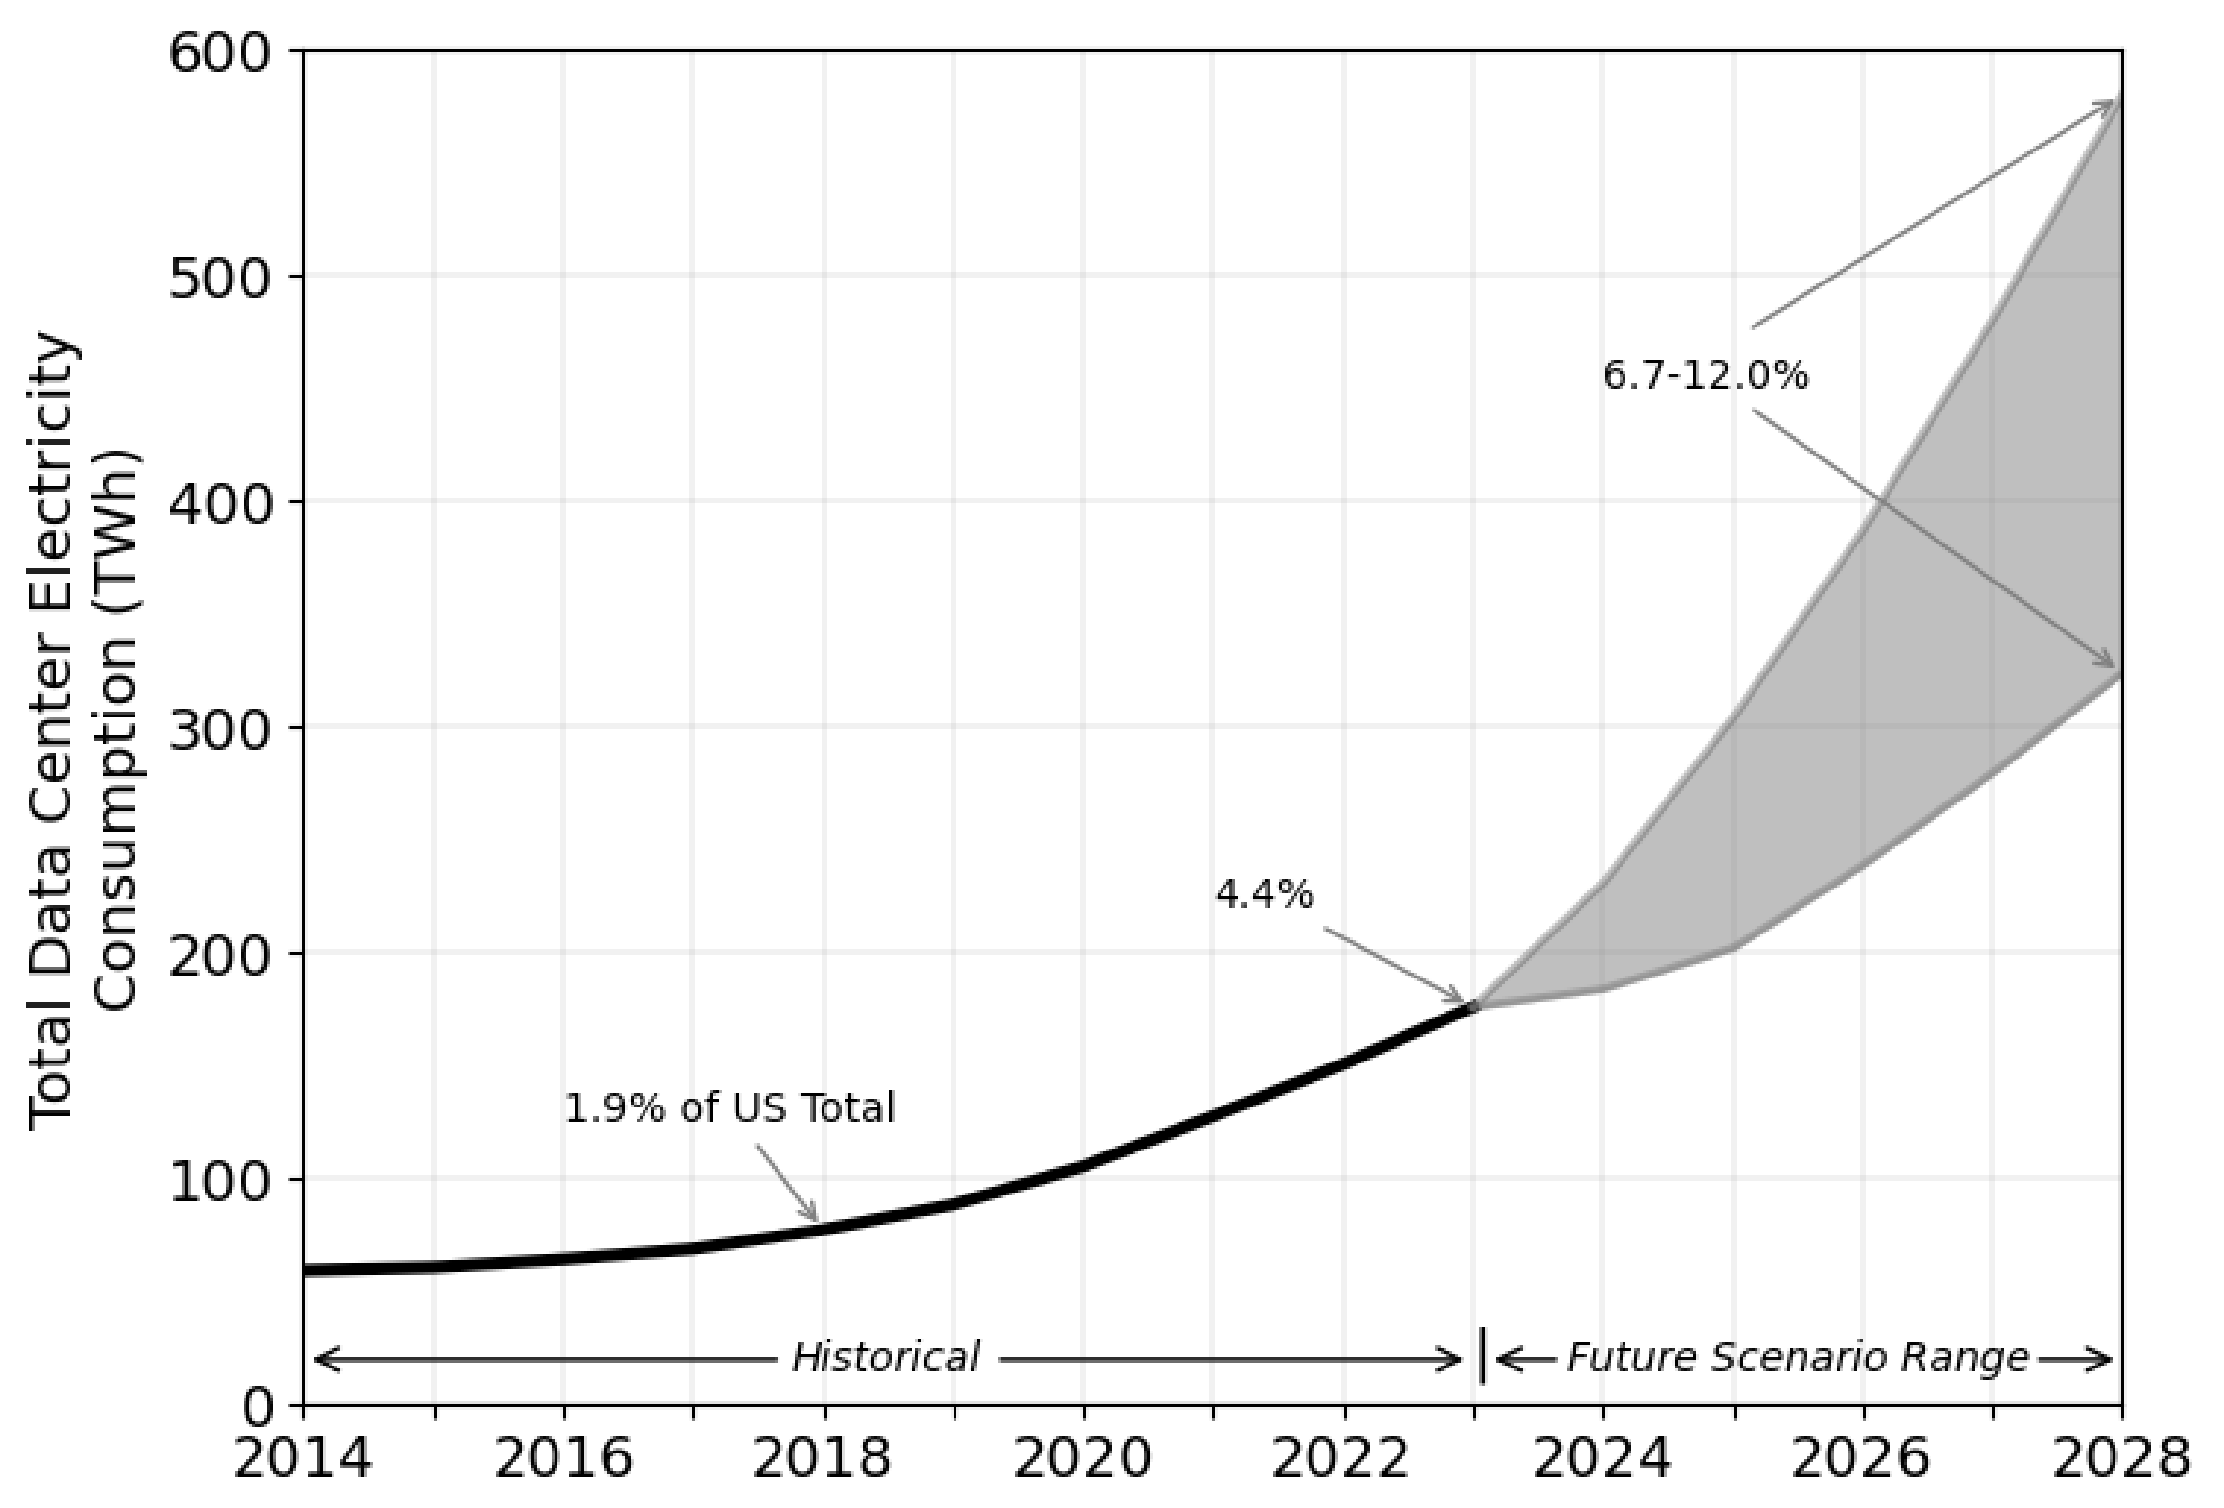
\includegraphics[width=\linewidth]{images/2024-united-states-data-center-energy-usage-report}
                \end{column}
                \begin{column}{0.5\textwidth}
                    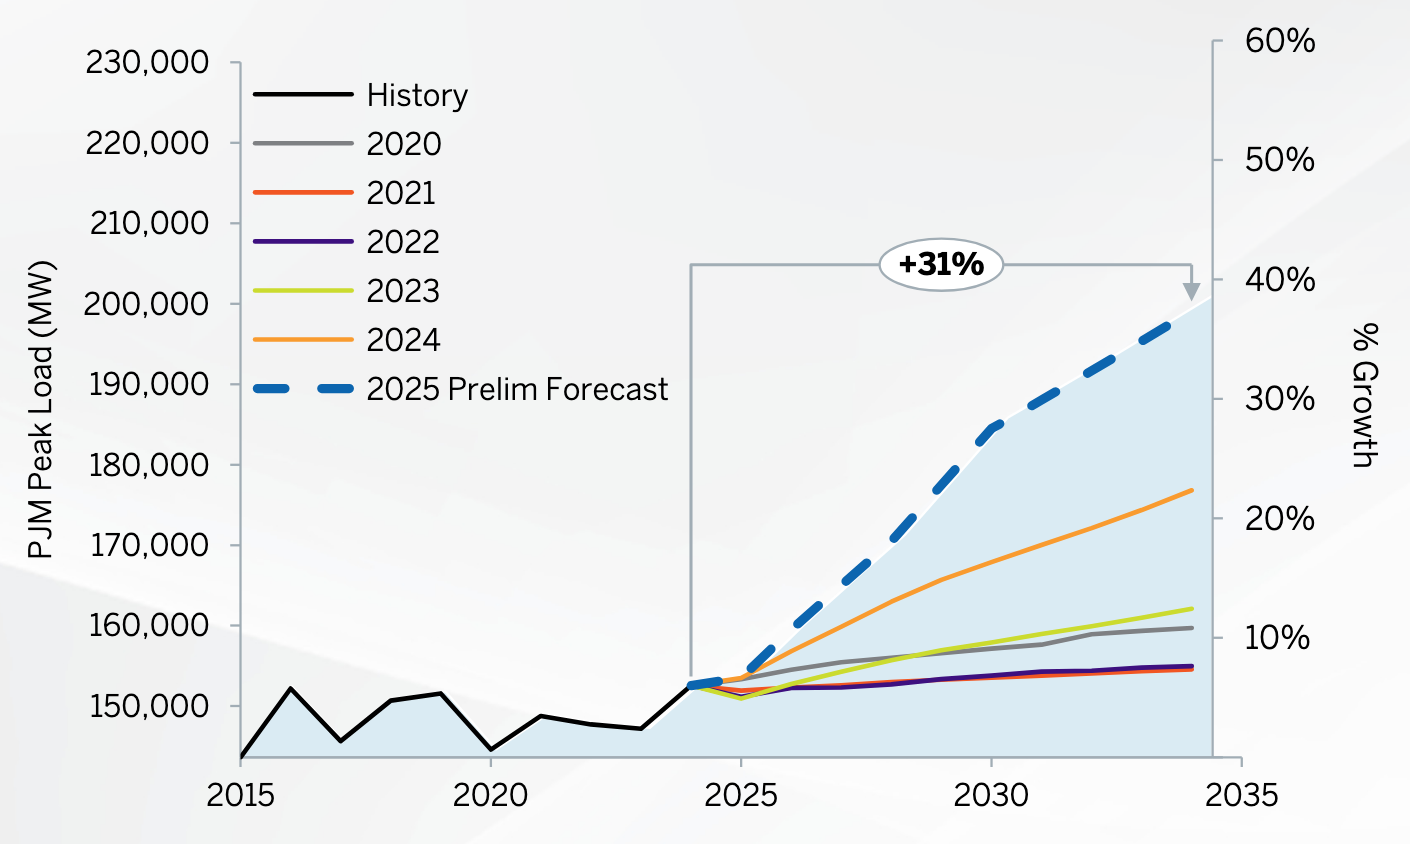
\includegraphics[width=\linewidth]{images/pjm-peak-load-growth-forecast}
                \end{column}
            \end{columns}
            \caption{Expected total U.S. data center electricity use from 2023 to 2028 (left) and forecasted peak load growth in the PJM Interconnection from 2024 to 2034 (right).}
        \end{figure}
    \end{frame}
%    \begin{frame}
%        \frametitle{Tech Companies Sign Huge Power-Purchasing Agreements}
%        \begin{itemize}
%            \item Amazon
%            \begin{itemize}
%                \item
%            \end{itemize}
%            \item Google
%            \begin{itemize}
%                \item
%            \end{itemize}
%            \item Microsoft
%            \begin{itemize}
%                \item Signed largest ever corporate agreement to purchase renewable energy in May 2024, with 10.5 GW to be built by 2030 for an estimated \$11.5+ billion.~\parencite{the_verge_microsoft_2024}
%                \item Signed agreement in September 2024 to restart the Three Mile Island nuclear power plant and purchase all its output for the next 20 years.~\parencite{constellation_energy_constellation_2024}
%            \end{itemize}
%            \item Meta
%            \begin{itemize}
%                \item
%            \end{itemize}
%        \end{itemize}
%    \end{frame}
    \begin{frame}
        \frametitle{How Big Are The Biggest Data Centers Currently?}
        \begin{itemize}
            \item For context: GPT-4 was trained on around 25,000 NVIDIA A100 (roughly 20 MW) in 2022~\parencite{epoch_notable_ai_models_2025}
            \item Scaling beyond this presents novel challenges, including large-scale construction, networking, hardware failures, bandwidth constraints, cooling and power
            \item Leading tech companies recently finished data centers with around 100,000 NVIDIA H100 (roughly 150 MW), offering roughly 12x compute~\parencite{patel_transcript_2025}
            \item Meta is training their Llama 4 models on a cluster with more than 100,000 NVIDIA H100s~\parencite{wired_metas_2024}
            \item No models trained on these were released in 2024 due to the time needed for experimentation, training, post-training and safety evaluations, but are being released during 2025 (GPT-5, Claude 4, Llama 4, Grok 3).
        \end{itemize}
    \end{frame}
    \begin{frame}
        \frametitle{How Big Are the Data Centers Planned for 2025?}
        \begin{itemize}
            \item Microsoft is said to be building 5 interconnected data centers for AI training with 100,000 NVIDIA Blackwell GPUs each for a total of 500,000 GPUs using 1 GW while other tech giants have similar plans.~\parencite{patel_10b_2024}
        \end{itemize}
    \end{frame}
    \begin{frame}
        \frametitle{Building New Nuclear Reactors for Data Centers?}
        \begin{itemize}
            \item Amazon
            \begin{itemize}
                \item Looked for a ``Principal Nuclear Engineer'' to ``build internal and external nuclear product and fuel strategy roadmaps [\ldots] for AWS data centers''~\parencite{amazon_principal_2024}
                \item Signed three agreements to support ``nuclear energy projects—including enabling the construction of several new Small Modular Reactors (SMRs)''~\parencite{amazon_nuclear_deals_2024}
            \end{itemize}
            \item Google
            \begin{itemize}
                \item Signed an agreement to ``purchase nuclear energy from multiple small modular reactors (SMR) to be developed by Kairos Power''~\parencite{google_kairos_2024}
            \end{itemize}
            \item Microsoft
            \begin{itemize}
                \item Looked for a ``Principal Program Manager Nuclear Technology'' to explore SMRs to power data centers~\parencite{microsoft_principal_2023} and hired directors for ``Nuclear Technologies'' and ``Nuclear Development Acceleration''~\parencite{data_center_dynamics_microsoft_2024}
            \end{itemize}
            \item Meta
            \begin{itemize}
                \item Request for proposals to ``identify nuclear energy developers [\ldots] targeting 1-4 gigawatts (GW) of new nuclear generation capacity in the U.S.''~\parencite{meta_accelerating_2024}
            \end{itemize}
        \end{itemize}
    \end{frame}
    \begin{frame}
        \frametitle{Gigawatt-Scale Data Centers Next to Nuclear Power Plants?}
        \begin{itemize}
            \item Constellation Energy and Vistra are in discussions with large tech companies to power data centers with up to several gigawatts of capacity co-located with existing nuclear power plants through behind-the-meter agreements.~\parencite{data_center_frontier_gigawatt_2024, wall_street_journal_tech_2024, bloomberg_constellation_2024}
            \item Under such an agreement, a data center would be build next to an existing nuclear power plant and directly connected with it, requiring a significant portion or even all of the output of the plant.
        \end{itemize}
    \end{frame}
    \begin{frame}
        \frametitle{What Are the Biggest Data Center Currently Planned for the Future?}
        \begin{itemize}
            \item The biggest known plans for data centers are from Amazon, Microsoft, OpenAI (through Stargate) and Meta, each having roughly 1 to 2 gigawatts of capacity.
            \item These projects will either use existing large substations and power plants or build new dedicated power plants or use a combination of these two approaches.
            \item The hardware costs of a 2 GW project alone (when using NVIDIA hardware) will be on the order of \$50 billion.
            \item Each of these projects will rank among the most expensive factories ever built and among the most expensive megaprojects in U.S. history.
        \end{itemize}
    \end{frame}
    \begin{frame}
        \frametitle{X.AI Builds Gigawatt-Scale Data Center in Memphis, Tennessee}
        \begin{itemize}
            \item X.AI is building a gigawatt-scale data center inside a closed Electrolux factory in Memphis, Tennessee
            \item Located next to a 1.1 GW natural gas plant and a tapped-off natural gas line.
            \item Improvised using mobile gas generators, battery packs and chillers parked outside the building.
            \item Currently being built out to 200,000 NVIDIA Hopper GPUs (roughly 300 MW).
            \item Build-out to 1 million NVIDIA Blackwell GPUs (roughly 2 GW) and construction of a natural gas plant planned.
        \end{itemize}
    \end{frame}
    \begin{frame}
        \frametitle{Amazon's Nuclear-Powered Data Center Plan}
        \begin{itemize}
            \item In March 2024, AWS acquired the Cumulus campus intended to have 960 MW capacity once finished, right besides the 2.5 GW Susquehanna nuclear power plant in Pennsylvania.
            \item The site was initially intended for crypto mining companies and will be expanded in 120 MW increments into a gigawatt-scale campus.
            \item The project faces pushback from utility companies and consumers and regulatory challenges, including the FERC blocking the proposed expansion in a first decision.
            \begin{itemize}
                \item Talen Energy is challenging the decision.~\parencite{data_center_dynamics_susquehanna_2025}
            \end{itemize}
        \end{itemize}
    \end{frame}
    \begin{frame}
        \begin{figure}
            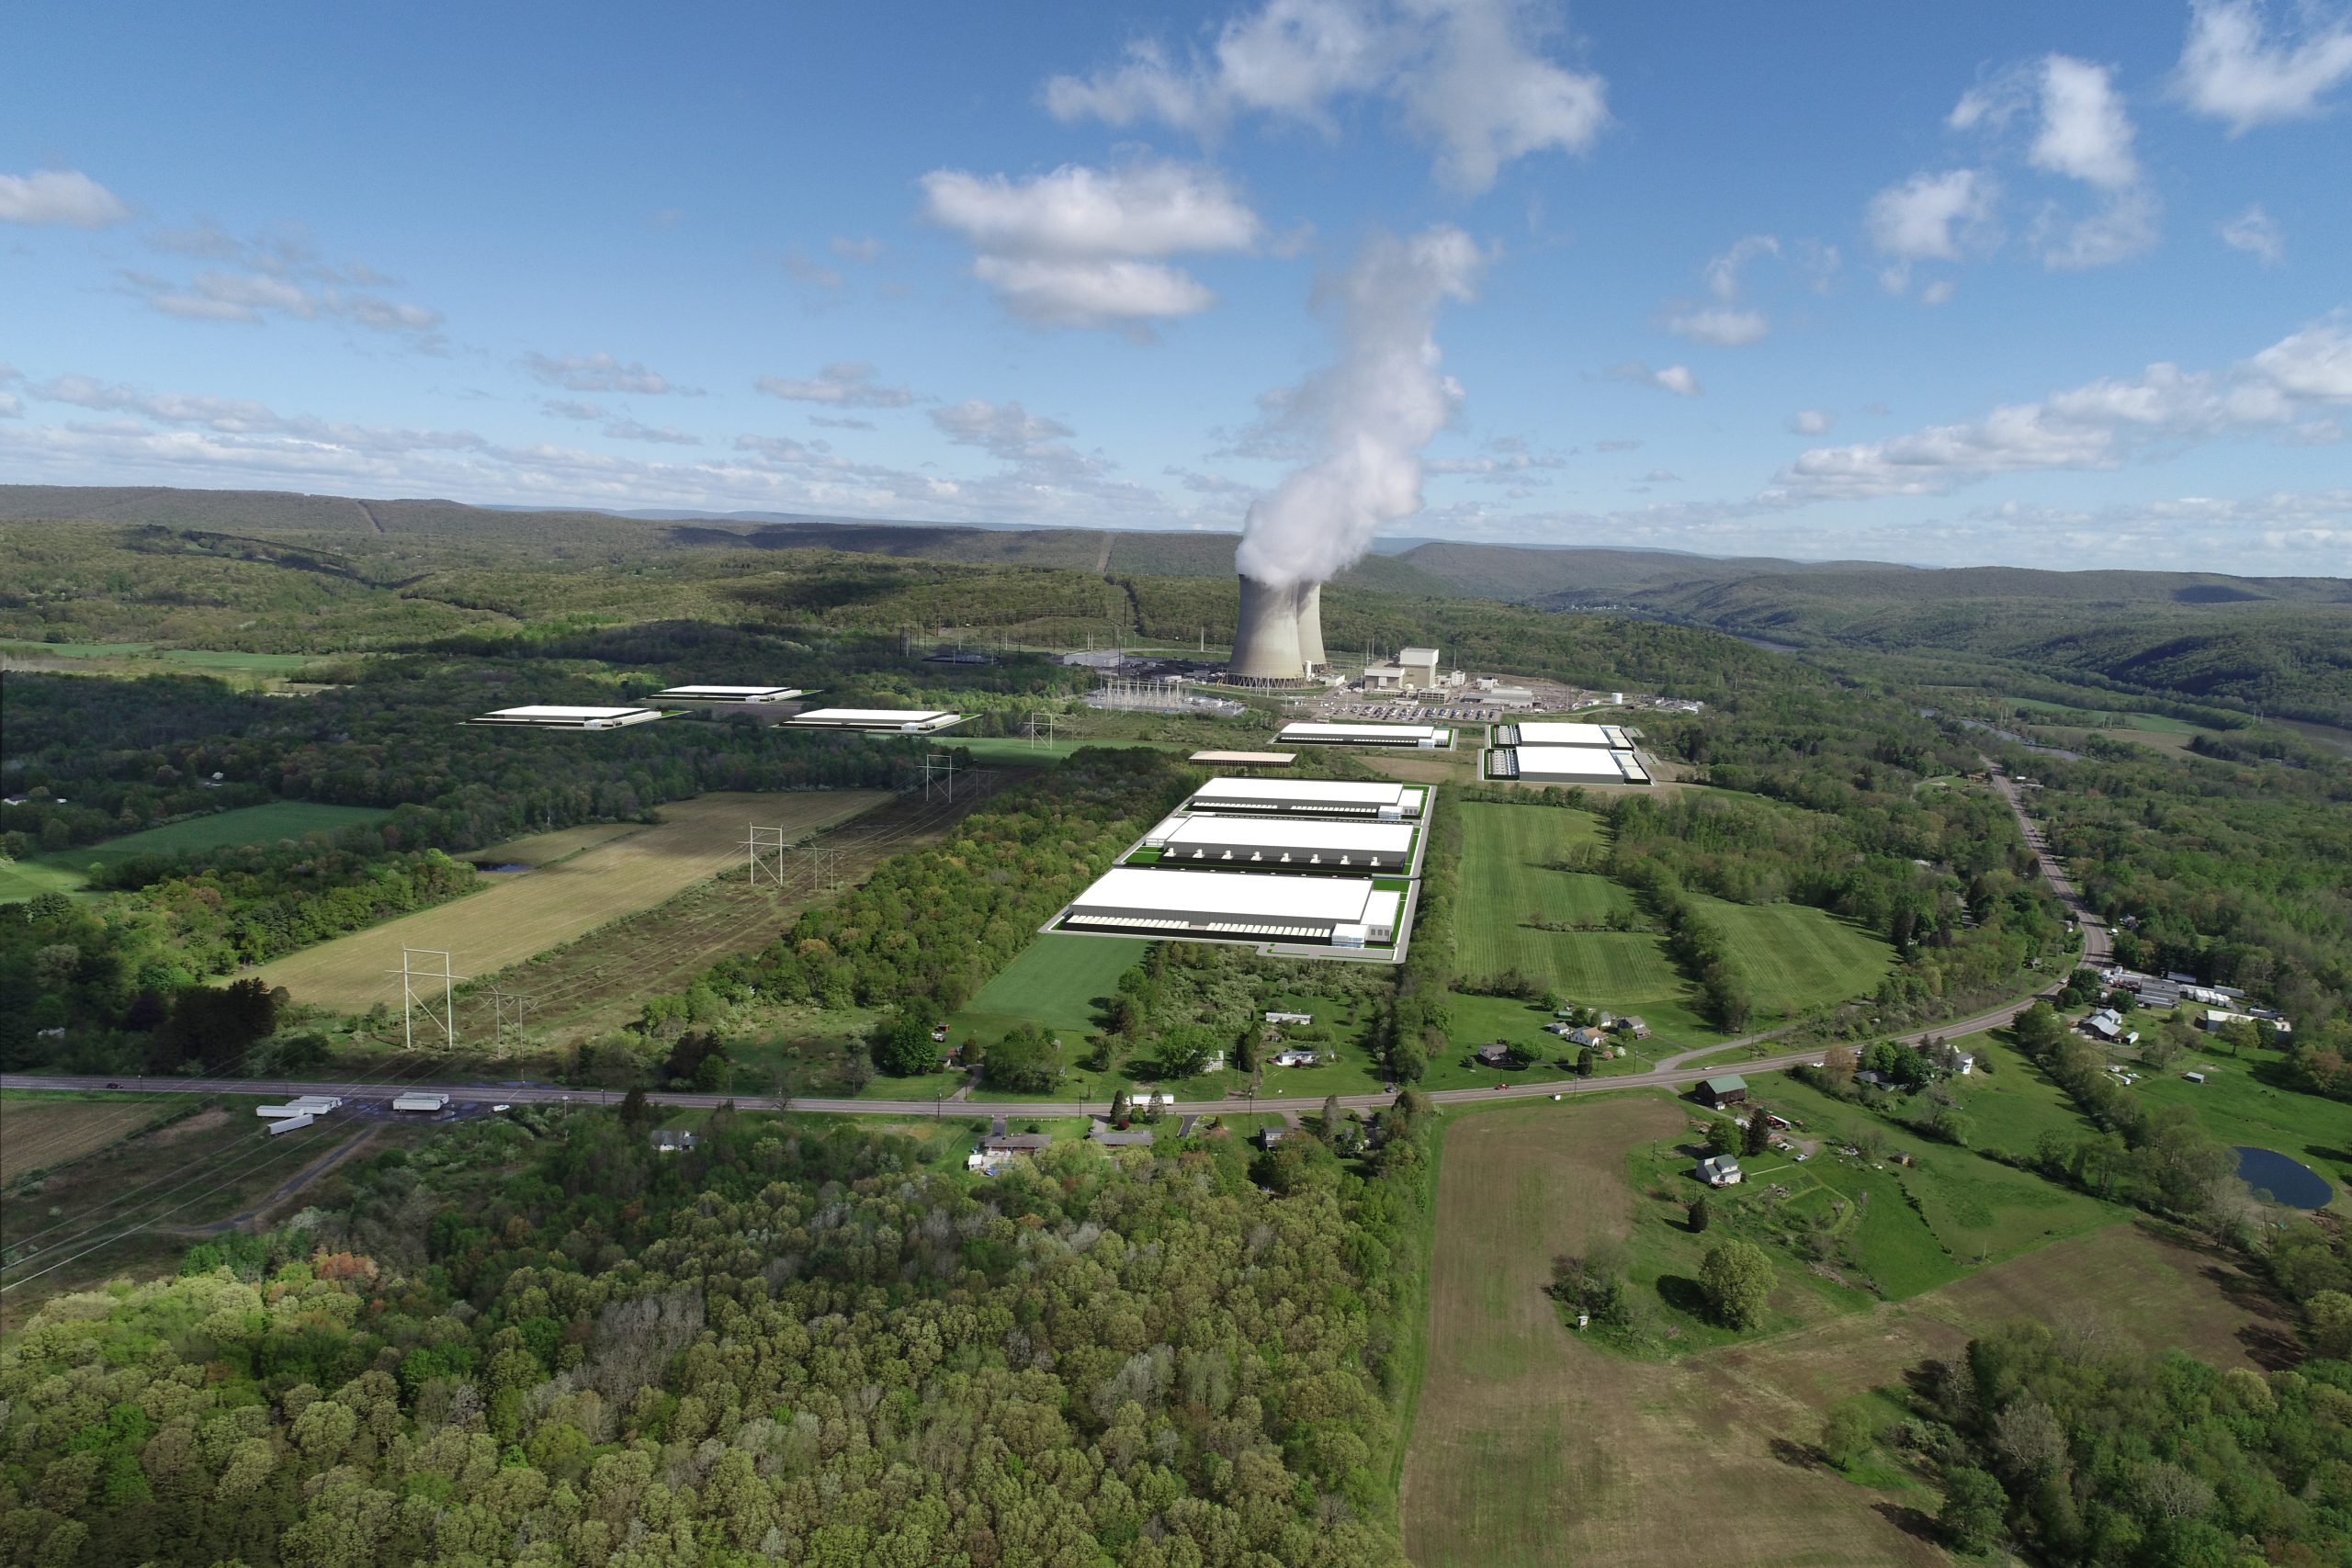
\includegraphics[height=0.5\textwidth]{images/cumulus-campus-rendering}
            \caption{Rendering from Talen Energy of how the Cumulus data center campus next to the Susquehanna nuclear power plant could look like in the future. Amazon's plans might differ.}
        \end{figure}
    \end{frame}
    \begin{frame}
        \frametitle{Microsoft's Gigawatt-Scale Data Center in Wisconsin}
        \begin{itemize}
            \item Microsoft is constructing data centers in Mount Pleasant, Wisconsin that are expected to have a total capacity of 1.5 gigawatts by mid-2027.~\parencite{patel_stanford_lecture_2024}
            \item Announced in May 2024 by Microsoft President Brad Smith and U.S. President Joe Biden.~\parencite{microsoft_wisconsin_2024}
        \end{itemize}
    \end{frame}
    \begin{frame}
        \begin{figure}
            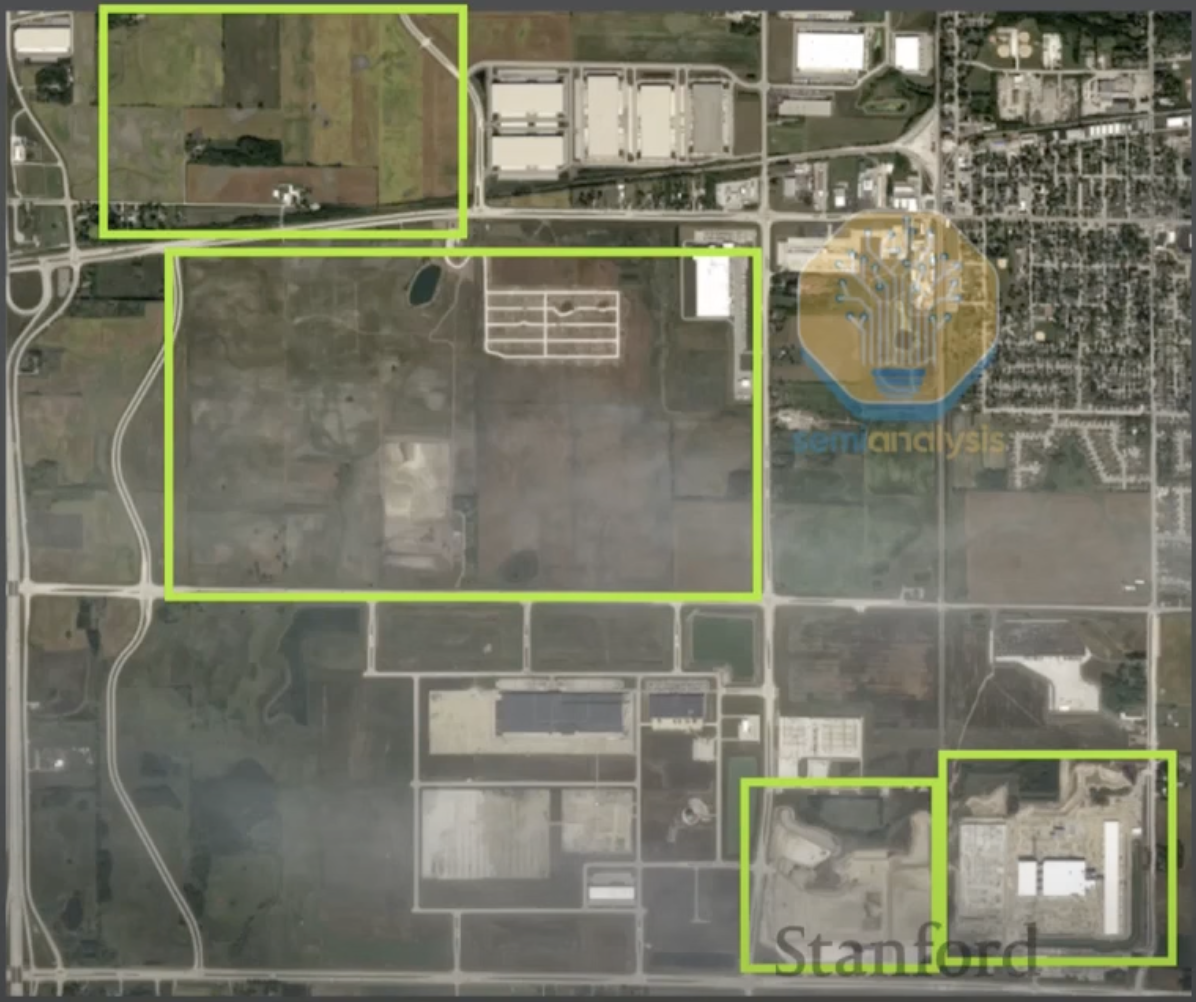
\includegraphics[height=0.5\textwidth]{images/microsoft-mount-pleasant-satellite-footage}
            \caption{Satellite footage of Microsoft's data center sites in Mount Pleasant, Wisconsin with construction sites and expansion plans highlighted.~\parencite{patel_stanford_lecture_2024}}
        \end{figure}
    \end{frame}
    \begin{frame}
        \frametitle{OpenAI's Project Stargate}
        \begin{itemize}
            \item Initially leaked in March 2024 as a \$100 billion supercomputer project planned by OpenAI and Microsoft featuring millions of chips and requiring up to 5 gigawatts of power~\parencite{the_information_stargate_2024}
            \item Officially announced at the beginning of U.S. President Trump's first press conference back in office~\parencite{white_house_youtube_trump_infrastructure_remarks_2025}
            \begin{itemize}
                \item Joint venture created by OpenAI, SoftBank, Oracle and MGX
                \item No funding from the U.S. government or Microsoft
                \item Plans to invest up to \$500 billion in AI infrastructure for OpenAI, but so far only \$100 billion have been committed and the rest is questionable
            \end{itemize}
            \item First data center is under construction in Abilene, Texas and is reportedly 2.2 GW with estimated hardware costs of roughly \$50 billion~\parencite{patel_transcript_2025}
            \begin{itemize}
                \item Located at a site for a large data center project planned since 2021 and close to two natural gas pipelines.
                \item Two substations built and eight data hall buildings under construction currently.
            \end{itemize}
        \end{itemize}
    \end{frame}
    \begin{frame}
        \begin{figure}
            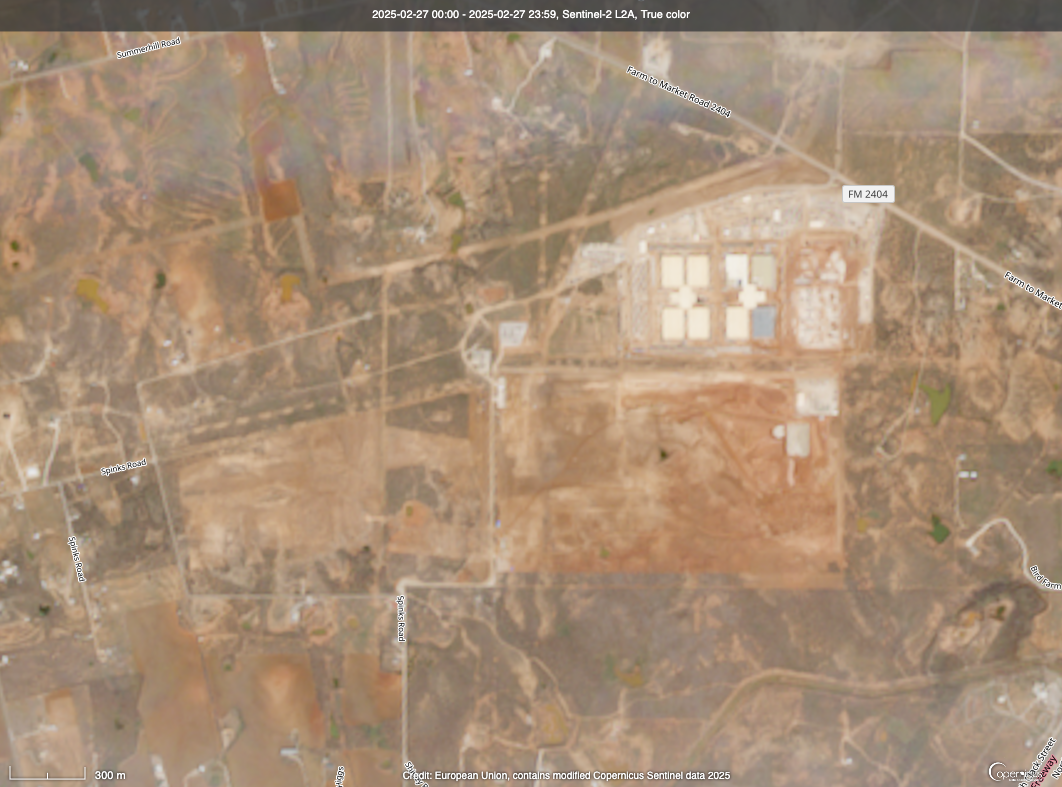
\includegraphics[height=0.5\textwidth]{images/stargate-1-copernicus-feb-2025}
            \caption{Satellite footage from February 27, 2025 of the construction of Stargate Site 1 in Abilene, Texas. Clearing of additional 2 km\textsuperscript{2} of land began in January 2025.~\parencite{copernicus_browser_2025}}
        \end{figure}
    \end{frame}
    \begin{frame}
        \frametitle{Meta's Plans for Gigawatt-Scale Data Centers}
        \begin{itemize}
            \item Scrapped Plan for Data Center at Nuclear Power Plant~\parencite{murphy_criddle_2024}
            \begin{itemize}
                \item Multiple complications including the discovery of a rare bee species at the location
            \end{itemize}
            \item 2+ GW Data Center in Richland Parish, Louisiana~\parencite{zuckerberg_louisiana_datacenter_2024}
            \begin{itemize}
                \item Three natural gas turbines with a combined capacity of 2.26 GW, six substations, nearly 100 miles of 500kV transmission lines, eight new 230kV transmission lines and 1.5 GW of solar and storage resources will be built.~\parencite{entergy_2025}
                \item Announced by Louisiana Governor Landry in December 2024, who said it ``is expected to be the largest private capital investment announcement in the state’s history''~\parencite{governor_of_louisiana_2024}
            \end{itemize}
            \item Possibly a 1+ GW Data Center in West Feliciana, Louisiana~\parencite{boone_2025}
            \begin{itemize}
                \item Hut 8 is building an AI data center for an undisclosed tenant
                \item 300 MW capacity in first phases and possibly up to and beyond 1 GW in future phases with possible construction of a power plant
            \end{itemize}
        \end{itemize}
    \end{frame}
    \begin{frame}
        \begin{figure}
            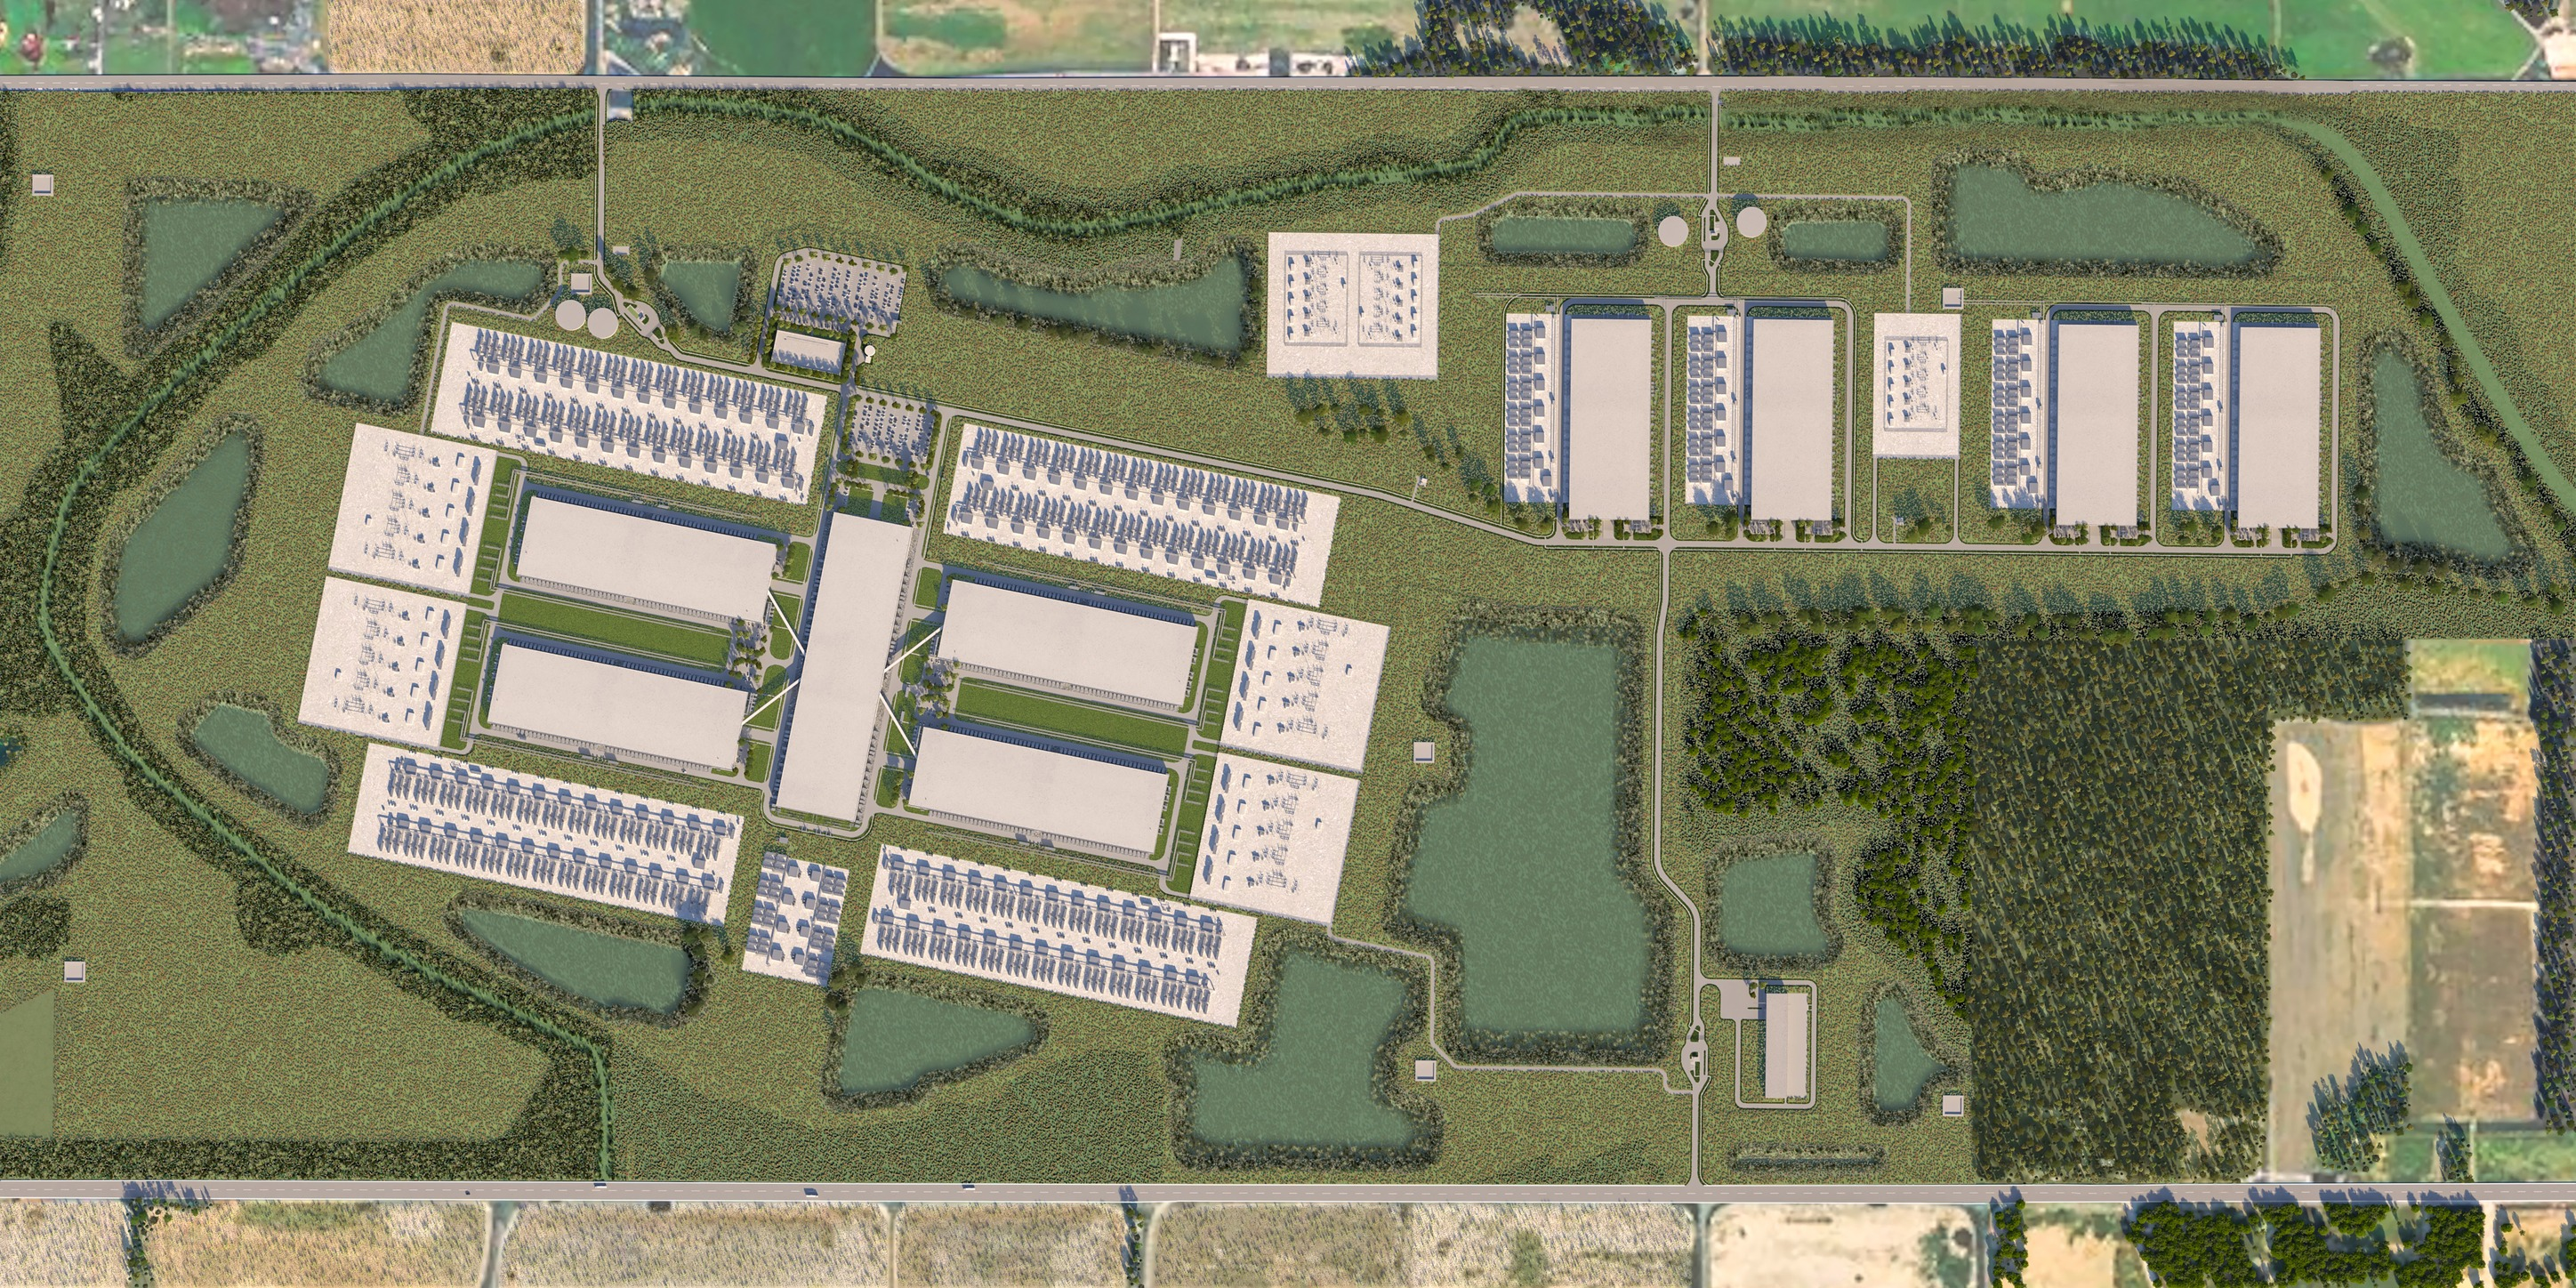
\includegraphics[height=0.5\textwidth]{images/meta_richland_parish_louisiana_data_center}
            \caption{Rendering of Meta's planned data center in Richland Parish, Louisiana, featuring a 1 km\textsuperscript{2} main complex, additional buildings and cooling ponds on a 6 km\textsuperscript{2} site~\parencite{meta_louisiana_datacenter_facebook_2024}}
        \end{figure}
    \end{frame}
    \begin{frame}
        \begin{figure}
            \begin{columns}[c]
                \begin{column}{0.5\textwidth}
                    \vspace{7pt}
                    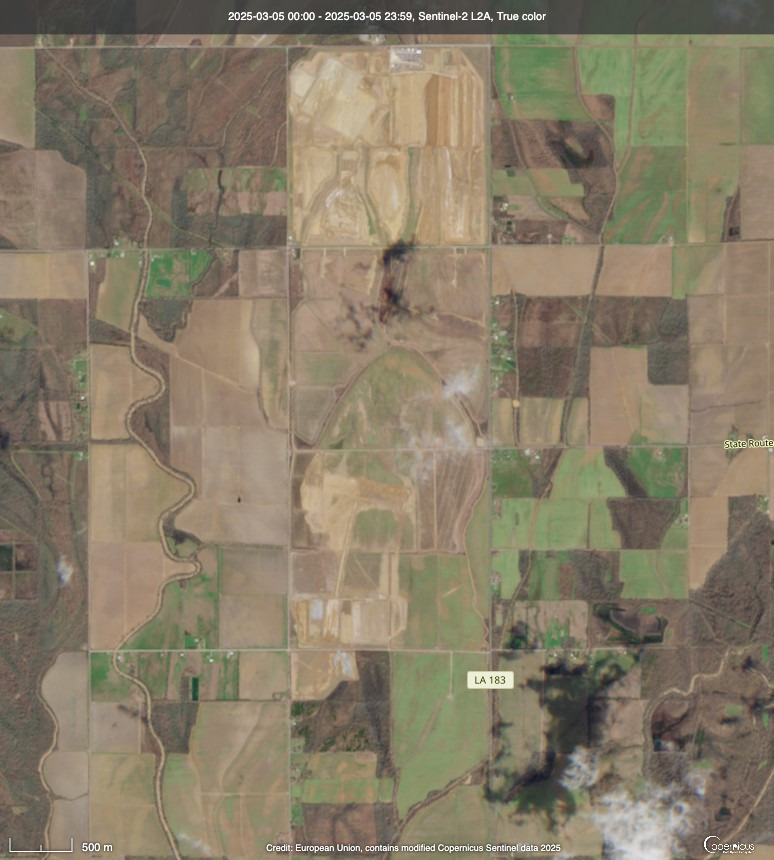
\includegraphics[height=1.2\textwidth]{images/meta_richland_parish_louisiana_satellite_footage}
                \end{column}
                \begin{column}{0.45\textwidth}
                    \caption{Satellite footage from March 5, 2025 of the construction of Meta's data center in Richland Parish, Louisiana. Clearing of 2.5 km\textsuperscript{2} of land for the construction of two natural gas plants began in November 2024, visible in the top center. Clearing for the main complex and cooling ponds began in February 2025, visible in the center.~\parencite{copernicus_browser_2025}}
                \end{column}
            \end{columns}
        \end{figure}
    \end{frame}
    \begin{frame}
        \frametitle{Power: In a Nutshell}
        \begin{itemize}
            \item Frontier AI models in 2030 could require interconnected data centers with a capacity of approximately 6 gigawatts for a single training run, posing unprecedented power infrastructure challenges.
            \item The U.S. Department of Energy and the PJM Interconnection project a significant, yet likely manageable, increase in total electricity demand, a major shift from previously flat electricity demand forecasts.
            \item Major tech companies are pursuing gigawatt-scale data centers connected to existing power plants, building new power plants, and exploring nuclear energy options through agreements with energy companies.
            \item The largest planned data centers by will each rank among the most expensive factories ever built and among the most expensive megaprojects in U.S. history.
        \end{itemize}
    \end{frame}


    \section{Geopolitics}
    \begin{frame}
        \frametitle{U.S. Leads AI Investment; U.S. and China Lead AI Research}
        \begin{itemize}
            \item 61\% of AI patents granted in 2022 were from China, while 21\% were from the U.S. and 2\% were from the EU/UK.
            \item 73\% of foundation models released in 2023 were from the U.S., while 13\% were from China and 10\% were from the EU/UK.
            \item 39\% of GitHub stars on AI projects until 2023 were on projects from the U.S., while 17\% were from the EU/UK, 8\% from China and 7\% from India.
            \item 70\% of global private investment in AI in 2023 occurred in the U.S., while 11\% occurred in the EU/UK and 8\% in China.
            \begin{itemize}
                \item In generative AI, 89\% occurred in the U.S., 3\% in the EU/UK and 3\% in China.
            \end{itemize}
            \item 897 AI companies were funded in the U.S. in 2023, while 368 were funded in the EU/UK and 122 were funded in China.
            \item All data from the 2024 AI Index Report~\parencite{stanford_university_2024}
        \end{itemize}
    \end{frame}
    \begin{frame}
        \begin{figure}
            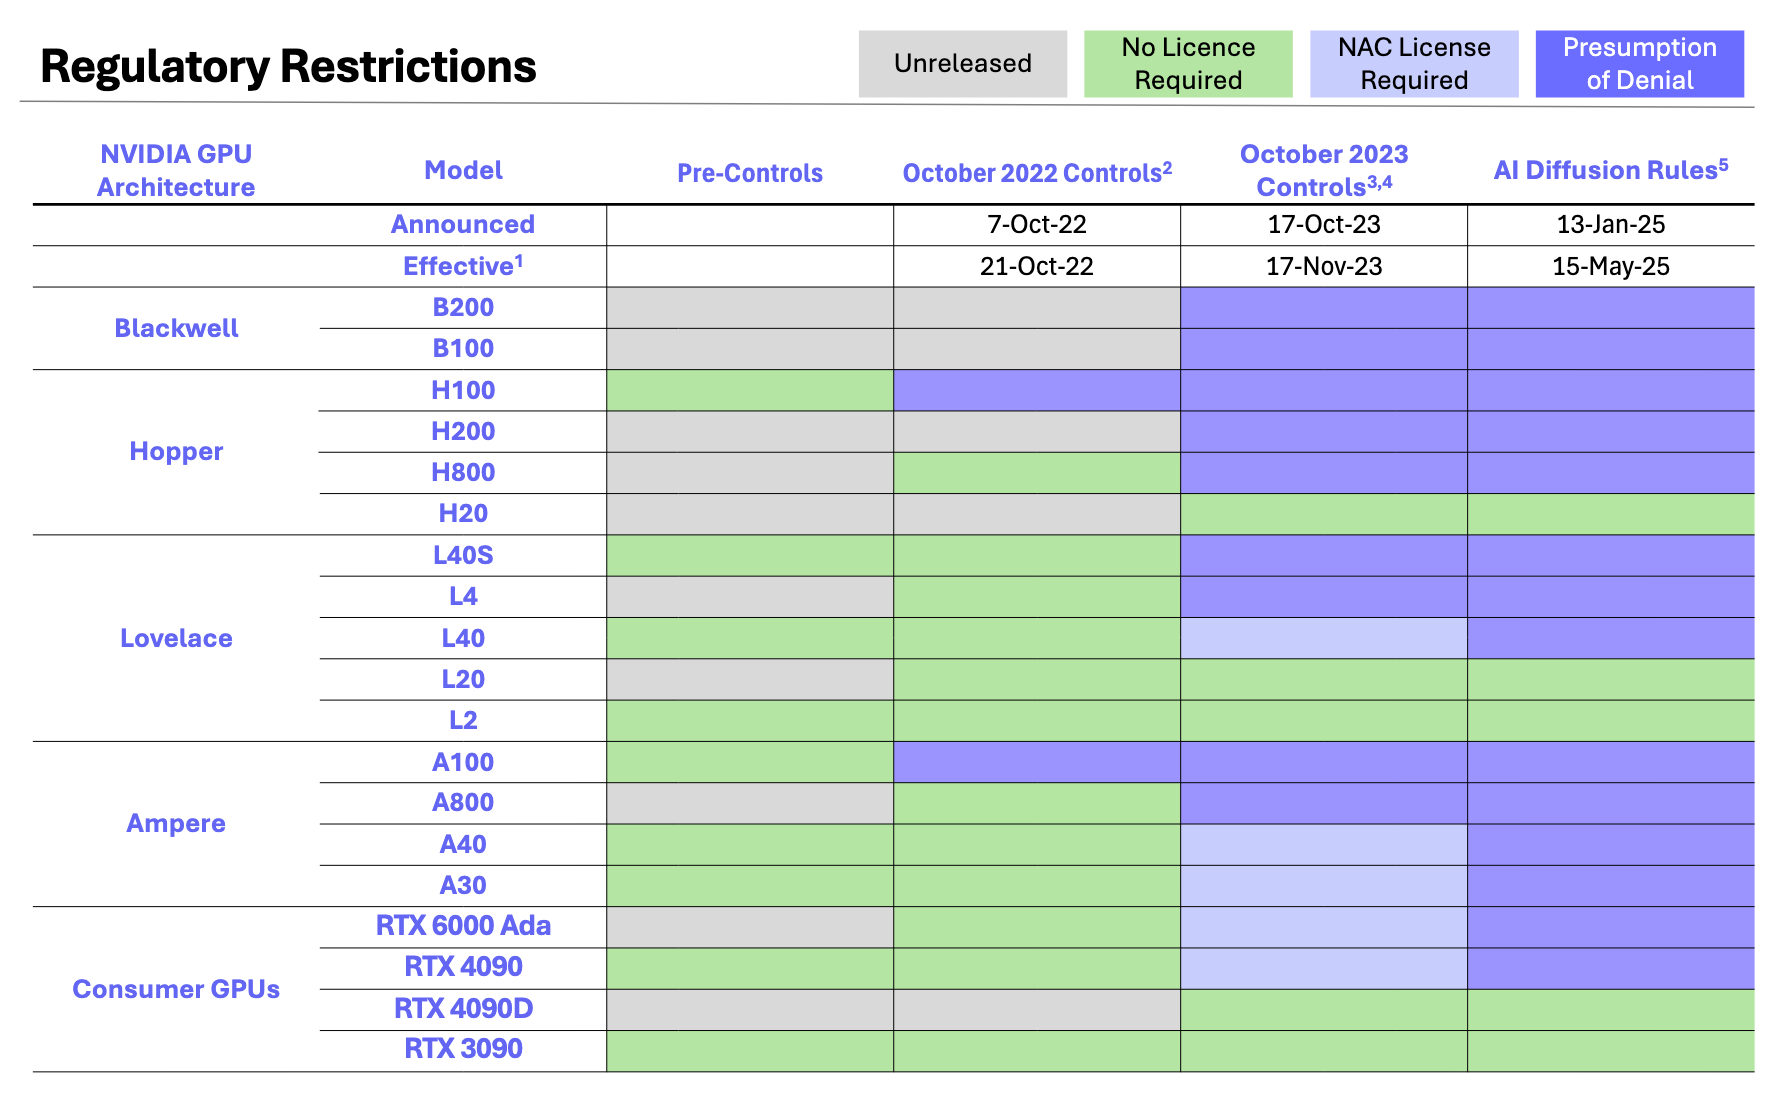
\includegraphics[height=0.48\textwidth]{images/us-chip-export-restrictions-china}
            \caption{U.S. chip export restrictions to China and affected NVIDIA GPUs. Export of the H100 was banned in October 2022, leading NVIDIA to develop the H800. Export of the H800 was banned in October 2023, leading NVIDIA to develop the H20.~\parencite{artificial_analysis_state_2025}}
        \end{figure}
    \end{frame}
    \begin{frame}
        \frametitle{Key Actions and Statements of the Biden Administration on AI}
        \begin{itemize}
            \item AI National Security Memorandum in October 2024~\parencite{white_house_memorandum_2024}
            \begin{itemize}
                \item Declares the U.S. ``must lead the world’s development of safe, secure, and trustworthy AI'', instructing federal agencies to ``streamline permitting, approvals, and incentives for the construction of AI-enabling infrastructure'' including ``clean energy generation, power transmission lines, and high-capacity fiber data links''
            \end{itemize}
            \item Order on AI Export Restrictions on January 13, 2025~\parencite{white_house_fact_sheet_2025}
            \begin{itemize}
                \item Each country except ``18 key allies and partners'' is subjected to a new import compute cap equivalent to around 20,000 NVIDIA Blackwell GPUs until 2027.
                \item Small purchases don't count against that total and companies can, under strict requirements, apply for increased caps.
            \end{itemize}
            \item Order on Advancing AI Infrastructure on January 14, 2025~\parencite{white_house_statement_2025}
            \begin{itemize}
                \item ``Lease federal sites [\ldots] to host gigawatt-scale AI data centers.''
            \end{itemize}
            \item Farewell Address on January 15, 2025
            \begin{itemize}
                \item ``Meanwhile, artificial intelligence is the most consequential technology of our time — perhaps of all time.''~\parencite{white_house_farewell_address_2025}
            \end{itemize}
        \end{itemize}
    \end{frame}
    \begin{frame}
        \frametitle{Key Actions and Statements of the Trump Administration on AI}
        \begin{itemize}
            \item Senate Hearing of Interior Secretary Burgum~\parencite{doug_burgum_senate_hearing_2025}
            \begin{itemize}
                \item ``So we're competing against someone who's going to create more electricity, produce more AI, and this could be how we lose the Cold War with [China]''
            \end{itemize}
            \item National Energy Emergency Declaration on Day 1~\parencite{white_house_national_energy_emergency_2025}
            \begin{itemize}
                \item Declared the first ever national energy emergency for several reasons including ``high demand for energy and natural resources to power the next generation of technology''
            \end{itemize}
            \item Announcement of ``Project Stargate'' on Day 2~\parencite{white_house_youtube_trump_infrastructure_remarks_2025}
            \begin{itemize}
                \item ``I'm going to help a lot through emergency declarations because we have an emergency.
                We have to get this stuff built.
                So they have to produce a lot of electricity, and we'll make it possible for them to get that production done very easily at their own plants''
            \end{itemize}
            \item Speech of Vice President Vance at the AI Action Summit in Paris~\parencite{ucsb_remarks_2025}
            \begin{itemize}
                \item ``Now, at this moment, we face the extraordinary prospect of a new industrial revolution, one on par with the invention of the steam engine or Bessemer steel.''
            \end{itemize}
        \end{itemize}
    \end{frame}
    \begin{frame}
        \frametitle{Europe, and Particularly France, Step Up On AI}
        \begin{itemize}
            \item In February 2025, the EU launched InvestAI, a public-private partnership ``to mobilise €200 billion for investment in AI, including a new European fund of €20 billion for AI gigafactories'' including ``four future AI gigafactories across the EU'' with ``around 100 000 last-generation AI chips''.~\parencite{european_commission_2025}
            \item French President Macron announced in February 2025 that France has secured €109 billion in ``private French and foreign investments'' in AI ``for the coming years''.~\parencite{le_monde_intelligence_2025}
            \item A few days earlier after a meeting with UAE President bin Zayed, he announced €30-50 billion investments from French and Emirati investors into a 1 GW AI data center in France.~\parencite{data_center_dynamics_france_2025}
            \item Mistral AI, the leading AI startup in Europe, has raised almost €1 billion so far and is headquartered in Paris.
        \end{itemize}
    \end{frame}
    \begin{frame}
        \frametitle{Geopolitics: In a Nutshell}
        \begin{itemize}
            \item The U.S. leads the world in AI investment, while both the U.S. and China lead in AI research.
            \item The U.S. has implemented increasingly stringent chip export restrictions to China (and now almost all countries of the world), limiting access to AI accelerators.
            \item Both the Biden and Trump administrations have elevated AI to a matter of national security and economic competitiveness, with both taking measures to streamline construction of gigawatt-scale data centers and Trump declaring the first ever national energy emergency partly to power AI.
            \item Europe, led by France, is mounting a significant response with multi-billion euro investments to build data centers, though still lagging behind the U.S.
        \end{itemize}
    \end{frame}
    
    \begin{frame}[allowframebreaks]{References}
        \printbibliography
    \end{frame}
\end{document}
